Discutiamo ora la teoria BCS, che è la teoria microscopica della superconduttività. Le tre ipotesi principali di questa teoria sono:
\begin{enumerate}[leftmargin=0.6cm]
   \item Esiste un'interazione attrattiva tra elettroni, il che è inatteso se si considera solo l'interazione coulombiana. È quindi necessario introdurre un meccanismo microscopico che, come vedremo, è mediato dalle vibrazioni del reticolo cristallino e che induce un'interazione attrattiva efficace tra elettroni.
   \item Quando è presente anche una debolissima interazione attrattiva tra elettroni, gli elettroni vicini al livello di Fermi risultano instabili, nel senso che uno stato in cui due elettroni formano una cosiddetta coppia di Cooper, cioè una particolare combinazione di due elettroni con opportune relazioni tra momento e spin, ha un'energia più bassa rispetto allo stato di elettroni liberi. Questo è il cosiddetto problema di Cooper e conduce all'identificazione della funzione d'onda dello stato fondamentale del superconduttore.
   \item Una caratteristica fondamentale della funzione d'onda dello stato fondamentale del superconduttore è che essa rappresenta uno stato a molti corpi in cui tutti gli elettroni in prossimità del livello di Fermi formano coppie di Cooper. Questo stato è detto stato coerente a molti corpi.
\end{enumerate}
\section{Interazione elettrone--fonone}
\subsection{DFT e interazione efficace}

Partiamo dall'interazione attrattiva. Sappiamo che gli elettroni interagiscono tramite l'interazione coulombiana
\begin{equation*}
   V(\vb{r} - \vb{r'})
   =\frac{e^2}{4 \pi \varepsilon_0 |\vb{r} - \vb{r'}|}
\end{equation*}
che è repulsiva e rappresenta l'interazione tra elettroni ``nudi'', cioè elettroni nel vuoto. Nei metalli la situazione è diversa perché, quando gli elettroni si muovono nel materiale, tutti gli altri elettroni devono in un certo senso ``lasciarli passare''. Questo si traduce in un'interazione efficace tra elettroni dovuta al fatto che, oltre alla repulsione coulombiana elettronica, entra in gioco anche il principio di esclusione di Pauli, che contribuisce al tipo di interazione tra elettroni.\\
Questo porta al concetto di quasi-particelle, introdotto da Landau, che descrive il fatto che quando un elettrone si muove in un mare elettronico, come in un metallo, si produce una sorta di ridistribuzione degli altri elettroni attorno ad esso. Questo fenomeno è descritto, nel linguaggio della teoria del funzionale della densità (DFT), tramite la cosiddetta \emph{exchange-correlation hole}. Si tratta di un modo tecnico per descrivere il fatto che l'interazione efficace tra elettroni deriva dalla combinazione della repulsione coulombiana e del principio di esclusione di Pauli.\\
Nella DFT si introduce una funzione di correlazione a coppie $g$ del gas elettronico, che dipende dalla distanza tra due elettroni, cioè $g=g(|\vb{r} - \vb{r'}|)$. Essa misura la probabilità relativa di trovare un elettrone in $\vb{r'}$ dato che un altro si trova in $\vb{r}$. Questa funzione è tale che, quando i due elettroni hanno lo stesso spin (entrambi up o entrambi down), per distanze molto piccole questo fattore si annulla.\mn{La funzione $g(\vb{r},\vb{r}')$ modifica effettivamente la repulsione coulombiana, tenendo conto del fatto che gli elettroni non possono stare nello stesso punto (principio di esclusione di Pauli, effetto di scambio) e tendono a evitare zone di alta densità (effetto di correlazione coulombiana).} Questo riflette il fatto che due elettroni con lo stesso spin non possono occupare la stessa posizione. Viceversa, per distanze grandi, $g$ tende a $1$.
\begin{figure}[H]
   \centering
   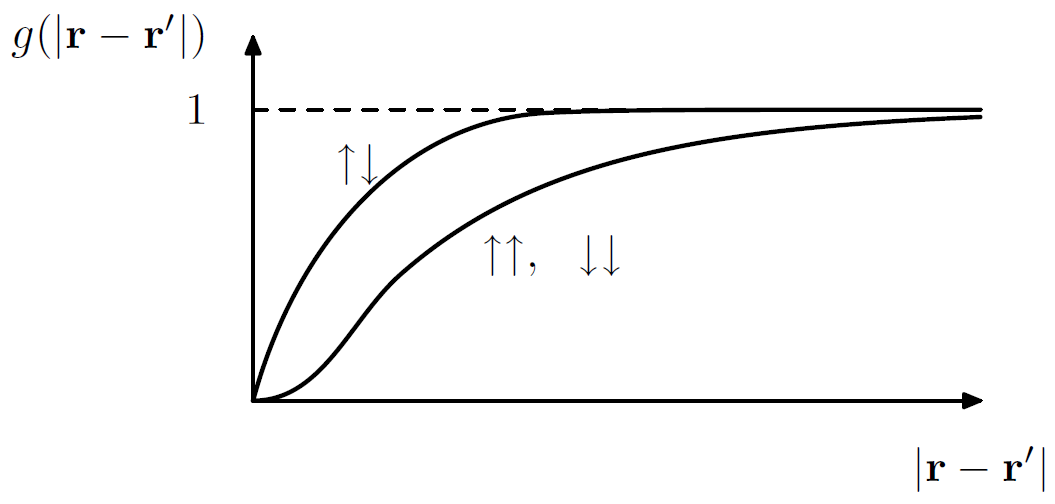
\includegraphics[width=0.7\textwidth]{immagini/funzione_di_correlazione.png}
\end{figure}
\hspace{-0.6cm}Questo effetto è detto \emph{exchange hole}, nel senso che descrive l'effetto dell'interazione di scambio che impedisce agli elettroni di occupare la stessa posizione. A questo si aggiunge la repulsione coulombiana, che introduce un costo energetico quando gli elettroni sono vicini: questo costituisce la parte di correlazione del problema exchange-correlation.\\
Il punto importante è comprendere il meccanismo complessivo, che deriva dall'azione combinata della repulsione coulombiana e del principio di esclusione. Il modo più semplice per descrivere questo effetto di schermaggio è utilizzare un potenziale coulombiano schermato, in cui lo screening è descritto dal modello di Thomas--Fermi come un decadimento esponenziale:
\begin{equation*}
   V_{\rm TF}
   = \frac{e^2}{4 \pi \varepsilon_0} \frac{1}{|\vb{r} - \vb{r'}|} e^{-|\vb{r} - \vb{r'}|/r_{\rm TF}}
\end{equation*}
Questo introduce di fatto una lunghezza caratteristica molto più corta per la repulsione coulombiana, che in linea di principio agirebbe a tutte le distanze.\\
\subsection{Interazione con i fononi}
Finora abbiamo considerato solo la parte elettronica, ma per comprendere la cosa accade nella transizione superconduttiva è necessario includere anche l'effetto delle vibrazioni del reticolo. L'indizio sperimentale che l'effetto da includere fosse proprio questo è l'effetto isotopico, cioè la dipendenza della temperatura critica dalla massa isotopica. Questo infatti suggerisce che il fenomeno coinvolge il moto dei nuclei attorno alle loro posizioni di equilibrio, cioè le vibrazioni del reticolo, ossia i fononi.\\
Il meccanismo può essere descritto tramite diagrammi di Feynman, che rappresentano un modo semplice per descrivere a livello grafico ciò che accade.
\begin{figure}[H]
   \centering
   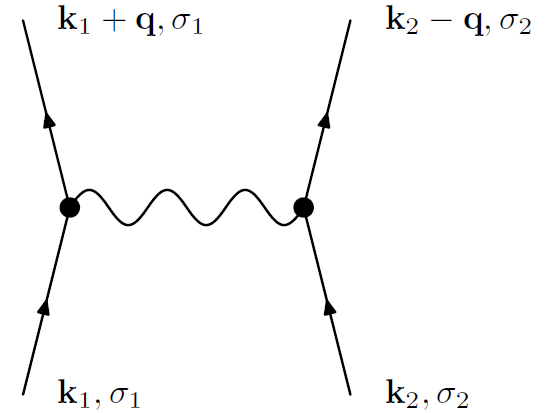
\includegraphics[width=0.45\textwidth]{immagini/diagramma_di_Feynman_1.png}
\end{figure}
\hspace{-0.6cm}Consideriamo un elettrone in uno stato di Bloch, caratterizzato quindi da due numeri quantici: $n$, legato alla sua energia, e $\vb{k}_2$, che è il suo momento. Inoltre esso possiede spin $\sigma_2$. In questa descrizione diagrammatica esso è rappresentato da una freccia.\\
Questo elettrone può emettere un fonone con quantità di moto $\hbar\vb{q}$, modificando quindi a causa di questa interazione, descritta da un punto nel diagramma, il proprio momento in $\vb{k}_2 - \vb{q}$. Il suo spin rimarrà invece invariato.\\
I fononi sono rappresentati da linee ondulate nel diagramma, per indicare la loro diversa natura e statistica. Il momento che acquisisce il fonone è $\hbar\vb{q}$, in modo che il momento totale sia conservato.\\
Un secondo elettrone, caratterizzato da $(\vb{k}_1,\sigma_1)$, può interagire con lo stesso fonone, acquisendo un momento maggiore $\vb{k}_1 + \vb{q}$, come se avesse assorbito il fonone, mantenendo lo stesso spin.\\
Questo processo rappresenta un'interazione efficace tra due elettroni, $(\vb{k}_1,\sigma_1)$ e $(\vb{k}_2,\sigma_2)$, mediata dallo scambio di un fonone.\mn{Questo meccanismo è generale: particelle fermioniche possono interagire tramite lo scambio di bosoni, come avviene anche nella fisica delle particelle.}\\
Ribadiamo il fatto che questa è una descrizione pittorica: non stiamo ancora spiegando perché un elettrone interagisca con un fonone. Per capire l'origine dell'interazione bisogna considerare il reticolo cristallino.\\
Consideriamo un cristallo con un atomo per cella unitaria. Possiamo studiare quali vibrazioni sono possibili nel reticolo. In particolare sappiamo che in questo caso possiamo avere un modo longitudinale e due modi trasversali.\\
Se vogliamo scrivere l'energia del reticolo includendo le vibrazioni, dobbiamo considerare che ogni vibrazione ha una certa frequenza $\omega$ e quindi un'energia $\hbar\omega$. Questa energia dipende dal momento, il quale è differente a seconda del tipo di modo.\\
Possiamo descrivere questi modi come oscillatori armonici e quindi la loro energia può essere scritta nella forma quantistica che conosciamo per l'oscillatore armonico. Se $a^{\dag}_{\vb{q},\lambda}$ e $a^{\vphantom{\dag}}_{\vb{q},\lambda}$ sono gli operatori di creazione e annichilazione di fononi con frequenza $\omega_{\vb{q},\lambda}$, allora l'energia dei modi del cristallo con un atomo per cella unitaria può essere espressa come una somma sui modi $\omega$ e sulle polarizzazioni $\lambda$:
\begin{equation*}
   H
   = \sum_{\vb{q},\lambda} \hbar \omega^{\vphantom{\dag}}_{\vb{q},\lambda} a_{\vb{q},\lambda}^{\dag} a^{\vphantom{\dag}}_{\vb{q},\lambda}
\end{equation*}
Questi modi, se interpretati nello spazio reale (mentre sono stati introdotti nello spazio dei momenti), corrispondono a spostamenti degli atomi rispetto alle loro posizioni di equilibrio. Indichiamo tali spostamenti con $\delta \vb{R}_i$, dove $\vb{R}_i$ è la posizione dell'$i$-esimo atomo del reticolo. Essi possono essere espressi in termini delle coordinate dei modi $(\vb{q},\lambda)$; in generale si ha una somma su tutti i modi, con il fattore tipico che compare quando si descrive la coordinata di un oscillatore armonico in termini degli operatori $a$ e $a^{\dag}$:
\begin{equation*}
   \delta \vb{R}_i
   =\sum_{\vb{q},\lambda} \vb{e}_{\vb{q},\lambda} \sqrt{\frac{\hbar}{2 M \omega_{\vb{q},\lambda}}} \qty( a^{\dag}_{\vb{q},\lambda} + a_{-\vb{q},\lambda} ) e^{i \vb{q} \vdot \vb{R}_i}
\end{equation*}
Un tale spostamento del reticolo cristallino produrrà una modulazione della densità di carica degli elettroni e del potenziale efficace per gli elettroni nel solido, $V_1(\vb{r})$. Possiamo definire il potenziale di deformazione come
\begin{equation*}
   \delta V_1(\vb{r})
   =\sum_i \delta \pdv{V_1(\vb{r})}{\vb{R}_i} \delta \vb{R}_i
\end{equation*}
Vediamo ora quali sono le conseguenze di questi spostamenti per gli elettroni che si muovono nel reticolo.
\begin{figure}[H]
   \centering
   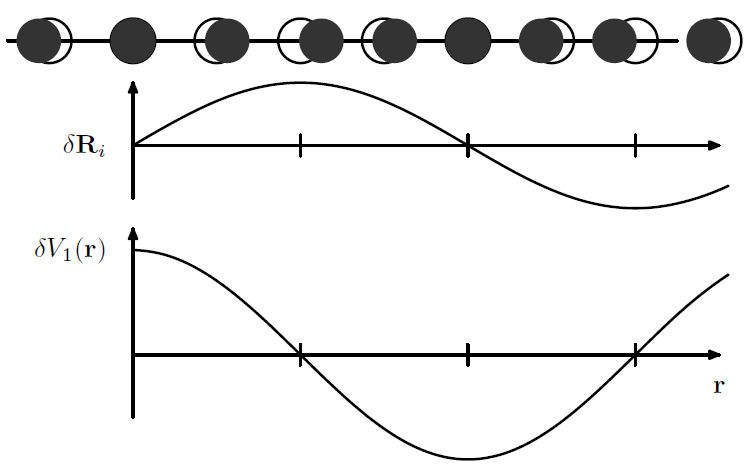
\includegraphics[width=0.7\textwidth]{immagini/reticolo_cristallino.png}
\end{figure}
\hspace{-0.6cm}La figura mostra schematicamente cosa accade quando gli atomi non si trovano più nelle loro posizioni di equilibrio, ma sono soggetti a uno spostamento $\delta \vb{R}_i$ associato a un modo di vibrazione del reticolo. Gli atomi risultano quindi leggermente dislocati: alcuni possono rimanere praticamente fermi, mentre altri si spostano in direzioni opposte in modo periodico lungo il reticolo.\\
Dal punto di vista fisico, questo è cruciale perché gli atomi in un metallo sono ioni, quindi portano carica positiva. Di conseguenza, una loro ridistribuzione nello spazio implica una modulazione della densità di carica positiva: si formano regioni in cui la densità è maggiore rispetto all'equilibrio e regioni in cui è minore.\\
Un elettrone che si muove nel reticolo “vede” quindi un potenziale elettrico che non è più uniforme: nelle regioni in cui la densità di carica positiva è maggiore, il potenziale è più attrattivo, mentre nelle regioni in cui è minore è meno attrattivo (o relativamente repulsivo rispetto alla configurazione uniforme).\\
Questo porta all'idea chiave: la vibrazione del reticolo genera una modulazione del potenziale che tende ad attirare gli elettroni verso le regioni di maggiore densità ionica. In tali regioni si crea una sorta di buca di potenziale in cui gli elettroni sono energeticamente favoriti a trovarsi.\\
Se consideriamo due elettroni liberi di muoversi nel reticolo, entrambi saranno attratti verso le stesse regioni di carica positiva aumentata. Questo può essere interpretato come un'interazione attrattiva efficace tra i due elettroni, anche se l'interazione fondamentale tra loro è repulsiva.\\
Questo è il meccanismo fisico alla base dell'interazione elettronica mediata dai fononi: la deformazione del reticolo (cioè i fononi) induce una deformazione del potenziale che favorisce l'avvicinamento degli elettroni. Questa è l'interpretazione fisica della descrizione diagrammatica introdotta tramite i diagrammi di Feynman.\\
In altre parole, la deformazione del reticolo corrisponde a una modulazione periodica con lunghezza d'onda $\frac{2\pi}{q}$, dove $q$ è il momento del fonone, e questo comporta una variazione del momento degli elettroni, analoga a un processo di scattering.
\begin{figure}[H]
   \centering
   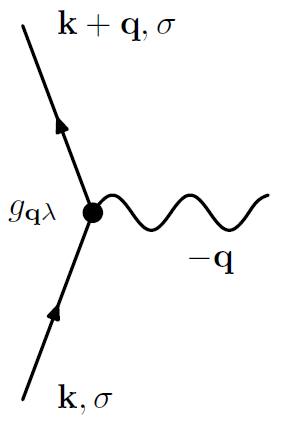
\includegraphics[width=0.25\textwidth]{immagini/diagramma_di_Feynman_2.png}
\end{figure}
\hspace{-0.6cm}Nel diagramma si rappresenta un elettrone che interagisce con il potenziale deformato. Diagrammaticamente questo corrisponde all'emissione o assorbimento di un fonone. Se un secondo elettrone interagisce con lo stesso fonone, il risultato complessivo è un'interazione efficace tra i due elettroni mediata dallo scambio del fonone.\\
Questa descrizione qualitativa può essere resa quantitativa introducendo un'interazione efficace tra elettroni che dipende dal momento del fonone e dalla frequenza:
\begin{equation}
   V_{\rm eff}(\vb{q},\omega)
   =|g_{\vb{q},\lambda}|^2 \frac{1}{\omega^2 - \omega_{\vb{q}}^2}
\end{equation}
Questa quantità risulta negativa quando $\omega < \omega_{\vb{q},\lambda}$, il che implica un'interazione attrattiva tra gli elettroni. Il coefficiente di accoppiamento segue la seguente dipendenza:
\begin{equation*}
   g_{\vb{q},\lambda}
   \propto \sqrt{\frac{m}{M}}
\end{equation*}
dove $m$ è la massa dell'elettrone e $M$ quella dell'isotopo. Questo fattore è tipicamente dell'ordine di $10^{-2}$, indicando che l'interazione è debole.\\
Prendiamo questa forma come punto di partenza. Bardeen, Cooper e Schrieffer introdussero una semplificazione importante: invece di considerare la dipendenza dal momento del fonone, si assume un'interazione efficace che dipende solo da una scala energetica caratteristica, la frequenza di Debye $\omega_D$, cioè la massima frequenza dei fononi:
\begin{equation*}
   V_{\rm eff}(\vb{q},\omega)
   =|g_{\rm eff}|^2 \frac{1}{\omega^2 - \omega_D^2}
\end{equation*}
Questo equivale a trascurare i dettagli microscopici dei singoli modi, mantenendo solo la scala energetica rilevante.\\
Poiché la superconduttività si manifesta a temperature $T < T_c$, la scala energetica associata è $k_B T_c$. Nei superconduttori convenzionali vale tipicamente $k_B T_c \ll \hbar \omega_D$, per cui si può trascurare la dipendenza dalla frequenza. L'interazione efficace diventa quindi:
\begin{equation*}
   V_{\rm eff}
   =-\frac{|g_{\rm eff}|^2}{\omega_D^2}
   \equiv - |V|^2
\end{equation*}
cioè una costante negativa.\\
A questo punto vogliamo scrivere l'hamiltoniana di interazione tra elettroni mediata dallo scambio di fononi. Nella teoria BCS si utilizzano operatori fermionici di creazione e annichilazione, $c^{\dag}$ e $c$, che rispettano le regole di anticommutazione per i fermioni. Poiché dipendono dal momento e dallo spin, li indichiamo con indici espliciti, cioè 
$c^{\dag}_{\vb{k},\sigma}$ e $c^{\vphantom{\dag}}_{\vb{k},\sigma}$, che sono rispettivamente l'operatore di creazione e annichilazione di un elettrone con momento $\vb{k}$ e spin $\sigma$.\\
Il processo descritto nel diagramma di Feynman è il seguente: due elettroni iniziali, $(\vb{k}_2,\sigma_2)$ e $(\vb{k}_1,\sigma_1)$, interagiscono scambiando un fonone, e dopo l'interazione diventano stati con momenti $\vb{k}_2 - \vb{q}$ e $\vb{k}_1 + \vb{q}$.\\
L'hamiltoniana deve quindi distruggere i due elettroni iniziali e creare i due finali:
\begin{equation}
   \hat{H}
   = - |V|^2 \sum_{\vb{k}} c^{\dag}_{\vb{k}_1 + \vb{q},\sigma_1} c^{\dag}_{\vb{k}_2 - \vb{q},\sigma_2} c^{\vphantom{\dag}}_{\vb{k}_1,\sigma_1} c^{\vphantom{\dag}}_{\vb{k}_2,\sigma_2}
   \label{eq:BCS_interaction_hamiltonian}
\end{equation}
Nel descrivere questo processo è fondamentale ricordare che, in un metallo, gli elettroni occupano gli stati fino all'energia di Fermi $E_F$. Di conseguenza, partecipano all'interazione solo gli elettroni vicini alla superficie di Fermi, cioè quelli per cui esistono stati disponibili in cui essere diffusi.
\begin{figure}[H]
   \centering
   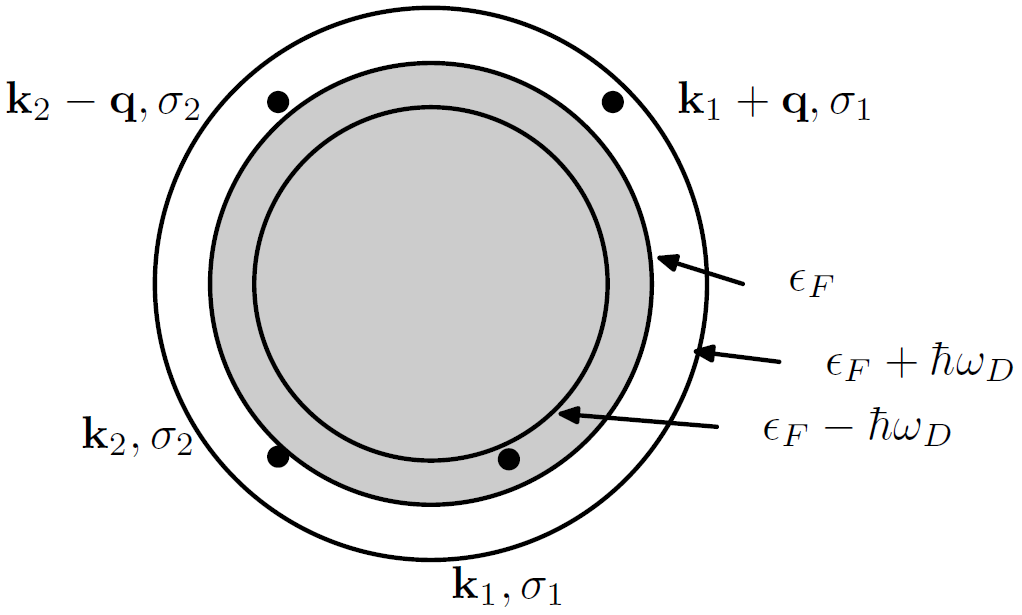
\includegraphics[width=0.5\textwidth]{immagini/superficie_di_Fermi.png}
\end{figure}
\hspace{-0.6cm}Gli elettroni coinvolti sono quindi confinati in una shell energetica attorno a $E_F$ di ampiezza dell'ordine di $\hbar \omega_D$: stati con energia inferiore a $E_F$ sono occupati, mentre quelli con energia maggiore sono disponibili.\\
Consideriamo quindi un elettrone con energia tra $E_F - \hbar \omega_D$ ed $E_F$, con momento $\vb{k}_1$. Dopo l'interazione con un fonone, esso può acquisire momento $\vb{k}_1 + \vb{q}$ ed essere diffuso in uno stato con energia superiore a $E_F$. Analogamente, un secondo elettrone vicino alla superficie di Fermi modifica il proprio stato.
\section{Problema di Cooper}
Vogliamo capire quale sia la struttura dello stato di due elettroni dopo che l'interazione attrattiva ha agito. In altre parole, vogliamo scrivere una funzione d'onda a due elettroni: questo è precisamente il cosiddetto \emph{problema di Cooper}. Esso consiste nello studiare lo stato di due elettroni che interagiscono tramite un'interazione attrattiva di qualche origine, e nel determinare quale relazione debba sussistere tra i loro momenti.\\
Supponiamo quindi di avere due elettroni con energia vicina al livello di Fermi. Quello che cerchiamo è la loro funzione d'onda, $\psi_0(\vb{r}_1,\vb{r}_2)$, a cui andrà poi aggiunta anche la parte di spin. Se i due elettroni hanno momenti $\vb{k}_1$ e $\vb{k}_2$, il loro momento totale è $\vb{K}=\vb{k}_1 + \vb{k}_2$.\\
Nel problema di Cooper, siamo interessati allo stato a energia minima di due elettroni sopra il mare di Fermi. Per argomenti generali,\sn{Il motivo per cui lo stato a energia minima ha momento totale nullo può essere compreso separando il moto dei due elettroni in moto del centro di massa e moto relativo. L'energia totale contiene infatti un contributo positivo associato al moto del centro di massa,
\begin{equation*}
   E=E_{\text{rel}} + \frac{\hbar^2 K^2}{4m}
\end{equation*}
dove $\vb{K}=\vb{k}_1 + \vb{k}_2$. Poiché il secondo termine è sempre positivo, l'energia è minima per $\vb{K}=0$, cioè quando i due elettroni hanno momenti opposti.} tale stato ha momento totale nullo, cioè
\begin{equation*}
   \vb{K}=\vb{k}_1 + \vb{k}_2=0
\end{equation*}
da cui segue che i due elettroni hanno momenti opposti:
\begin{equation*}
   \vb{k}_1=-\vb{k}_2\equiv \vb{k}
\end{equation*}
Di conseguenza, la parte spaziale della funzione d'onda può essere scritta come una sovrapposizione di stati con momenti opposti:
\begin{equation*}
   \psi_0(\vb{r}_1,\vb{r}_2)
   =\sum_{\vb{k}} g_{\vb{k}}\, e^{i \vb{k}\cdot \vb{r}_1} e^{-i \vb{k}\cdot \vb{r}_2}
\end{equation*}
Poiché gli elettroni sono fermioni, dobbiamo includere anche lo spin. Sappiamo che due spin $1/2$ possono combinarsi in uno stato di singoletto oppure in uno stato di tripletto. Nel primo caso la parte di spin è antisimmetrica, nel secondo è simmetrica.\\
Ricordiamo che lo stato totale di due fermioni deve essere complessivamente antisimmetrico rispetto allo scambio delle due particelle. Questo significa che possiamo avere una parte spaziale simmetrica moltiplicata per una parte di spin antisimmetrica, oppure una parte spaziale antisimmetrica moltiplicata per una parte di spin simmetrica.\\
Per capire la simmetria della parte spaziale, riscriviamo $\psi_0$ come
\begin{equation*}
   \begin{split}
      \psi_0(\vb{r}_1,\vb{r}_2)
      &=\sum_{\vb{k}} g_{\vb{k}}\, e^{i\vb{k}\cdot(\vb{r}_1-\vb{r}_2)}
      \\
      &=\sum_{\vb{k}} g_{\vb{k}}
      \Bigl\{
      \cos\bigl[\vb{k}\cdot(\vb{r}_1-\vb{r}_2)\bigr]
      + i \sin\bigl[\vb{k}\cdot(\vb{r}_1-\vb{r}_2)\bigr]
      \Bigr\}
   \end{split}
\end{equation*}
La parte con il coseno è simmetrica per scambio $\vb{r}_1 \leftrightarrow \vb{r}_2$, mentre quella con il seno è antisimmetrica. Quindi lo stato totale può essere o del tipo\mn{Nelle espressioni che seguono $\alpha_1$ indica lo stato di spin up della particella 1, mentre $\beta_1$ indica il suo stato di spin down, e analogamente per la particella 2.}
\begin{equation*}
   \psi_0(\vb{r}_1,\sigma_1;\vb{r}_2,\sigma_2)
   =\sum_{\vb{k}} g_{\vb{k}}
   \cos\bigl[\vb{k}\cdot(\vb{r}_1-\vb{r}_2)\bigr]
   \,(\alpha_1\beta_2-\beta_1\alpha_2)
\end{equation*}
oppure del tipo
\begin{equation*}
   \psi_0(\vb{r}_1,\sigma_1;\vb{r}_2,\sigma_2)
   =\sum_{\vb{k}} g_{\vb{k}}
   \sin\bigl[\vb{k}\cdot(\vb{r}_1-\vb{r}_2)\bigr]
   \times
   \begin{Bmatrix}
      \alpha_1\alpha_2\\[0.1cm]
      \frac{1}{\sqrt{2}}(\alpha_1\beta_2+\beta_1\alpha_2)\\[0.1cm]
      \beta_1\beta_2
   \end{Bmatrix}
\end{equation*}
Stiamo descrivendo un'interazione attrattiva tra due elettroni, quindi un'interazione che tende a portarli vicini tra loro. In questa situazione, lo stato favorito è il primo, cioè quello con parte spaziale simmetrica e parte di spin antisimmetrica. Infatti, se l'interazione è attrattiva, gli elettroni devono avere probabilità non nulla di trovarsi a piccola distanza relativa. La probabilità di trovare i due elettroni molto vicini è determinata dalla parte spaziale della funzione d'onda per $\vb{r}_1 \simeq \vb{r}_2$. In tal caso, la parte con il seno si annulla, mentre quella con il coseno resta diversa da zero. Di conseguenza, lo stato con singoletto di spin è quello energeticamente favorito. La funzione d'onda della coppia risulta quindi
\begin{equation}
   \psi_0
   =\sum_{\vb{k}} g_{\vb{k}}
   \cos\bigl[\vb{k}\cdot(\vb{r}_1-\vb{r}_2)\bigr]
   (\alpha_1\beta_2-\beta_1\alpha_2)
   \label{eq:cooper_pair_wavefunction}
\end{equation}
Questo è ciò che si chiama una \emph{coppia di Cooper}: una combinazione speciale di due elettroni con momenti opposti e spin opposti.\\
Una volta identificato questo stato, vogliamo verificare se esso abbia effettivamente energia più bassa rispetto a due elettroni non accoppiati. Per farlo, dobbiamo calcolare il valore medio dell'hamiltoniana totale nello stato $\ket*{\psi_0}$.\\
L'hamiltoniana totale è
\begin{equation*}
   \hat{H}
   =\hat{H}_0 + \hat{V}
\end{equation*}
dove $\hat{H}_0$ è l'hamiltoniana degli elettroni liberi:
\begin{equation}
   \hat{H}_0
   =\sum_{\vb{k},\sigma} \varepsilon_{\vb{k}} c^{\dag}_{\vb{k},\sigma} c^{\vphantom{\dag}}_{\vb{k},\sigma}
   \label{eq:free_electron_hamiltonian}
\end{equation}
con
\begin{equation*}
   \varepsilon_{\vb{k}}
   =\frac{\hbar^2 k^2}{2m}
\end{equation*}
mentre $\hat{V}$ rappresenta l'interazione attrattiva.\\
Cominciamo calcolando il valore medio di $\hat{H}_0$. Introduciamo la notazione di Dirac e indichiamo con $\ket*{\vb{k}}$ lo stato di coppia con momenti opposti $\vb{k}$ e $-\vb{k}$.\mn{Più precisamente, lo stato sarebbe qualcosa del tipo $\ket*{\vb{k},\uparrow;-\vb{k},\downarrow}$, e la sua parte spaziale è proporzionale a $\cos[\vb{k}\cdot(\vb{r}_1-\vb{r}_2)]$.} Poiché $\hat{H}_0$ non agisce sullo spin, nel calcolare tale valor medio possiamo concentrarci solo sulla parte orbitale. Si ha:
\begin{equation*}
   \begin{split}
      \expval*{\hat{H}_0}
      &=
      \Bigl(\sum_{\vb{k}'} g_{\vb{k}'}^* \bra*{\vb{k}'}\Bigr)
      \hat{H}_0
      \Bigl(\sum_{\vb{k}} g^{\vphantom{*}}_{\vb{k}} \ket*{\vb{k}}\Bigr)
      \\
      &=
      \sum_{\vb{k},\vb{k}'} g^*_{\vb{k}'} g^{\vphantom{*}}_{\vb{k}}
      \mel*{\vb{k}'}{\hat{H}_0}{\vb{k}}
   \end{split}
\end{equation*}
Esplicitiamo il termine $\mel*{\vb{k}'}{\hat{H}_0}{\vb{k}}$:
\begin{equation*}
   \mel*{\vb{k}'}{\hat{H}_0}{\vb{k}}
   =
   \sum_{\vb{k}'',\sigma} \varepsilon_{\vb{k}''}
   \mel*{\vb{k}'}{c^{\dag}_{\vb{k}'',\sigma} c^{\vphantom{\dag}}_{\vb{k}'',\sigma}}{\vb{k}}
\end{equation*}
L'operatore $c^{\dag}_{\vb{k}'',\sigma} c^{\vphantom{\dag}}_{\vb{k}'',\sigma}$ conta il numero di elettroni con momento $\vb{k}''$ e spin $\sigma$. Quando agisce su uno stato di coppia, dà contributo solo se quel momento e quello spin sono presenti nello stato, cioè
\begin{equation*}
   c^{\dag}_{\vb{k}'',\sigma} c^{\vphantom{\dag}}_{\vb{k}'',\sigma}
   \ket{\vb{k},\uparrow;\,-\vb{k},\downarrow}
   =
   \begin{cases}
      \ket{\vb{k},\uparrow;\,-\vb{k},\downarrow} 
      & \text{se } (\vb{k}'',\sigma)=(\vb{k},\uparrow)\ \text{o}\ (-\vb{k},\downarrow)\\[0.1cm]
      0 & \text{altrimenti}
   \end{cases}
\end{equation*}
Nel nostro caso lo stato contiene due elettroni, uno in $(\vb{k},\uparrow)$ e uno in $(-\vb{k},\downarrow)$, quindi l'energia libera totale della coppia è semplicemente
\begin{equation*}
   \varepsilon_{\vb{k}} + \varepsilon_{-\vb{k}}
   =2\varepsilon_{\vb{k}}
\end{equation*}
poiché $\varepsilon_{\vb{k}}=\varepsilon_{-\vb{k}}$. Ne segue che
\begin{equation*}
   \mel*{\vb{k}'}{\hat{H}_0}{\vb{k}}
   =2\varepsilon_{\vb{k}} \braket*{\vb{k}'}{\vb{k}}
   =2\varepsilon_{\vb{k}}\,\delta_{\vb{k}',\vb{k}}
\end{equation*}
Pertanto
\begin{equation*}
   \expval*{\hat{H}_0}
   =\sum_{\vb{k}} |g_{\vb{k}}|^2\, 2\varepsilon_{\vb{k}}
\end{equation*}
Passiamo ora al valore medio dell'interazione:
\begin{equation*}
   \expval*{\hat{V}}
   =\sum_{\vb{k},\vb{k}'} g_{\vb{k}'}^* g^{\vphantom{*}}_{\vb{k}}
   \mel*{\vb{k}'}{\hat{V}}{\vb{k}}
   =\sum_{\vb{k},\vb{k}'} g_{\vb{k}'}^* g^{\vphantom{*}}_{\vb{k}}\, V_{\vb{k}',\vb{k}}
\end{equation*}
dove $V_{\vb{k}',\vb{k}}=\mel*{\vb{k}'}{\hat{V}}{\vb{k}}$ è l'elemento di matrice dell'interazione tra due stati di coppia diversi.\\
Vogliamo determinare la condizione di equilibrio, cioè la condizione di minima energia. Consideriamo quindi
\begin{equation*}
   \expval{H_0 + V}
   =
   E \braket{\psi}{\psi}
\end{equation*}
Per quanto riguarda il secondo membro, abbiamo
\begin{equation*}
   \braket{\psi}{\psi}
   =
   \Bigl(\sum_{\vb{k}'} g_{\vb{k}'}^* \bra*{\vb{k}'}\Bigr)
   \Bigl(\sum_{\vb{k}} g^{\vphantom{*}}_{\vb{k}} \ket*{\vb{k}}\Bigr)
   =
   \sum_{\vb{k}} |g_{\vb{k}}|^2
\end{equation*}
Utilizzando i risultati precedenti otteniamo
\begin{equation*}
   \sum_{\vb{k}} |g_{\vb{k}}|^2 \, 2 \varepsilon_{\vb{k}}
   +
   \sum_{\vb{k},\vb{k}'} g_{\vb{k}'}^* g^{\vphantom{*}}_{\vb{k}} V^{\vphantom{*}}_{\vb{k}',\vb{k}}
   =
   E \sum_{\vb{k}} |g_{\vb{k}}|^2
\end{equation*}
Portando tutti i termini al primo membro:
\begin{equation*}
   \sum_{\vb{k}} |g_{\vb{k}}|^2 (2 \varepsilon_{\vb{k}} - E)
   +
   \sum_{\vb{k},\vb{k}'} g_{\vb{k}'}^* g^{\vphantom{*}}_{\vb{k}} V^{\vphantom{*}}_{\vb{k}',\vb{k}}
   = 0
\end{equation*}
Raccogliendo la somma su $\vb{k}$, possiamo scrivere
\begin{equation*}
   \sum_{\vb{k}}
   \Big\{
      |g_{\vb{k}}|^2 (2 \varepsilon_{\vb{k}} - E)
      +
      \sum_{\vb{k}'} g_{\vb{k}'}^* g^{\vphantom{*}}_{\vb{k}} \, V_{\vb{k}',\vb{k}}
   \Big\}
   = 0
\end{equation*}
Affinché questa relazione sia soddisfatta, imponiamo che il termine tra parentesi graffe si annulli per ogni $\vb{k}$:
\begin{equation*}
   |g_{\vb{k}}|^2 (2 \varepsilon_{\vb{k}} - E)
   +
   \sum_{\vb{k}'} g_{\vb{k}'}^* g^{\vphantom{*}}_{\vb{k}} \, V_{\vb{k}',\vb{k}}
   = 0
\end{equation*}
Mettendo in evidenza $g_{\vb{k}}$, otteniamo
\begin{equation*}
   g_{\vb{k}}
   \Big[
      g_{\vb{k}}^* (2 \varepsilon_{\vb{k}} - E)
      +
      \sum_{\vb{k}'} g_{\vb{k}'}^* V_{\vb{k}',\vb{k}}
   \Big]
   = 0
\end{equation*}
Scartando la soluzione banale $g_{\vb{k}} = 0$, si ha
\begin{equation*}
   g_{\vb{k}}^* (2 \varepsilon_{\vb{k}} - E)
   +
   \sum_{\vb{k}'} g_{\vb{k}'}^* V_{\vb{k}',\vb{k}}
   = 0
\end{equation*}
Prendendo il complesso coniugato:
\begin{equation*}
   g_{\vb{k}} (2 \varepsilon_{\vb{k}} - E)
   +
   \sum_{\vb{k}'} g_{\vb{k}'} V_{\vb{k}',\vb{k}}
   = 0
\end{equation*}
Da cui si può scrivere
\begin{equation*}
   g_{\vb{k}}
   =
   - \frac{\sum_{\vb{k}'} g_{\vb{k}'} V_{\vb{k}',\vb{k}}}{2 \varepsilon_{\vb{k}} - E}
\end{equation*}
In generale l'elemento di matrice $V_{\vb{k},\vb{k}'}$ dipende da $\vb{k}$ e $\vb{k}'$, perché deriva dall'interazione efficace mediata dai fononi\mn{\cite{Tinkham} $V_{\vb{k},\vb{k}'}$ descrive la forza dell'interazione per lo scattering di una coppia di elettroni con momenti $(\vb{k}',-\vb{k}')$ in una coppia con momenti $(\vb{k},-\vb{k})$.}. Tuttavia, Cooper fece l'assunzione semplificatrice che tale interazione sia costante all'interno della shell energetica rilevante:
\begin{equation*}
   V_{\vb{k},\vb{k}'}=V
   \qq{,}
   V<0
\end{equation*}
Questa è la cosiddetta \emph{assunzione di Cooper}. L'equazione precedente diventa allora
\begin{equation*}
   g_{\vb{k}}
   =-V\,\frac{\sum_{\vb{k}'} g_{\vb{k}'}}{2\varepsilon_{\vb{k}}-E}
\end{equation*}
Sommiamo ora su tutti i valori di $\vb{k}$:
\begin{equation*}
   \sum_{\vb{k}} g_{\vb{k}}
   =-V \sum_{\vb{k}} \frac{\sum_{\vb{k}'} g_{\vb{k}'}}{2\varepsilon_{\vb{k}}-E}
\end{equation*}
Poiché il fattore $\sum_{\vb{k}'} g_{\vb{k}'}$ è comune, si semplifica e si ottiene:
\begin{equation*}
   1
   =-V \sum_{\vb{k}} \frac{1}{2\varepsilon_{\vb{k}}-E}
\end{equation*}
Poiché la somma va estesa solo agli stati disponibili al di sopra del livello di Fermi, si ha
\begin{equation*}
   1
   =-V \sum_{k \ge k_F}
   \frac{1}{2\varepsilon_{\vb{k}}-E}
\end{equation*}
La sommatoria può essere sostituita con un integrale introducendo la densità degli stati. La shell energetica al di sopra del livello di Fermi che dobbiamo considerare è quella determinata dalla frequenza di Debye:
\begin{equation*}
   -\frac{1}{V}
   =\int_{E_F}^{E_F+\hbar\omega_D}
   \dd{\varepsilon}\,
   N(\varepsilon)\,
   \frac{1}{2\varepsilon-E}
\end{equation*}
Se la densità degli stati viene approssimata con il suo valore al livello di Fermi, $N(E_F)$, si ha
\begin{equation*}
   -\frac{1}{V}
   =N(E_F)\int_{E_F}^{E_F+\hbar\omega_D} \dd{\varepsilon} \frac{1}{2\varepsilon-E}
\end{equation*}
L'integrale dà
\begin{equation*}
   -\frac{1}{V}
   =\frac{N(E_F)}{2}
   \ln\qty[ \frac{2E_F+2\hbar\omega_D-E}{2E_F-E} ]
\end{equation*}
Esponenziando entrambi i membri:
\begin{equation*}
   e^{-2/[V N(E_F)]}
   =\frac{2E_F+2\hbar\omega_D-E}{2E_F-E}
   =1+\frac{2\hbar\omega_D}{2E_F-E}
\end{equation*}
Da cui, con qualche passaggio algebrico,
\begin{equation*}
   E
   =2E_F-\frac{2\hbar\omega_D}{e^{-2/[V N(E_F)]}-1}
\end{equation*}
Ponendo $V=-|V|$, cioè esplicitando che l'interazione è attrattiva, si ottiene
\begin{equation*}
   E
   =2E_F-\frac{2\hbar\omega_D}{e^{2/[|V|N(E_F)]}-1}
\end{equation*}
Poiché $|V|$ è piccolo,\mn{\cite{Tinkham} In gran parte dei superconduttori convenzionali si trova che $N(E_F) |V|<0.3$. Ciò permette di utilizzare la cosiddetta approssimazione di accoppiamento debole, valida per $N(E_F) |V| \ll 1$.} l'esponenziale è molto grande rispetto a $1$. Possiamo quindi fare l'approssimazione:
\begin{equation}
   E
   \simeq
   2E_F-2\hbar\omega_D\, e^{-2/[|V|N(E_F)]}
   \label{eq:energia_cooper}
\end{equation}
Questa espressione mostra che l'energia della coppia di Cooper è minore di $2E_F$, cioè minore dell'energia che avrebbero due elettroni indipendenti al livello di Fermi. Questo significa che, in presenza di un'interazione attrattiva, per quanto debole, i due elettroni preferiscono formare una coppia con momenti opposti e spin opposti.\\
Il punto fondamentale è che la correzione energetica non è una piccola correzione perturbativa proporzionale a $V$, ma ha una dipendenza esponenziale in $1/|V|$. Questo è un effetto essenzialmente non perturbativo, ed è uno degli aspetti più profondi del problema di Cooper.\sn{\cite{Tinkham} Si noti che che la forma dell'energia di legame non è analitica in $V=0$, cioè non può essere espansa in potenze di $V$. Di conseguenza, non può essere ottenuta tramite teoria perturbativa, un fatto che ha notevolmente ritardato la genesi della teoria.}.\\
Facciamo adesso alcuni commenti sulla struttura dello stato dato dall'\eqrefcustom{eq:cooper_pair_wavefunction}. I coefficienti $g_{\vb{k}}$ dipendono solo da $k^2$, e quindi non selezionano alcuna direzione privilegiata nello spazio. Questo corrisponde a un accoppiamento di tipo $s$, cioè a una simmetria sferica della coppia.\\
Un altro aspetto importante riguarda l'estensione spaziale della coppia. Essa può essere stimata a partire dal momento della coppia, che è legata alla velocità di Fermi $v_F$ in quanto gli elettroni coinvolti hanno energia vicina a $E_F$. D'altra parte, la scala energetica rilevante è data da $k_B T_c$, che è la scala energetica associata alla transizione superconduttiva. Si ottiene così una lunghezza caratteristica
\begin{equation*}
   \xi_0
   =\frac{\hbar v_F}{k_B T_c}
\end{equation*}
Questa quantità è dell'ordine della lunghezza di coerenza ed è tipicamente molto grande, dell'ordine di $10^4$\;\AA, se si usano valori tipici $v_F\sim 10^8\;\mathrm{cm/s}$ e $T_c\sim 10\;\mathrm{K}$.\\
Questo ci dice che la distanza media tra i due elettroni che formano una coppia di Cooper è molto maggiore della distanza interparticellare media. È importante sottolinearlo, perché si potrebbe essere portati a immaginare una coppia di Cooper come due elettroni molto vicini che si muovono insieme quasi come due palline legate. In realtà non è così: la coppia è un oggetto quantistico esteso. I due elettroni sono fortemente correlati, ma non sono necessariamente vicini nello spazio in senso classico.
\section{Stato fondamentale BCS}
A questo punto vogliamo capire quali siano le conseguenze delle proprietà dello stato di coppia di Cooper in un sistema reale, cioè in un solido. In altre parole, non consideriamo più una singola coppia di elettroni, ma un metallo in cui è presente un'interazione attrattiva tra molti elettroni. Questo ci porterà a determinare la struttura dello stato fondamentale nella teoria BCS.\\
Il punto cruciale è che abbiamo a che fare con uno stato a molti corpi di fermioni, quindi è necessario introdurre un certo formalismo matematico per determinarne la struttura.\\
Il punto di partenza è l'Hamiltoniana del sistema, che è composta da una parte di elettroni liberi e da una parte che descrive l'interazione, la quale assume la forma che abbiamo derivato considerando l'interazione mediata dai fononi.\\
Abbiamo assunto che l'interazione non dipenda da $\vb{k}$ e che sia negativa, a condizione che l'energia coinvolta sia minore dell'energia di Debye, che rappresenta la scala energetica rilevante.\\
Possiamo scrivere esplicitamente questa interazione utilizzando gli operatori fermionici di creazione e annichilazione che, come abbiamo visto, portano alla forma data nell'\eqrefcustom{eq:BCS_interaction_hamiltonian}, se consideriamo semplicemente i processi in cui due elettroni vengono diffusi tramite l'interazione con un fonone di momento generico.\\
Nel complesso, l'interazione comporta l'annichilazione di due elettroni e la creazione di altri due elettroni, ciascuno con momento diverso, ma in modo tale che il momento totale sia conservato. Inoltre, lo spin non è coinvolto nell'interazione, in quanto non viene modificato.
\subsection{Hamiltoniana di pairing}
Partiamo dallo scrivere quella che viene chiamata Hamiltoniana di pairing, cioè una Hamiltoniana che descrive questo meccanismo di interazione.\\
In essa abbiamo una parte di elettroni liberi, data da
\begin{equation*}
   H_0
   =\sum_{\vb{k},\sigma} \varepsilon(\vb{k}) c^{\dag}_{\vb{k},\sigma} c^{\vphantom{\dag}}_{\vb{k},\sigma}
\end{equation*}
e una parte di interazione data da\mn{Si presti attenzione al fatto che stiamo usando la notazione
\begin{equation*}
   -|V| \to \frac{V}{2}
\end{equation*}
}
\begin{equation*}
   H_I
   =\frac{V}{2} \sum_{\vb{k},\vb{k}',\vb{q}} \sum_{\sigma,\sigma'} 
   c^{\dag}_{\vb{k + q},\sigma} 
   c^{\dag}_{\vb{k' - q},\sigma'} 
   c^{\vphantom{\dag}}_{\vb{k}',\sigma'} 
   c^{\vphantom{\dag}}_{\vb{k},\sigma}
\end{equation*}
Poiché queste interazioni coinvolgono coppie di elettroni con combinazioni di momento e spin del tipo $(\vb{k},\uparrow)$ e $(-\vb{k},\downarrow)$, nella somma possiamo imporre che $\vb{k}'=-\vb{k}$ e $\sigma'=-\sigma$. In questo modo, nel termine di interazione non è più necessario sommare su $\vb{k}'$ e su $\sigma'$:
\begin{equation*}
   H_I
   =\frac{V}{2} \sum_{\vb{k},\vb{q}} \sum_{\sigma} 
   c^{\dag}_{\vb{k + q},\sigma} 
   c^{\dag}_{-\vb{k - q},-\sigma} 
   c^{\vphantom{\dag}}_{-\vb{k},-\sigma} 
   c^{\vphantom{\dag}}_{\vb{k},\sigma}
\end{equation*}
Se ora esplicitiamo le combinazioni di momento e spin che contribuiscono all'interazione, otteniamo\mn{Stiamo semplicemente introducendo il cambio di variabile $\vb{k}'=\vb{k}+\vb{q}$, di modo che il termine di interazione descriva lo scattering di una coppia $(\vb{k},-\vb{k})$ in una coppia $(\vb{k}',-\vb{k}')$.}
\begin{equation*}
   H_I
   = V \sum_{\vb{k},\vb{k}'} 
   c^{\dag}_{\vb{k'},\uparrow} 
   c^{\dag}_{-\vb{k'},\downarrow} 
   c^{\vphantom{\dag}}_{-\vb{k},\downarrow} 
   c^{\vphantom{\dag}}_{\vb{k},\uparrow}
\end{equation*}
Qui abbiamo introdotto un fattore 2, poiché $\sigma$ può assumere i valori $\uparrow$ o $\downarrow$ e, dato che l'interazione non dipende dallo spin, possiamo fissare un particolare ordine degli operatori (ad esempio $\uparrow, \downarrow, \downarrow, \uparrow$), tenendo conto che le altre combinazioni danno contributi equivalenti.\\
A questo punto introduciamo il cosiddetto operatore di creazione di una coppia di Cooper $Z^{\dag}_{\vb{k}}$, definito come
\begin{equation*}
   Z^{\dag}_{\vb{k}}
   =c^{\dag}_{\vb{k},\uparrow} c^{\dag}_{-\vb{k},\downarrow}
\end{equation*}
Si tratta quindi di un operatore composto da due operatori di creazione: uno per un elettrone $(\vb{k},\uparrow)$ e l'altro per un elettrone $(-\vb{k},\downarrow)$. Possiamo riscrivere il termine di interazione in funzione di questo operatore come
\begin{equation*}
   H_I
   = V \sum_{\vb{k}'} Z^{\dag}_{\vb{k}'} \sum_{\vb{k}} Z^{\vphantom{\dag}}_{\vb{k}}
   =\frac{1}{V} \hat{\Delta}^{\dag} \hat{\Delta}
\end{equation*}
dove abbiamo introdotto l'operatore
\begin{equation*}
   \hat{\Delta} \equiv V \sum_{\vb{k}} Z_{\vb{k}}
\end{equation*}
\subsection{Funzione d'onda di prova}
Ora dobbiamo capire, a partire da questo tipo di interazione, quale sia la struttura dello stato fondamentale. Il procedimento che utilizziamo è un procedimento variazionale: ciò significa che scriviamo una funzione d'onda di prova, introduciamo alcuni coefficienti e poi cerchiamo il minimo del valor medio dell'Hamiltoniana.\\
Per costruire la funzione d'onda di prova partiamo da ciò che già conosciamo, cioè il comportamento di un metallo in assenza di superconduttività. Infatti, dobbiamo partire da una funzione d'onda che, nel limite in cui l'interazione viene spenta, si riduca allo stato fondamentale degli elettroni liberi.\\
Lo stato fondamentale di un gas di Fermi non interagente, essendo costituito da elettroni liberi che occupano tutti gli stati con momento fino al momento di Fermi, può essere scritto come
\begin{equation*}
   \ket*{g_{\rm free}}
   =\prod_{k \leq k_F} Z^{\dag}_{\vb{k}} \ket*{0}
\end{equation*}
In questo modo consideriamo tutti gli stati con diversi valori di $k$ in forma di prodotto. Nulla vieta di raggruppare gli stati a due elettroni e scriverli come prodotto di coppie (dove con coppie non intendiamo ancora le coppie di Cooper, ma semplicemente coppie di elettroni).\\
Ricordiamo che l'operatore $Z^{\dag}_{\vb{k}}$ crea un elettrone $(\vb{k},\uparrow)$ e uno $(-\vb{k},\downarrow)$; quindi, se consideriamo per tutti i valori di $k<k_F$ uno stato del tipo
\begin{equation*}
   \prod_{k<k_F} \ket*{\vb{k},\uparrow} \hspace{-0.17cm} \ket*{-\vb{k},\downarrow}
\end{equation*}
otteniamo uno stato che descrive tutti gli elettroni liberi con momento minore di $k_F$.\\
Possiamo ora immaginare di costruire delle sovrapposizioni. In generale, sappiamo che in meccanica quantistica una particella può trovarsi in una sovrapposizione di stati. Se un sistema può essere negli stati $\ket*{a}$ e $\ket*{b}$, può anche trovarsi nello stato $c_a \ket*{a} + c_b \ket*{b}$, dove $\ket*{a}$ e $\ket*{b}$ sono autostati. Qui però vogliamo costruire una sovrapposizione di tipo particolare: ci chiediamo infatti se sia possibile costruire sovrapposizioni di stati con diverso numero di particelle, cioè stati del tipo
\begin{equation*}
   \ket*{\psi}=u \ket*{0_{\vb{k}}} + \nu \ket*{2_{\vb{k}}}
\end{equation*}
Questo stato rappresenta una sovrapposizione di uno stato con zero particelle di momento $\vb{k}$ e uno stato con due particelle. Precisiamo che lo stato $\ket*{2_{\vb{k}}}$ è definito come
\begin{equation*}
   \ket*{2_{\vb{k}}}
   =Z^{\dag}_{\vb{k}} \ket*{0_{\vb{k}}}
\end{equation*}
cioè come l'azione dell'operatore di creazione di coppia con momento $\vb{k}$ sullo stato vuoto. Si tratta quindi di uno stato con due elettroni aventi momenti opposti e spin opposti. In altre parole, il simbolo “2” indica il numero di elettroni, mentre $\vb{k}$ identifica il valore del momento associato alla coppia.\\
Lo stato che abbiamo scritto è una sovrapposizione quantistica di due stati, ma con una differenza rispetto ai casi usuali: si tratta infatti di una sovrapposizione di stati con numero diverso di particelle. Vedremo che la struttura dello stato fondamentale BCS è proprio di questo tipo:
\begin{equation}
   \ket*{g_s}
   =\prod_{\vb{k}} \bigl( u_{\vb{k}} \ket*{0_{\vb{k}}} + \nu_{\vb{k}} \ket{2_{\vb{k}}} \bigr)
   \label{eq:BCS_trial_wavefunction}
\end{equation}
Questo stato è quindi il prodotto, su tutti i valori di $\vb{k}$,\mn{Con “tutti i valori di $\vb{k}$” si intendono sia quelli minori che maggiori di $k_F$.} di sovrapposizioni di stati con zero e due particelle. In altre parole, la funzione d'onda di prova che utilizzeremo per minimizzare il valor medio dell'Hamiltoniana è costruita come prodotto, su tutti i $\vb{k}$, di sovrapposizioni di stati con zero e due elettroni, dove i due elettroni sono quelli creati dall'operatore di coppia.\\
Consideriamo una sovrapposizione di questi due stati perché, come abbiamo visto, l'interazione attrattiva ha la forma di un termine che distrugge tutte le possibili coppie moltiplicato per un termine che crea tutte le possibili coppie, cioè $\hat{\Delta}^{\dag}\hat{\Delta}$. Dalla struttura dell'interazione nasce quindi l'idea di cercare stati di questo tipo.\\
Un punto importante da osservare è che uno stato di questa forma non ha un numero fissato di particelle, poiché in generale contiene contributi con diverso numero di elettroni.\\
A questo punto dobbiamo calcolare il valor medio dell'Hamiltoniana, includendo il termine di interazione. Il primo passo consiste nello scrivere esplicitamente questo valor medio sullo stato di prova, mentre il secondo passo consiste nel minimizzarlo rispetto ai coefficienti, che sono proprio $u_{\vb{k}}$ e $\nu_{\vb{k}}$.\\
Prima di procedere, facciamo un'osservazione: in assenza di interazione non devono comparire stati $\ket*{2_{\vb{k}}}$ per $k > k_F$, quindi i coefficienti $\nu_{\vb{k}}$ devono essere legati alla presenza dell'interazione. Vogliamo allora che, nel limite in cui $V \to 0$, lo stato di prova $\ket*{g_s}$ si riduca allo stato fondamentale degli elettroni liberi $\ket*{g_{\rm free}}$.\\
Ciò richiede che, per $V \to 0$,
\begin{equation*}
   u_{\vb{k}}
   =
   \begin{cases}
      0 & \text{per }k<k_F\\
      1 & \text{per }k>k_F
   \end{cases}
   \qq{,}
   \nu_{\vb{k}}
   =
   \begin{cases}
      1 & \text{per }k<k_F\\
      0 & \text{per }k>k_F
   \end{cases}
\end{equation*}
In questo modo, per $k<k_F$ le coppie risultano occupate, mentre per $k>k_F$ risultano vuote, riproducendo il mare di Fermi degli elettroni liberi.\\
Un'ulteriore condizione da imporre è la normalizzazione degli stati, che richiede
\begin{equation}
   |u_{\vb{k}}|^2 + |\nu_{\vb{k}}|^2
   =1
   \label{eq:BCS_normalization_condition}
\end{equation}
\subsection{Box di Nambu}
Lo stato dato dall'\eqrefcustom{eq:BCS_trial_wavefunction} è uno stato prodotto che coinvolge, per ogni $\vb{k}$, una sovrapposizione degli stati $\ket*{0_{\vb{k}}}$ e $\ket*{2_{\vb{k}}}$. Questo significa che la funzione d'onda di prova è fattorizzata rispetto ai diversi valori di $\vb{k}$: ogni coppia $(\vb{k}, -\vb{k})$ è descritta da una sovrapposizione indipendente, senza correlazioni dirette tra sottospazi con momenti diversi.\\
Torniamo ora ai due elettroni che formano queste sovrapposizioni: uno è nello stato $(\vb{k},\uparrow)$ e l'altro in $(-\vb{k},\downarrow)$. Considerando questi due stati, si possono avere diverse configurazioni possibili: nessun elettrone, entrambi gli elettroni, oppure un solo elettrone in uno dei due stati e nessuno nell'altro. In altre parole, lo spazio degli stati accessibili è costituito da quattro configurazioni:
\begin{equation*}
   \begin{array}{ll}
      \ket*{0}=\ket*{0_{\vb{k},\uparrow}; 0_{-\vb{k},\downarrow}} 
      & \ket*{2}=\ket*{1_{\vb{k},\uparrow}; 1_{-\vb{k},\downarrow}}\\[0.2cm]
      \ket*{+}=\ket*{1_{\vb{k},\uparrow}; 0_{-\vb{k},\downarrow}} 
      & \ket*{-}=\ket*{0_{\vb{k},\uparrow}; 1_{-\vb{k},\downarrow}}
   \end{array}
\end{equation*}
Questo sottospazio dello spazio di Hilbert totale, associato a un dato $\vb{k}$, prende il nome di \textit{box di Nambu}. Un box di Nambu consiste quindi nel considerare due livelli elettronici, $(\vb{k},\uparrow)$ e $(-\vb{k},\downarrow)$, e tutte le possibili occupazioni: zero, uno o due elettroni. Lo stato $\ket*{0}$ corrisponde all'assenza di elettroni in entrambi i livelli, lo stato $\ket*{2}$ alla presenza di entrambi gli elettroni, mentre $\ket*{+}$ e $\ket*{-}$ rappresentano gli stati con un solo elettrone. Si tratta quindi di uno spazio di Fock a quattro dimensioni. Vedremo che lavorare in termini di box di Nambu è particolarmente conveniente per trattare la funzione d'onda di prova.\\
Consideriamo ora l'azione dell'operatore di creazione di coppia in questo box.
\begin{figure}[H]
   \centering
   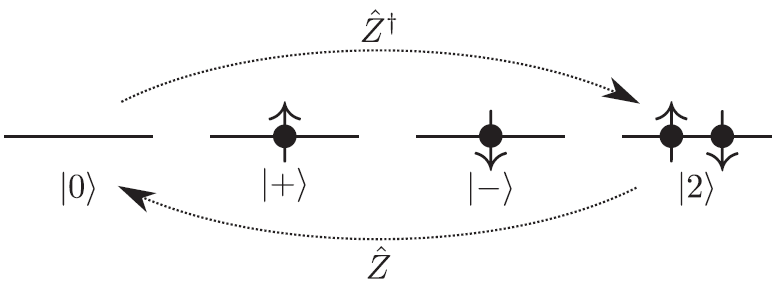
\includegraphics[width=0.6\textwidth]{immagini/azione_Zk_Nambu_box.png}
\end{figure}
\hspace{-0.6cm}Esso trasforma $\ket*{0_{\vb{k}}}$ in $\ket*{2_{\vb{k}}}$, mentre non connette direttamente gli stati $\ket*{+}$ e $\ket*{-}$, poiché è composto da due operatori di creazione. Di conseguenza, per quanto riguarda l'interazione, possiamo limitarci al sottospazio bidimensionale generato da $\ket*{0_{\vb{k}}}$ e $\ket*{2_{\vb{k}}}$. Gli altri due stati non vengono considerati in questa fase, ma è importante ricordare che possono diventare rilevanti quando si studiano le eccitazioni rispetto allo stato fondamentale.\\
In questo sottospazio possiamo utilizzare la notazione dei sistemi a due livelli. In particolare si ha\mn{Si noti che la base è stata scelta in modo che $\ket*{2_{\vb{k}}}$ sia il primo vettore di base e $\ket*{0_{\vb{k}}}$ il secondo.}
\begin{equation*}
   \ket*{0_{\vb{k}}}
   =\begin{pmatrix}
      0\\
      1
   \end{pmatrix}
   \qq{;}
   \ket*{2_{\vb{k}}}
   =\begin{pmatrix}
      1\\
      0
   \end{pmatrix}
\end{equation*}
L'operatore di creazione di coppia assume quindi la forma matriciale
\begin{equation*}
   Z^{\dag}_{\vb{k}}
   =\begin{pmatrix}
      0 & 1 \\
      0 & 0
   \end{pmatrix}
\end{equation*}
infatti
\begin{equation*}
   Z^{\dag}_{\vb{k}} \ket*{0_{\vb{k}}}
   =
   \begin{pmatrix}
      0 & 1 \\
      0 & 0
   \end{pmatrix}
   \begin{pmatrix}
      0\\
      1
   \end{pmatrix}
   =
   \begin{pmatrix}
      1\\
      0
   \end{pmatrix}
   =\ket*{2_{\vb{k}}}
\end{equation*}
Analogamente, l'operatore di annichilazione di coppia è dato da
\begin{equation*}
   Z_{\vb{k}}
   =\begin{pmatrix}
      0 & 0 \\
      1 & 0
   \end{pmatrix}
\end{equation*}
Con questa descrizione, lo spazio di Fock a molti corpi può essere visto come prodotto diretto di tutti i box di Nambu, e la funzione d'onda di prova per lo stato fondamentale può essere riscritta come
\begin{equation}
   \ket*{g_s}
   =\prod_{\vb{k}} \bigl( u_{\vb{k}} + \nu_{\vb{k}} Z^{\dag}_{\vb{k}} \bigr) \ket*{0}
   \label{eq:BCS_trial_wavefunction_Nambu}
\end{equation}
dove ora $\ket*{0}$ rappresenta lo stato di vuoto globale, cioè lo stato senza elettroni per qualunque valore di $\vb{k}$ e dello spin.
\subsection{Energia dello stato fondamentale}
Passiamo ora al calcolo dell'energia dello stato fondamentale a partire dalla funzione d'onda di prova. Precisiamo che, poiché stiamo considerando uno stato in cui il numero di particelle non è fissato (essendo una sovrapposizione), nel metodo variazionale dobbiamo introdurre un moltiplicatore di Lagrange. In questo caso, tale vincolo è legato al numero medio di particelle, che entra attraverso il potenziale chimico.\\
Ciò significa che, partendo dall'Hamiltoniana totale, dobbiamo includere un termine che tenga conto del fatto che il numero di particelle non è fissato. Questo si realizza aggiungendo il termine $-\mu \hat{N}$, dove l'operatore numero è
\begin{equation*}
   \hat{N}
   =\sum_{\vb{k},\sigma} c^{\dag}_{\vb{k},\sigma} c^{\vphantom{\dag}}_{\vb{k},\sigma}
\end{equation*}
L'Hamiltoniana effettiva da utilizzare nel metodo variazionale diventa quindi
\begin{equation*}
   \hat{H}=\hat{H}_0 - \mu \hat{N} + \hat{H}_I
\end{equation*}
L'effetto di questo termine sulle energie è semplice, poiché ha la stessa struttura di $\hat{H}_0$ vista nell'\eqrefcustom{eq:free_electron_hamiltonian}. In pratica, introduce uno shift delle energie pari al potenziale chimico. Definendo
\begin{equation*}
   \xi_{\vb{k}}
   =\varepsilon(\vb{k}) - \mu
\end{equation*}
che rappresenta l'energia rispetto al livello di Fermi, possiamo riscrivere
\begin{equation*}
   \hat{H}_0 - \mu \hat{N}
   =\sum_{\vb{k},\sigma} \xi(\vb{k}) c^{\dag}_{\vb{k},\sigma} c^{\vphantom{\dag}}_{\vb{k},\sigma}
   =\sum_{\vb{k},\sigma} \xi(\vb{k}) \hat{n}_{\vb{k},\sigma}
\end{equation*}
dove $\hat{n}_{\vb{k},\sigma}=c^{\dag}_{\vb{k},\sigma} c^{\vphantom{\dag}}_{\vb{k},\sigma}$ è l'operatore numero.\\
Il primo passo consiste nel calcolare il numero medio di particelle sullo stato di prova, cioè $\expval*{\hat{N}}$; il secondo passo è valutare $\expval*{(\hat{N} - \expval*{\hat{N}})^2}$; senza entrare nei dettagli del calcolo, si trova che la deviazione quadratica media
\begin{equation*}
   \delta N_{\rm rms}
   =\sqrt{\big\langle \bigl( \hat{N} - \expval*{\hat{N}} \bigr)^2 \big\rangle}
\end{equation*}
scala come la radice quadrata del numero medio di particelle. Di conseguenza,
\begin{equation*}
   \frac{\delta N_{\rm rms}}{\expval*{\hat{N}}}
   \propto \frac{\sqrt{N}}{N}
   =\frac{1}{\sqrt{N}}
\end{equation*}
Poiché $N$ è il numero medio di elettroni nel sistema ed è quindi macroscopicamente grande, questa quantità è molto piccola. Questo significa che, pur considerando uno stato in cui il numero di particelle non è fissato, le fluttuazioni relative del numero di particelle sono trascurabili. Di conseguenza, lo stato BCS può essere considerato, a tutti gli effetti pratici, equivalente a uno stato con numero di particelle fissato, in quanto l'errore relativo è trascurabile nel limite macroscopico.\mn{\cite{Tinkham} Nel formalismo BCS lo stato fondamentale non ha un numero fissato di particelle, tuttavia, poiché il numero di elettroni in un metallo è macroscopicamente grande, le fluttuazioni relative del numero di particelle sono trascurabili. Di conseguenza, non si introduce alcun errore significativo lavorando con uno stato in cui è fissato soltanto il numero medio di particelle.\\
Inoltre, ciò corrisponde a lavorare in un ensemble grand-canonico, che è più conveniente dal punto di vista matematico.}
\\
Passiamo ora al calcolo di $\expval*{\hat{H}_0 - \mu \hat{N}}$:
\begin{equation*}
   \expval*{\hat{H}_0 - \mu \hat{N}}
   =\mel{g_s}{\sum_{\vb{k},\sigma} \xi(\vb{k}) \hat{n}_{\vb{k},\sigma}}{g_s}
   =\mel{g_s}{\sum_{\vb{k}} \xi(\vb{k}) \bigl[ \hat{n}_{\vb{k},\uparrow} + \hat{n}_{-\vb{k},\downarrow} \bigr]}{g_s}
\end{equation*}
dove nell'ultimo passaggio abbiamo esplicitato la somma sugli spin.\\
Scriviamo ora lo stato come prodotto sui box di Nambu:
\begin{equation*}
   \ket*{g_s}
   =\prod_{\vb{k}} \ket*{g_{\vb{k}}}
\end{equation*}
Si ottiene quindi
\begin{equation*}
   \begin{split}
      \expval*{\hat{H}_0 - \mu \hat{N}}
      & =\prod_{\vb{k}'} \bra*{g_{\vb{k}'}}
      \sum_{\vb{k}} \xi(\vb{k}) \bigl[ \hat{n}_{\vb{k},\uparrow} + \hat{n}_{-\vb{k},\downarrow} \bigr]
      \prod_{\vb{k}''} \ket*{g_{\vb{k}''}}
      \\
      & =\sum_{\vb{k}} \xi(\vb{k}) \prod_{\vb{k}'} \bra*{g_{\vb{k}'}}
      \bigl[ \hat{n}_{\vb{k},\uparrow} + \hat{n}_{-\vb{k},\downarrow} \bigr]
      \prod_{\vb{k}''} \ket*{g_{\vb{k}''}}
   \end{split}
\end{equation*}
Osserviamo i seguenti fatti:
\begin{itemize}[leftmargin=0.5cm]
   \item Poiché la funzione di prova è fattorizzata rispetto ai diversi valori di $\vb{k}$, quando calcoliamo il prodotto scalare dello stato totale otteniamo un prodotto di prodotti scalari, ciascuno associato a un particolare valore di $\vb{k}$. Ad esempio, se consideriamo un sistema con due valori di $\vb{k}$, $\vb{k}_1$ e $\vb{k}_2$, avremo
   \begin{equation*}
      \ket*{g_s} = \ket*{g_{\vb{k}_1}} \otimes \ket*{g_{\vb{k}_2}}
   \end{equation*}
   e quindi
   \begin{equation*}
      \braket*{g_s}{g_s}
      = \braket*{g_{\vb{k}_1}}{g_{\vb{k}_1}} \cdot \braket*{g_{\vb{k}_2}}{g_{\vb{k}_2}}
   \end{equation*}
   \item L'operatore numero agisce in maniera non banale solo nel box di Nambu associato a $\vb{k}$, mentre sui box con $\vb{k}$ diverso si comporta come l'identità. Se consideriamo di nuovo il caso con due valori di $\vb{k}$ e prendiamo, ad esempio, l'operatore numero associato a $\vb{k}_1$, il suo valor medio sarà
   \begin{equation*}
      \begin{split}
         \mel*{g_s}{\hat{n}_{\vb{k}_1,\uparrow} + \hat{n}_{-\vb{k}_1,\downarrow}}{g_s}
         & =
         \mel*{g_{\vb{k}_1}}{\hat{n}_{\vb{k}_1,\uparrow} + \hat{n}_{-\vb{k}_1,\downarrow}}{g_{\vb{k}_1}}
         \cdot \braket*{g_{\vb{k}_2}}{g_{\vb{k}_2}}
         \\[0.1cm]
         & =
         \mel*{g_{\vb{k}_1}}{\hat{n}_{\vb{k}_1,\uparrow} + \hat{n}_{-\vb{k}_1,\downarrow}}{g_{\vb{k}_1}}
      \end{split}
   \end{equation*}
   in quanto $\braket*{g_{\vb{k}_2}}{g_{\vb{k}_2}}=1$ per la normalizzazione.
\end{itemize}
In generale, per ogni termine della somma, l'operatore numero agisce in maniera non banale solo nel box di Nambu associato a quel particolare $\vb{k}$, mentre su tutti gli altri box si comporta come l'identità. Di conseguenza, nel calcolo del valor medio possiamo limitarci al box di Nambu associato a quel particolare $\vb{k}$, poiché sugli altri box si ottiene semplicemente un fattore unitario. Pertanto
\begin{equation*}
   \expval*{\hat{H}_0 - \mu \hat{N}}
   =\sum_{\vb{k}} \xi(\vb{k}) \mel*{g_{\vb{k}}}{\bigl[ \hat{n}_{\vb{k},\uparrow} + \hat{n}_{-\vb{k},\downarrow} \bigr]}{g_{\vb{k}}}
\end{equation*}
A questo punto, per svolgere più agevolmente il calcolo, adoperiamo la notazione matriciale.\\
Consideriamo il termine generico della somma. Ricordiamo che
\begin{equation*}
   \ket*{g_{\vb{k}}}
   =u_{\vb{k}} \ket*{0_{\vb{k}}} + \nu_{\vb{k}} \ket*{2_{\vb{k}}}
   =
   \begin{pmatrix}
      \nu_{\vb{k}}\\
      u_{\vb{k}}
   \end{pmatrix}
\end{equation*}
L'operatore $\hat{n}_{\vb{k},\uparrow} + \hat{n}_{-\vb{k},\downarrow}$ conta il numero di elettroni nei due stati $(\vb{k},\uparrow)$ e $(-\vb{k},\downarrow)$. Nella base $\{\ket*{2_{\vb{k}}}, \ket*{0_{\vb{k}}}\}$\, esso è rappresentato da
\begin{equation*}
   \hat{n}_{\vb{k},\uparrow} + \hat{n}_{-\vb{k},\downarrow}
   =\begin{pmatrix}
      2 & 0 \\
      0 & 0
   \end{pmatrix}
\end{equation*}
Infatti, applicato a $\ket*{0_{\vb{k}}}$ dà 0, mentre applicato a $\ket*{2_{\vb{k}}}$ dà 2.\\
Il valor medio risulta quindi
\begin{equation*}
   \begin{split}
      \mel*{g_{\vb{k}}}
      {\bigl[ \hat{n}_{\vb{k},\uparrow} + \hat{n}_{-\vb{k},\downarrow} \bigr]}
      {g_{\vb{k}}}
      & =
      \begin{pmatrix}
         \nu^*_{\vb{k}} & u^*_{\vb{k}}
      \end{pmatrix}
      \begin{pmatrix}
         2 & 0 \\
         0 & 0
      \end{pmatrix}
      \begin{pmatrix}
         \nu_{\vb{k}} \\
         u_{\vb{k}}
      \end{pmatrix}
      = 2 |\nu_{\vb{k}}|^2
   \end{split}
\end{equation*}
dove $|\nu_{\vb{k}}|^2$ rappresenta la probabilità che la coppia con momento $\vb{k}$ sia occupata.\\
In conclusione, abbiamo ottenuto che
\begin{equation*}
   \mel*{g_s}{\hat{H}_0 - \mu \hat{N}}{g_s}
   =2\sum_{\vb{k}} \xi(\vb{k}) |\nu_{\vb{k}}|^2
\end{equation*}
Il passo successivo consiste nel calcolare il valor medio del termine di interazione. Questo termine è più complesso, perché contiene gli operatori complessivi di creazione e annichilazione. Per valutarlo utilizziamo la cosiddetta \textit{approssimazione di campo medio} (\textit{mean field approximation}), che in questo caso consiste nel sostituire il valor medio del prodotto di due operatori con il prodotto dei rispettivi valori medi:
\begin{equation*}
   \expval*{\hat{H}_I}
   =\frac{1}{V} \expval*{\hat{\Delta}^{\dag} \hat{\Delta}}
   \approx \frac{1}{V} \expval*{\hat{\Delta}^{\dag}} \hspace{-0.17cm} \expval*{\hat{\Delta}}
\end{equation*}
L'idea dell'approssimazione di campo medio è la seguente: se abbiamo un sistema costituito da molte particelle tutte interagenti tra loro, e non siamo interessati ai dettagli della singola interazione tra ciascuna particella e tutte le altre, ma piuttosto allo stato collettivo del sistema, allora possiamo assumere che ogni particella interagisca con il campo medio generato da tutte le altre. Questa approssimazione può fornire una descrizione ragionevole del sistema quando il numero di particelle è molto grande.\\
Nel nostro caso, poiché il numero di particelle è grande e vogliamo valutare il valor medio dell'operatore $\hat{\Delta}^{\dag}\hat{\Delta}$, che in linea di principio coinvolge tutte le coppie, il calcolo esatto richiederebbe di tenere conto di tutte queste interazioni. Se però assumiamo che ciascuna coppia interagisca con il campo medio prodotto da tutte le altre, allora possiamo fattorizzare il valor medio del prodotto nel prodotto dei valori medi, trascurando un contributo piccolo. Questa approssimazione è giustificata nello stesso senso in cui è giustificato considerare uno stato a numero non fissato di particelle: l'errore relativo è piccolo quando il numero di particelle è macroscopico.\\
In queste condizioni il problema si semplifica, perché dobbiamo calcolare valori medi più semplici. Consideriamo ad esempio $\expval*{\hat{\Delta}}$. Si ha
\begin{equation*}
   \expval*{\hat{\Delta}}
   =V \mel*{g_s}{\sum_{\vb{k}} Z_{\vb{k}}}{g_s}
   =V \sum_{\vb{k}} \mel*{g_{\vb{k}}}{Z_{\vb{k}}}{g_{\vb{k}}}
\end{equation*}
dove abbiamo implicitamente utilizzato il fatto che l'operatore $Z_{\vb{k}}$ agisce solo nel box di Nambu con momento $\vb{k}$; di conseguenza, il valor medio si riduce alla somma dei contributi dei singoli box di Nambu.\\
Usando nuovamente la rappresentazione matriciale, otteniamo
\begin{equation*}
   \mel*{g_{\vb{k}}}{Z_{\vb{k}}}{g_{\vb{k}}}
   =
   \begin{pmatrix}
      \nu^*_{\vb{k}} & u^*_{\vb{k}}
   \end{pmatrix}
   \begin{pmatrix}
      0 & 0 \\
      1 & 0
   \end{pmatrix}
   \begin{pmatrix}
      \nu_{\vb{k}} \\
      u_{\vb{k}}
   \end{pmatrix}
   =
   \begin{pmatrix}
      \nu^*_{\vb{k}} & u^*_{\vb{k}}
   \end{pmatrix}
   \begin{pmatrix}
      0\\
      \nu_{\vb{k}}
   \end{pmatrix}
   =u^*_{\vb{k}} \nu_{\vb{k}}
\end{equation*}
Quindi
\begin{equation*}
   \expval*{\hat{\Delta}}
   =V \sum_{\vb{k}} u^*_{\vb{k}} \nu_{\vb{k}}
\end{equation*}
L'altro valor medio è semplicemente il complesso coniugato:
\begin{equation*}
   \expval*{\hat{\Delta}^{\dag}}
   =V \sum_{\vb{k}} \nu^*_{\vb{k}} u_{\vb{k}}
\end{equation*}
Mettendo insieme i due risultati, si ottiene
\begin{equation*}
   \frac{1}{V} \expval*{\hat{\Delta}^{\dag} \hat{\Delta}}
   \simeq \frac{V^2}{V} \Bigl( \sum_{\vb{k}} \nu^*_{\vb{k}} u_{\vb{k}} \Bigr) \Bigl( \sum_{\vb{k}} u^*_{\vb{k}} \nu_{\vb{k}} \Bigr)
   = V \Bigl| \sum_{\vb{k}} u_{\vb{k}} \nu^*_{\vb{k}} \Bigr|^2
\end{equation*}
In definitiva, il valor medio dell'Hamiltoniana sullo stato di prova, in approssimazione di campo medio, risulta
\begin{equation}
   \begin{split}
      E
      =\expval*{\hat{H}}
      & =\mel*{g_s}{\hat{H}_0 - \mu \hat{N} + \hat{H}_I}{g_s}
      \\
      & =\sum_{\vb{k}} 2 \xi(\vb{k}) |\nu_{\vb{k}}|^2
      + V \Bigl| \sum_{\vb{k}} u_{\vb{k}} \nu^*_{\vb{k}} \Bigr|^2
   \end{split}
   \label{eq:BCS_energy}
\end{equation}
Questa è l'espressione generale dell'energia che ora dobbiamo minimizzare, poiché il nostro obiettivo è determinare in modo variazionale l'energia dello stato fondamentale. Si tratta quindi di un problema di minimizzazione in cui le quantità incognite sono $u_{\vb{k}}$ e $\nu_{\vb{k}}$ per tutti i valori di $\vb{k}$.\\
Prima di svolgere esplicitamente il calcolo, possiamo verificare cosa accade in assenza di interazione. Se $V=0$, l'energia si riduce a
\begin{equation*}
   E
   =\sum_{\vb{k}} 2 \xi(\vb{k}) |\nu_{\vb{k}}|^2
\end{equation*}
dove $\vb{k}$ può essere tale che $|\vb{k}|<k_F$ oppure $|\vb{k}|>k_F$. Vediamo cosa accade in questi due casi. Ricordiamo che
\begin{equation*}
   \xi(\vb{k})=\varepsilon(\vb{k}) - \mu
\end{equation*}
e che a temperatura nulla il potenziale chimico coincide con l'energia di Fermi, quindi possiamo porre $\mu=E_F$. Allora:
\begin{itemize}[leftmargin=0.5cm]
   \item se $k < k_F$, si ha $\varepsilon(\vb{k})<E_F$, e quindi $\xi(\vb{k})<0$;
   \item se $k > k_F$, si ha $\varepsilon(\vb{k})>E_F$, e quindi $\xi(\vb{k})>0$.
\end{itemize}
A questo punto ci chiediamo quali siano i valori di $\nu_{\vb{k}}$ che minimizzano l'energia.
\begin{itemize}[leftmargin=0.5cm]
   \item Per $k < k_F$, poiché $\xi(\vb{k})$ è negativa, l'energia è minima quando $|\nu_{\vb{k}}|^2 \to 1$, perché in questo modo il termine $\xi(\vb{k}) |\nu_{\vb{k}}|^2$ assume il valore più piccolo possibile.
   \item Per $k > k_F$, poiché $\xi(\vb{k})$ è positiva, l'energia è minima quando $|\nu_{\vb{k}}|^2 \to 0$, perché in questo modo il termine $\xi(\vb{k}) |\nu_{\vb{k}}|^2$ si annulla.
\end{itemize}
Nel complesso, questo significa che l'energia minima variazionale, nel caso in cui si spenga l'interazione, è
\begin{equation*}
   E_{\rm min}
   =\sum_{k < k_F} 2 \bigl[ \varepsilon(\vb{k}) - E_F \bigr]
\end{equation*}
Se guardiamo ora allo stato corrispondente, riconosciamo che esso coincide con lo stato fondamentale del mare di Fermi non interagente.\\
Quello che vediamo quindi è che, almeno fino a questo punto, la costruzione è sensata: se spegniamo l'interazione e minimizziamo l'energia, ritroviamo sia l'energia degli elettroni liberi sia i coefficienti corretti. Infatti, per $k < k_F$ si ha $\nu_{\vb{k}} \to 1$, per cui lo stato è $\ket*{g_{\vb{k}}}=\ket*{2_{\vb{k}}}$, mentre per $k > k_F$ si ha $\nu_{\vb{k}} \to 0$, per cui lo stato è $\ket*{g_{\vb{k}}}=\ket*{0_{\vb{k}}}$.
\subsection{Minimizzazione dell'energia}
Passiamo ora alla determinazione dello stato fondamentale variazionale nel caso generale in cui l'interazione sia presente. Quello che dobbiamo fare è minimizzare $E$ rispetto a $u_{\vb{k}}$ e $\nu_{\vb{k}}$, con il vincolo di normalizzazione in ciascun box di Nambu dato dall'\eqrefcustom{eq:BCS_normalization_condition}. Inoltre, bisogna tenere presente che in generale $u_{\vb{k}}$ e $u_{\vb{k}}^*$ sono due variabili indipendenti; quindi, quello che faremo sarà considerare la minimizzazione rispetto a ciascuna coppia di variabili $u_{\vb{k}}$ e $\nu_{\vb{k}}$, trattando i complessi coniugati come fissati.\\
Una volta scritta l'energia in funzione di $u_{\vb{k}}$ e $\nu_{\vb{k}}$, considereremo la variazione di $E$ rispetto a $u_{\vb{k}}$ e $\nu_{\vb{k}}$, mantenendo fissi $u_{\vb{k}}^*$ e $\nu_{\vb{k}}^*$. Imporremo poi la condizione $\delta E=0$ e, poiché vedremo che essa avrà la forma
\begin{equation*}
   \delta E
   =(\ldots)\,\delta u_{\vb{k}} + (\ldots)\,\delta \nu_{\vb{k}}
\end{equation*}
dalla condizione $\delta E=0$ otterremo due equazioni, imponendo che si annullino indipendentemente i coefficienti di $\delta u_{\vb{k}}$ e $\delta \nu_{\vb{k}}$. In questo modo ricaveremo due equazioni per ogni valore di $\vb{k}$, che ci permetteranno di determinare $u_{\vb{k}}$ e $\nu_{\vb{k}}$.\\
Quello che dobbiamo fare adesso è quindi manipolare l'espressione di $E$ in modo da scrivere esplicitamente $\delta E$ in funzione di $\delta u_{\vb{k}}$ e $\delta \nu_{\vb{k}}$.\\
Partiamo dal termine cinetico. Si ha
\begin{equation*}
   \delta \Bigl( \sum_{\vb{k}} 2 \xi(\vb{k}) |\nu_{\vb{k}}|^2 \Bigr)
   =\sum_{\vb{k}} 2 \xi(\vb{k}) \, \delta \bigl( |\nu_{\vb{k}}|^2 \bigr)
\end{equation*}
Ma poiché $|\nu_{\vb{k}}|^2=\nu^{\vphantom{*}}_{\vb{k}}\nu_{\vb{k}}^*$ e stiamo considerando $\nu_{\vb{k}}^*$ come fissato, si ha
\begin{equation*}
   \delta \bigl( |\nu_{\vb{k}}|^2 \bigr)
   =\nu_{\vb{k}}^*\, \delta \nu_{\vb{k}}
\end{equation*}
Quindi possiamo scrivere
\begin{equation*}
   \delta \Bigl( \sum_{\vb{k}} 2 \xi(\vb{k}) |\nu_{\vb{k}}|^2 \Bigr)
   =\sum_{\vb{k}} 2 \xi(\vb{k}) \nu_{\vb{k}}^* \,\delta \nu^{\vphantom{*}}_{\vb{k}}
\end{equation*}
Consideriamo ora il termine di interazione. Dobbiamo scrivere esplicitamente il modulo quadro della somma:
\begin{equation*}
   V \Bigl| \sum_{\vb{k}} u_{\vb{k}} \nu_{\vb{k}}^* \Bigr|^2
   =V \sum_{\vb{k}} u_{\vb{k}} \nu_{\vb{k}}^* \sum_{\vb{k}} u_{\vb{k}}^* \nu_{\vb{k}}
\end{equation*}
Ricordiamo che la seconda somma proviene dal valor medio di $\hat{\Delta}$, quindi possiamo indicarla con $\Delta$, mentre la prima proviene dal valor medio di $\hat{\Delta}^\dagger$, e possiamo quindi indicarla con $\Delta^*$. Possiamo allora scrivere
\begin{equation*}
   V \Bigl| \sum_{\vb{k}} u_{\vb{k}} \nu_{\vb{k}}^* \Bigr|^2
   =\sum_{\vb{k}} u_{\vb{k}} \nu_{\vb{k}}^* \,\Delta
   =\Delta^* \sum_{\vb{k}} u_{\vb{k}}^* \nu_{\vb{k}}
\end{equation*}
Di conseguenza, quando dobbiamo valutare la variazione del modulo quadro di questa somma, otteniamo
\begin{equation*}
   \begin{split}
      \delta \Bigl( V \Bigl| \sum_{\vb{k}} u_{\vb{k}} \nu_{\vb{k}}^* \Bigr|^2 \Bigr)
      & =\delta \Bigl( V \sum_{\vb{k}} u_{\vb{k}} \nu_{\vb{k}}^* \sum_{\vb{k}} u_{\vb{k}}^* \nu_{\vb{k}} \Bigr)
      \\
      & =\delta \Bigl( \sum_{\vb{k}} u_{\vb{k}} \nu_{\vb{k}}^* \Bigr)\, V \sum_{\vb{k}} u_{\vb{k}}^* \nu_{\vb{k}}
      +
      V \sum_{\vb{k}} u_{\vb{k}} \nu_{\vb{k}}^* \,\delta \Bigl( \sum_{\vb{k}} u_{\vb{k}}^* \nu_{\vb{k}} \Bigr)
      \\
      & =\sum_{\vb{k}} \delta u_{\vb{k}}\, \nu_{\vb{k}}^* \,\Delta
      +
      \Delta^* \sum_{\vb{k}} u_{\vb{k}}^* \,\delta \nu_{\vb{k}}
   \end{split}
\end{equation*}
cioè
\begin{equation*}
   \delta \Bigl( V \Bigl| \sum_{\vb{k}} u_{\vb{k}} \nu_{\vb{k}}^* \Bigr|^2 \Bigr)
   = \sum_{\vb{k}} \bigl[ \delta u_{\vb{k}} \,\nu_{\vb{k}}^* \,\Delta + \Delta^* u_{\vb{k}}^* \,\delta \nu_{\vb{k}} \bigr]
\end{equation*}
In definitiva, la variazione totale dell'energia è data da
\begin{equation}
   \delta E
   =\sum_{\vb{k}}
   2\xi(\vb{k}) \nu_{\vb{k}}^* \delta \nu_{\vb{k}}
   + \Delta \nu_{\vb{k}}^* \delta u_{\vb{k}}
   + \Delta^* u_{\vb{k}}^* \delta \nu_{\vb{k}}
   \label{eq:variation_energy}
\end{equation}
L'\eqrefcustom{eq:variation_energy} rappresenta, per ogni $\vb{k}$, una relazione nelle variabili $u_{\vb{k}}$ e $\nu_{\vb{k}}$. A prima vista sembrerebbe difficile trovare una soluzione, ma bisogna ricordare che abbiamo anche la condizione di normalizzazione data dall'\eqrefcustom{eq:BCS_normalization_condition}, che implica
\begin{equation*}
   \delta \bigl( |u_{\vb{k}}|^2 + |\nu_{\vb{k}}|^2 \bigr)
   =0
\end{equation*}
Poiché stiamo trattando $u_{\vb{k}}^*$ e $\nu_{\vb{k}}^*$ come fissati, questa condizione può essere riscritta come
\begin{equation*}
   u_{\vb{k}}^* \delta u_{\vb{k}}
   +
   \nu_{\vb{k}}^* \delta \nu_{\vb{k}}
   =0
\end{equation*}
Questa è una seconda relazione, che lega $\delta u_{\vb{k}}$ e $\delta \nu_{\vb{k}}$ per ogni valore di $\vb{k}$. Essa ci consente di esprimere una variazione in funzione dell'altra:
\begin{equation}
   \delta \nu_{\vb{k}}
   =-\frac{u_{\vb{k}}^*}{\nu_{\vb{k}}^*} \delta u_{\vb{k}}
   \label{eq:variation_normalization}
\end{equation}
Sostituendo l'\eqrefcustom{eq:variation_normalization} nell' \eqrefcustom{eq:variation_energy}, otteniamo un'equazione contenente solo $\delta u_{\vb{k}}$:
\begin{equation*}
   \begin{split}
      \delta E
      & =\sum_{\vb{k}}
      2\xi(\vb{k}) \nu_{\vb{k}}^*
      \Bigl( -\frac{u_{\vb{k}}^*}{\nu_{\vb{k}}^*} \delta u_{\vb{k}} \Bigr)
      + \Delta \nu_{\vb{k}}^* \delta u_{\vb{k}}
      + \Delta^* u_{\vb{k}}^*
      \Bigl( -\frac{u_{\vb{k}}^*}{\nu_{\vb{k}}^*} \delta u_{\vb{k}} \Bigr)
      \\
      & =\sum_{\vb{k}}
      \qty[
      -2\xi(\vb{k}) u_{\vb{k}}^*
      + \Delta \nu_{\vb{k}}^*
      - \Delta^* \frac{{(u_{\vb{k}}^*)}^2}{\nu_{\vb{k}}^*}
      ]
      \delta u_{\vb{k}}
   \end{split}
\end{equation*}
Poiché vogliamo trovare il minimo, imponiamo che questa variazione sia nulla. Questo porta alla condizione che, per ogni valore di $\vb{k}$, debbano annullarsi sia il coefficiente di $\delta u_{\vb{k}}$ che il suo complesso coniugato\sn{Questo è dovuto al fatto che, in principio, dovremmo valutare $\delta E$ considerando $u_{\vb{k}}$, $u_{\vb{k}}^*$, $\nu_{\vb{k}}$ e $\nu_{\vb{k}}^*$ come variabili indipendenti. Per semplificare il calcolo, si effettua dapprima la variazione rispetto a $u_{\vb{k}}$ e $\nu_{\vb{k}}$, mantenendo fissi i rispettivi complessi coniugati. Successivamente si dovrebbero fissare $u_{\vb{k}}$ e $\nu_{\vb{k}}$ e calcolare la variazione rispetto a $u_{\vb{k}}^*$ e $\nu_{\vb{k}}^*$. Tuttavia, poiché l'energia è una quantità reale, l'equazione ottenuta in questo secondo passaggio si ricava più semplicemente prendendo il complesso coniugato della precedente.}:
\begin{equation*}
   \begin{dcases}
      -2\xi(\vb{k}) u_{\vb{k}}^*
      + \Delta \nu_{\vb{k}}^*
      - \Delta^* \dfrac{{(u_{\vb{k}}^*)}^2}{\nu_{\vb{k}}^*}
      =0
      \\[0.2cm]
      -2\xi(\vb{k}) u_{\vb{k}}
      + \Delta^* \nu_{\vb{k}}
      - \Delta \dfrac{u_{\vb{k}}^2}{\nu_{\vb{k}}}
      =0
   \end{dcases}
\end{equation*}
Vogliamo ora semplificare queste equazioni, utilizzando le altre informazioni a nostra disposizione. In particolare, useremo la condizione di normalizzazione per eliminare $\Delta^*$. Per fare ciò, moltiplichiamo la prima equazione per $\nu_{\vb{k}}$ e la seconda per ${(u_{\vb{k}}^*)}^2/\nu_{\vb{k}}^*$:
\begin{equation*}
   \begin{dcases}
      -2\xi(\vb{k}) u_{\vb{k}}^* \nu^{\hphantom{*}}_{\vb{k}}
      + \Delta \nu_{\vb{k}}^* \nu^{\hphantom{*}}_{\vb{k}}
      - \Delta^* \dfrac{(u_{\vb{k}}^*)^2}{\nu_{\vb{k}}^*} \nu^{\hphantom{*}}_{\vb{k}}
      =0
      \\[0.2cm]
      -2\xi(\vb{k}) u_{\vb{k}} \dfrac{(u_{\vb{k}}^*)^2}{\nu_{\vb{k}}^*}
      + \Delta^* \nu_{\vb{k}} \dfrac{(u_{\vb{k}}^*)^2}{\nu_{\vb{k}}^*}
      - \Delta \dfrac{u_{\vb{k}}^2}{\nu_{\vb{k}}}\dfrac{(u_{\vb{k}}^*)^2}{\nu_{\vb{k}}^*}
      =0
   \end{dcases}
\end{equation*}
Sommando le due equazioni si elimina $\Delta^*$:
\begin{equation*}
   -2\xi(\vb{k}) \qty[ u_{\vb{k}}^* \nu_{\vb{k}}
   + u_{\vb{k}} \frac{(u_{\vb{k}}^*)^2}{\nu_{\vb{k}}^*} ]
   + \Delta \qty[ \nu_{\vb{k}}^* \nu_{\vb{k}}
   - \frac{u_{\vb{k}}^2}{\nu_{\vb{k}}} \frac{(u_{\vb{k}}^*)^2}{\nu_{\vb{k}}^*} ]
   =0
\end{equation*}
Tale espressione può essere riscritta come
\begin{equation*}
   -2\xi(\vb{k}) \frac{u_{\vb{k}}^*}{\nu_{\vb{k}}^*}\qty( |\nu_{\vb{k}}|^2 + |u_{\vb{k}}|^2 )
   + \Delta \qty( |\nu_{\vb{k}}|^2 - \frac{|u_{\vb{k}}|^4}{|\nu_{\vb{k}}|^2} )
   =0
\end{equation*}
Osserviamo che si ha
\begin{equation*}
   \begin{split}
      |\nu_{\vb{k}}|^2 - \frac{|u_{\vb{k}}|^4}{|\nu_{\vb{k}}|^2}
      & =\frac{1}{|\nu_{\vb{k}}|^2} \qty( |\nu_{\vb{k}}|^4 - |u_{\vb{k}}|^4 )
      \\
      & =\frac{1}{|\nu_{\vb{k}}|^2} \qty( |\nu_{\vb{k}}|^2 - |u_{\vb{k}}|^2 ) \qty( |\nu_{\vb{k}}|^2 + |u_{\vb{k}}|^2 )
      \\
      & =\frac{1}{|\nu_{\vb{k}}|^2} \qty( |\nu_{\vb{k}}|^2 - |u_{\vb{k}}|^2 )
   \end{split}
\end{equation*}
dove nell'ultimo passaggio abbiamo usato l'\eqrefcustom{eq:BCS_normalization_condition}. Tornando quindi all'equazione precedente, si ottiene
\begin{equation*}
   -2\xi(\vb{k}) \frac{u_{\vb{k}}^*}{\nu_{\vb{k}}^*}
   + \frac{\Delta}{|\nu_{\vb{k}}|^2} \qty( |\nu_{\vb{k}}|^2 - |u_{\vb{k}}|^2 )
   =0
\end{equation*}
Se moltiplichiamo entrambi i membri per $|\nu_{\vb{k}}|^2$ e riordiniamo i termini, otteniamo
\begin{equation}
   2\xi(\vb{k}) u_{\vb{k}}^* \nu_{\vb{k}}
   = \Delta \qty( |\nu_{\vb{k}}|^2 - |u_{\vb{k}}|^2 )
   \label{eq:BCS_intermediate_equation}
\end{equation}
Ora prendiamo il modulo quadro di questa equazione. Il motivo è che al secondo membro compaiono già moduli quadrati, mentre al primo no; in questo modo otteniamo una relazione contenente solo quantità reali e positive:
\begin{equation*}
   4 \xi^2(\vb{k}) |u_{\vb{k}}|^2 |\nu_{\vb{k}}|^2
   = |\Delta|^2 \qty( |\nu_{\vb{k}}|^2 - |u_{\vb{k}}|^2 )^2
\end{equation*}
Manipoliamo ancora questa equazione usando la condizione di normalizzazione. Sviluppando il quadrato al secondo membro si ha
\begin{equation*}
   \begin{split}
      \qty( |\nu_{\vb{k}}|^2 - |u_{\vb{k}}|^2 )^2
      & = |\nu_{\vb{k}}|^4 + |u_{\vb{k}}|^4 - 2 |u_{\vb{k}}|^2 |\nu_{\vb{k}}|^2
      \\
      & = \qty( |\nu_{\vb{k}}|^2 + |u_{\vb{k}}|^2 )^2 - 4 |u_{\vb{k}}|^2 |\nu_{\vb{k}}|^2
      \\
      & = 1 - 4 |u_{\vb{k}}|^2 |\nu_{\vb{k}}|^2
   \end{split}
\end{equation*}
dove abbiamo aggiunto e sottratto un termine 2 $|u_{\vb{k}}|^2 |\nu_{\vb{k}}|^2$ nel secondo passaggio in modo da ottenere il quadrato della somma, e nell'ultimo passaggio abbiamo usato la normalizzazione.\\
Sostituendo questo risultato nell'equazione precedente, si ottiene
\begin{equation*}
   4 \xi^2(\vb{k}) |u_{\vb{k}}|^2 |\nu_{\vb{k}}|^2
   = |\Delta|^2 \qty( 1 - 4 |u_{\vb{k}}|^2 |\nu_{\vb{k}}|^2 )
\end{equation*}
Da questa relazione possiamo isolare direttamente il prodotto $4|u_{\vb{k}}|^2|\nu_{\vb{k}}|^2$:
\begin{equation*}
   4 |u_{\vb{k}}|^2 |\nu_{\vb{k}}|^2
   =\frac{|\Delta|^2}{\xi^2(\vb{k}) + |\Delta|^2}
\end{equation*}
Dall'\eqrefcustom{eq:BCS_normalization_condition} si ricava che $|\nu_{\vb{k}}|^2 = 1 - |u_{\vb{k}}|^2$. Sostituendo questa relazione nell'equazione precedente, otteniamo
\begin{equation*}
   4 |u_{\vb{k}}|^2 (1 - |u_{\vb{k}}|^2)
   =\frac{|\Delta|^2}{\xi^2(\vb{k}) + |\Delta|^2}
\end{equation*}
ossia
\begin{equation*}
   -4 |u_{\vb{k}}|^4
   +4 |u_{\vb{k}}|^2
   -\frac{|\Delta|^2}{\xi^2(\vb{k}) + |\Delta|^2}
   =0
\end{equation*}
Questa è un'equazione algebrica di secondo grado nella variabile $|u_{\vb{k}}|^2$, che può essere risolta con la formula standard. Si ottiene
\begin{equation*}
   |u_{\vb{k}}|^2
   =\frac{1}{2} \qty( 1 \pm \sqrt{1 - \frac{|\Delta|^2}{\xi^2(\vb{k}) + |\Delta|^2}} )
\end{equation*}
Semplificando la radice quadrata, la si può riscrivere come
\begin{equation*}
   |u_{\vb{k}}|^2
   =\frac{1}{2} \qty( 1 \pm \frac{\xi(\vb{k})}{\sqrt{\xi^2(\vb{k}) + |\Delta|^2}} )
\end{equation*}
Una volta noto $|u_{\vb{k}}|^2$, dalla normalizzazione si ottiene immediatamente anche $|\nu_{\vb{k}}|^2$:
\begin{equation*}
   |\nu_{\vb{k}}|^2
   =\frac{1}{2} \qty( 1 \mp \frac{\xi(\vb{k})}{\sqrt{\xi^2(\vb{k}) + |\Delta|^2}} )
\end{equation*}
In questo modo otteniamo una forma esplicita per i due coefficienti che compaiono nello stato fondamentale BCS. Resta però da stabilire quale sia il segno corretto. Per farlo utilizziamo ciò che già sappiamo: nel limite in cui l'interazione si annulla, ciascuno stato $\ket*{g_{\vb{k}}}$ deve ridursi alla componente con momento $\vb{k}$ dello stato fondamentale del gas di Fermi normale, costituito da tutti gli elettroni con $k < k_F$.\\
Consideriamo quindi il limite $\Delta \to 0$. In tale limite resta solo $\xi(\vb{k})$ sia al numeratore che al denominatore, e il suo segno dipende dal fatto che $\varepsilon_{\vb{k}}$ sia minore o maggiore dell'energia di Fermi. Se $\varepsilon_{\vb{k}}>E_F$, lo stato deve essere vuoto, perché stiamo tornando allo stato fondamentale del gas di Fermi normale, in cui gli stati sopra il livello di Fermi non sono occupati. Nella nostra notazione, questo significa che il coefficiente $\nu_{\vb{k}}$ deve andare a zero, essendo il coefficiente associato allo stato con due elettroni. Viceversa, se $\varepsilon_{\vb{k}}<E_F$, cioè per livelli sotto l'energia di Fermi, gli elettroni devono essere presenti, e quindi $\nu_{\vb{k}}$ deve tendere a 1. Questo porta a scegliere il segno $+$ per $u_{\vb{k}}$ e il segno $-$ per $\nu_{\vb{k}}$.\\
Verifichiamolo esplicitamente. Nel limite $\Delta \to 0$ si ha
\begin{equation*}
   \lim_{\Delta \to 0} |\nu_{\vb{k}}|^2
   =\frac{1}{2} \qty( 1 - \frac{\xi(\vb{k})}{|\xi(\vb{k})|} )
   =\begin{cases}
      0 & \text{se } \xi(\vb{k})>0
      \\[0.1cm]
      1 & \text{se } \xi(\vb{k})<0
   \end{cases}
\end{equation*}
Possiamo quindi scrivere le espressioni finali dei due coefficienti:
\begin{align}
   |u_{\vb{k}}|^2
   &= \frac{1}{2} \qty(1 + \frac{\xi(\vb{k})}{\sqrt{\xi^2(\vb{k}) + |\Delta|^2}})
   \label{eq:coefficiente_u_BCS}
   \\[0.2cm]
   |\nu_{\vb{k}}|^2
   &= \frac{1}{2} \qty(1 - \frac{\xi(\vb{k})}{\sqrt{\xi^2(\vb{k}) + |\Delta|^2}})
   \label{eq:coefficiente_nu_BCS}
\end{align}
\subsection{Condizione di autoconsistenza}
Emerge però un ulteriore vincolo: il parametro $\Delta$ dipende esso stesso dai coefficienti $u_{\vb{k}}$ e $\nu_{\vb{k}}$. Pertanto, le soluzioni ottenute per tali coefficienti devono essere compatibili con la definizione di $\Delta$. Sostituendo $u_{\vb{k}}$ e $\nu_{\vb{k}}$ nella definizione del parametro d'ordine si ottiene infatti un'equazione di autoconsistenza, che determina i valori ammissibili di $\Delta$.\\
Torniamo quindi all'\eqrefcustom{eq:BCS_intermediate_equation}. Sostituendo i risultati ottenuti si ha
\begin{equation*}
   -2 \xi(\vb{k}) u^*_{\vb{k}} \nu_{\vb{k}}
   =\Delta \frac{ \xi(\vb{k}) }{ \sqrt{ \xi^2(\vb{k}) + |\Delta|^2 } }
\end{equation*}
Semplificando $\xi(\vb{k})$ da entrambi i membri, otteniamo
\begin{equation}
   u^*_{\vb{k}} \nu_{\vb{k}}
   =- \frac{1}{2} \frac{ \Delta }{ \sqrt{ \xi^2(\vb{k}) + |\Delta|^2 } }
   \label{eq:BCS_u_nu_Delta_relation}
\end{equation}
Sostituendo ora questa relazione nella definizione di $\Delta$, si ottiene
\begin{equation*}
   \Delta
   =V \sum_{\vb{k}} u_{\vb{k}} \nu^*_{\vb{k}}
   =- \frac{V}{2} \Delta \sum_{\vb{k}} \frac{1}{ \sqrt{ \xi^2(\vb{k}) + |\Delta|^2 } }
\end{equation*}
In questo modo otteniamo un'equazione di autoconsistenza per $\Delta$, cioè un'equazione che dipende soltanto da $\Delta$ e non più da $u_{\vb{k}}$ e $\nu_{\vb{k}}$. Possiamo semplificarla dividendo entrambi i membri per $\Delta$ (assumendo $\Delta \neq 0$, altrimenti torneremmo al gas di Fermi normale). Passando quindi al limite del continuo e ponendo $-V=|V|$ (che è positivo perché $V<0$), otteniamo
\begin{equation*}
   1
   =\frac{|V|}{2} \int_{-\hbar\omega_D}^{\hbar\omega_D} \dd{\xi}\, N(\xi)\, \frac{1}{ \sqrt{ \xi^2 + |\Delta|^2 } }
\end{equation*}
Si noti che l'integrale non viene esteso a tutto lo spettro energetico, ma è limitato all'intervallo $[-\hbar\omega_D, \hbar\omega_D]$, perché l'interazione è efficace solo entro l'energia di Debye.\\
Poiché la densità degli stati varia lentamente vicino al livello di Fermi, possiamo approssimarla con il suo valore al livello di Fermi:\mn{Seguendo la notazione usata in \cite{Tinkham}, prendiamo l'energia di Fermi come zero della scala energetica.}
\begin{equation}
   N(\xi) \approx N(0)
\end{equation}
%Cambiando variabile $\xi=\varepsilon-\mu$, con $\dd{\xi}=\dd{\varepsilon}$, l'integrale diventa
%\begin{equation*}
%   1
%   =\frac{|V|}{2} N(0)
%   \int_{-\hbar\omega_D - \mu}^{\hbar\omega_D - \mu}
%   \dd{\varepsilon}\,
%   \frac{1}{ \sqrt{ (\varepsilon - \mu)^2 + |\Delta|^2 } }
%\end{equation*}
Risolvendo questo integrale si ottiene
\begin{equation}
   \frac{1}{N(0) |V|}
   =\sinh^{-1} \qty( \frac{\hbar\omega_D}{|\Delta|} )
   \label{eq:BCS_self_consistency_equation}
\end{equation}
dove abbiamo sfruttato il fatto che la funzione da integrare è pari, e quindi l'integrale su $[-\hbar\omega_D, \hbar\omega_D]$ è il doppio dell'integrale su $[0, \hbar\omega_D]$.\\
Applicando il seno iperbolico a entrambi i membri:
\begin{equation*}
   \sinh \qty( \frac{1}{N(0) |V|} )
   =\frac{\hbar\omega_D}{|\Delta|}
\end{equation*}
Scrivendo il seno iperbolico in termini di esponenziali\mn{Ricordiamo che
\begin{equation*}
   \sinh x = \frac{1}{2} \qty(e^x - e^{-x})
\end{equation*}
}:
\begin{equation*}
   \frac{1}{2} \qty( e^{\frac{1}{N(0) |V|}} - e^{-\frac{1}{N(0) |V|}} )
   =\frac{\hbar\omega_D}{|\Delta|}
\end{equation*}
Nel regime di accoppiamento debole $|V|$ è piccolo, quindi l'argomento dell'esponenziale è grande. Possiamo pertanto trascurare il termine esponenziale con segno negativo, ottenendo così:
\begin{equation*}
   \frac{1}{2} e^{\frac{1}{N(0) |V|}}
   =\frac{\hbar\omega_D}{|\Delta|}
\end{equation*}
Da cui si ricava
\begin{equation}
   |\Delta|
   =2 \hbar\omega_D\, e^{-\frac{1}{N(0) |V|}}
   \label{eq:BCS_gap_equation}
\end{equation}
L'\eqrefcustom{eq:BCS_gap_equation} è la soluzione della condizione di autoconsistenza per $\Delta$ ed è nota come \textit{equazione del gap BCS}. Vedremo in seguito che $\Delta$, introdotto qui come parametro, rappresenta in realtà il gap energetico che separa lo stato fondamentale BCS dagli stati eccitati del superconduttore, in modo analogo al gap nei semiconduttori.\\
Consideriamo ora l'espressione di $|\nu_{\vb{k}}|^2$ in funzione di $\xi(\vb{k})$.
\begin{figure}[H]
   \centering
   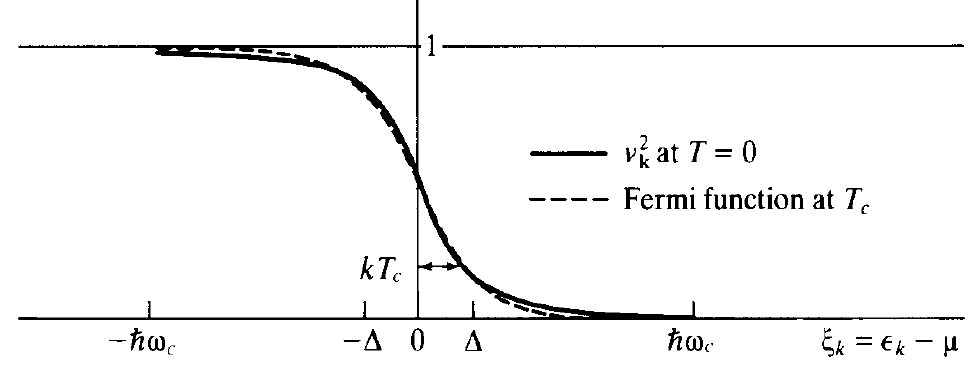
\includegraphics[width=0.8\textwidth]{immagini/andamento_nu_quadro.png}
\end{figure}
\hspace{-0.6cm}La parte sinistra dell'asse orizzontale corrisponde a valori negativi di $\xi(\vb{k})$, cioè energie inferiori al livello di Fermi, mentre la parte destra corrisponde a energie superiori.\\
Il comportamento di questo coefficiente fornisce informazioni importanti: nel sottospazio di Nambu associato a $\vb{k}$, $|\nu_{\vb{k}}|^2$ rappresenta la probabilità di trovare una coppia di elettroni (cioè una coppia di Cooper) con quella combinazione di momento e spin.\\
Analizziamo i regimi asintotici. Per $\varepsilon(\vb{k})<\mu$, cioè sotto il livello di Fermi, i livelli sono occupati nello stato normale, e infatti $|\nu_{\vb{k}}|^2 \to 1$. Per $\varepsilon(\vb{k})>\mu$, invece, i livelli sono vuoti e $|\nu_{\vb{k}}|^2 \to 0$.\\
Nella regione intermedia, dell'ordine di $\Delta$, la funzione presenta una transizione smussata, molto simile alla distribuzione di Fermi--Dirac a temperatura finita (indicata nel grafico con una linea tratteggiata).\\
È importante sottolineare che, nonostante la somiglianza, si tratta di quantità fisicamente diverse: da un lato abbiamo la probabilità di trovare una coppia di Cooper nello stato fondamentale BCS, dall'altro la probabilità di occupazione di uno stato a singola particella in un metallo normale a temperatura finita.\\
Questa somiglianza suggerisce però che gli stati elettronici rilevanti nello stato BCS sono quelli vicini al livello di Fermi, analogamente a quanto accade nel gas di Fermi a temperatura finita.\\
Questo è ragionevole, poiché la superconduttività emerge a una temperatura critica: gli elettroni che partecipano alla transizione sono proprio quelli vicini al livello di Fermi.\\
Tuttavia, esiste una differenza fondamentale: nello stato normale gli elettroni occupano stati indipendenti, senza coerenza di fase, mentre nello stato fondamentale BCS abbiamo una sovrapposizione coerente di stati a molti corpi. In questo caso non contano solo i moduli dei coefficienti, ma anche le loro fasi.\mn{Nel caso dello stato fondamentale BCS, a differenza del gas di Fermi normale, gli osservabili dipendono da combinazioni lineari dei coefficienti (come nel caso di $\expval*{\hat{\Delta}}$ che dipende da $u_{\vb{k}} \nu_{\vb{k}}^*$) e non solo dai loro moduli quadrati. Questo implica che le fasi relative dei coefficienti giocano un ruolo fisico fondamentale.}\\
In altre parole, lo stato fondamentale BCS è una sovrapposizione coerente di stati a molti corpi: una combinazione macroscopica con coerenza di fase. Questo è il senso in cui si dice che lo stato fondamentale BCS è uno stato coerente macroscopico.

\section{Lo stato coerente macroscopico}

Vediamo cosa significa affermare che lo stato fondamentale BCS è uno stato coerente macroscopico. Il termine macroscopico è intuitivo: deriva dal fatto che il sistema contiene un numero molto grande di particelle. Il termine coerente, invece, richiede qualche spiegazione.\\
Per prima cosa riscriviamo lo stato fondamentale BCS in una forma che permetta un confronto più immediato con uno stato coerente bosonico. Ricordiamo la sua espressione:
\begin{equation*}
   \ket{g_s}
   =\prod_{\vb{k}} \qty( u_{\vb{k}} \ket{0_{\vb{k}}} + \nu_{\vb{k}} \ket{2_{\vb{k}}} )
   =\prod_{\vb{k}} \qty( u_{\vb{k}} + \nu_{\vb{k}} Z^\dagger_{\vb{k}} ) \ket{0}
\end{equation*}
Possiamo riscriverlo come
\begin{equation*}
   \ket{g_s}
   =\prod_{\vb{k}} u_{\vb{k}} \qty( 1 + \frac{\nu_{\vb{k}}}{u_{\vb{k}}} Z^\dagger_{\vb{k}} ) \ket{0}
   = \text{cost.} \times \prod_{\vb{k}} \qty( 1 + \alpha_{\vb{k}} Z^\dagger_{\vb{k}} ) \ket{0}
\end{equation*}
dove abbiamo definito $\alpha_{\vb{k}}=\frac{\nu_{\vb{k}}}{u_{\vb{k}}}$ e la costante è data dal prodotto di tutti gli $u_{\vb{k}}$.\\
Ora cerchiamo di esprimere $u_{\vb{k}}$ e $\nu_{\vb{k}}$ in funzione di $\alpha_{\vb{k}}$. Dalla condizione di normalizzazione si ha
\begin{equation*}
   |u_{\vb{k}}|^2 + |\nu_{\vb{k}}|^2
   =|u_{\vb{k}}|^2 \qty( 1 + \frac{|\nu_{\vb{k}}|^2}{|u_{\vb{k}}|^2} )
   =|u_{\vb{k}}|^2 \qty( 1 + |\alpha_{\vb{k}}|^2 )
   =1
\end{equation*}
da cui segue
\begin{equation*}
   |u_{\vb{k}}|^2
   =\frac{1}{ 1 + |\alpha_{\vb{k}}|^2 }
   \qq{;}
   |\nu_{\vb{k}}|^2
   =\frac{ |\alpha_{\vb{k}}|^2 }{ 1 + |\alpha_{\vb{k}}|^2 }
\end{equation*}
Inoltre, l'operatore $\bigl( 1 + \alpha_{\vb{k}} Z^\dagger_{\vb{k}} \bigr)$ può essere riscritto come un esponenziale:\mn{Si presti attenzione al fatto che questa uguaglianza non vale in generale, ma perché $Z^\dagger_{\vb{k}}$ è costruito a partire da operatori fermionici, dunque soddisfa la relazione
\begin{equation*}
   \bigl(Z^\dagger_{\vb{k}}\bigr)^2 = 0
\end{equation*}
Di conseguenza, lo sviluppo in serie dell'esponenziale
\begin{equation*}
   e^{\alpha_{\vb{k}} Z^\dagger_{\vb{k}}}
   =\sum_{n=0}^{\infty} \frac{ (\alpha_{\vb{k}} Z^\dagger_{\vb{k}})^n }{n!}
\end{equation*}
si tronca automaticamente al primo ordine.}
\begin{equation*}
   1 + \alpha^{\vphantom{\dag}}_{\vb{k}} Z^\dagger_{\vb{k}}
   =e^{\alpha^{\vphantom{\dag}}_{\vb{k}} Z^\dagger_{\vb{k}}}
\end{equation*}
dunque lo stato fondamentale può essere riscritto come
\begin{equation}
   \ket{g_s}
   =\text{cost.} \times \prod_{\vb{k}} e^{\alpha_{\vb{k}} Z^\dagger_{\vb{k}}} \ket{0}
   =\text{cost.} \times \exp \Bigl( \sum_{\vb{k}} \alpha^{\vphantom{\dag}}_{\vb{k}} Z^\dagger_{\vb{k}} \Bigr) \ket{0}
   \label{eq:BCS_ground_state_forma_stato_coerente}
\end{equation}
A questo punto scriviamo l'espressione di uno stato coerente bosonico.\\
Uno stato coerente bosonico è uno stato $\ket*{\alpha}$ definito come
\begin{equation*}
   \ket*{\alpha}
   =\text{cost.} \times e^{\alpha a^{\dag}} \ket{0}
\end{equation*}
Questa espressione ha una forma molto simile a quella dello stato BCS, poiché $a^{\dag}$ è l'operatore di creazione bosonico. Tuttavia, bisogna prestare attenzione: si tratta di quantità diverse, a causa delle differenti statistiche. Infatti, $a^{\dag}$ è un operatore bosonico, mentre $Z^{\dag}_{\vb{k}}$ è un operatore composto da due operatori fermionici, e quindi non valgono le regole di commutazione bosoniche.\\
Nonostante ciò, possiamo osservare che i due stati hanno una struttura matematica molto simile.\\
L'obiettivo ora è capire perché questa analogia sia rilevante: non si tratta soltanto di una somiglianza formale, ma del fatto che alcune proprietà degli stati coerenti bosonici possono essere utilizzate per comprendere proprietà analoghe dello stato fondamentale BCS.
\subsection{Stati coerenti}
Facciamo adesso un breve ripasso sugli stati bosonici coerenti. Per tale scopo, consideriamo l'oscillatore armonico quantistico. L'operatore hamiltoniano di tale sistema è dato da
\begin{equation*}
   \hat{H} = \frac{\hat{p}^2}{2m} + \frac{m\omega^2}{2} \hat{x}^2
\end{equation*}
Gli autostati dell'oscillatore sono dati da
\begin{equation}
   \hat{H} \ket*{n} = E_n \ket*{n}
\end{equation}
dove $E_n$ sono i livelli energetici.\\
Il metodo più elegante per risolvere questo problema , ovvero per determinare energie ed autostati, consiste nell'introdurre gli operatori di creazione e distruzione, $a^{\dag}$ e $a$, mediante i quali possiamo esprimere gli operatori di posizione e momento come
\begin{equation*}
   \hat{x}=\text{cost.} \times (a + a^{\dag})
   \qq{;}
   \hat{p}=\text{cost.} \times (a^{\dag} - a)
\end{equation*}
con le costanti scelte in modo opportuno.\\
Tali operatori sono degli operatori bosonici e possiedono una serie di proprietà molto utili. Innanzitutto per essi vale la relazione di commutazione
\begin{equation}
   [a^{\dag}, a] = 1
   \label{eq:bosonic_commutation_relation}
\end{equation}
Inoltre, l'azione dell'operatore di creazione $a^{\dag}$ su uno stato di Fock, cioè uno stato con $n$ bosoni, è data da
\begin{equation*}
   a^{\dag} \ket{n} = \sqrt{n+1} \ket{n+1}
\end{equation*}
mentre l'azione dell'operatore di annichilazione è
\begin{equation*}
   a \ket{n} = \sqrt{n} \ket{n-1}
\end{equation*}
Possiamo definire l'operatore numero $\hat{n} = a^{\dag} a$, la cui azione su uno stato di Fock è
\begin{equation*}
   \hat{n} \ket{n} = n \ket{n}
\end{equation*}
In termini di questi operatori, l'Hamiltoniana dell'oscillatore è data da
\begin{equation*}
   \hat{H} = \hbar \omega \left( a^{\dag} a + \frac{1}{2} \right)
\end{equation*}
e in tale forma si ottiene immediatamente che i livelli energetici sono
\begin{equation*}
   E_n = \hbar \omega \left( n + \frac{1}{2} \right)
\end{equation*}
Per come agisce l'operatore di creazione $a^{\dag}$ su uno stato di Fock, è possibile costruire tutti gli autostati $\ket*{n}$ in modo iterativo, agendo ripetutamente sullo stato fondamentale iniziale $\ket{0}$:
\begin{equation}
   \ket*{n}=\frac{1}{\sqrt{n!}} {(a^{\dag})}^n \ket{0}
   \label{eq:formula_ricorsiva_autostati_oscillatore}
\end{equation}
Tali operatori hanno anche molti altri utilizzi. In particolare, definiamo uno stato coerente come
\begin{equation}
   \ket{\alpha} 
   = C \qty(
   \ket*{0}
   + \frac{\alpha}{\sqrt{1!}} \ket*{1}
   + \frac{\alpha^2}{\sqrt{2!}} \ket*{2}
   + \ldots )
   \label{eq:coherent_state}
\end{equation}
dove $\alpha$ è un numero complesso arbitrario e $C$ è una costante di normalizzazione. Quest'ultima può essere determinata dalla condizione di normalizzazione
\begin{equation*}
   1 = \braket*{\alpha}
   = |C|^2 \left( 1 + \frac{|\alpha|^2}{1!} + \frac{{(|\alpha|^2)}^2}{2!} + \ldots \right)
   = |C|^2 e^{|\alpha|^2}
\end{equation*}
da cui si ottiene
\begin{equation*}
   C = e^{-|\alpha|^2/2}
\end{equation*}
Gli stati coerenti possiedono molte proprietà interessanti. Notiamo innanzitutto che l'\eqrefcustom{eq:coherent_state} può essere riscritta in termini dell'operatore di creazione $a^{\dag}$. Utilizzando l'\eqrefcustom{eq:formula_ricorsiva_autostati_oscillatore} per ciascun termine si ha
\begin{equation*}
   \ket*{\alpha}
   = e^{-|\alpha|^2/2} \left( 1 + \frac{\alpha a^{\dag}}{1!} + \frac{(\alpha a^{\dag})^2}{2!} + \ldots \right) \ket*{0}
\end{equation*}
dove $\ket*{0}$ è lo stato fondamentale ed è anche lo stato coerente con $\alpha = 0$. Questa espressione può essere scritta in forma molto compatta come
\begin{equation*}
\ket*{\alpha} = e^{-|\alpha|^2/2} e^{\alpha a^{\dag}} \ket*{0}
\end{equation*}
dove abbiamo usato la definizione dell'esponenziale di un operatore $\hat{X}$ tramite lo sviluppo in serie
\begin{equation*}
   e^{\hat{X}} = 1 + \frac{\hat{X}}{1!} + \frac{\hat{X}^2}{2!} + \ldots
\end{equation*}
Un'altra relazione interessante, che può essere ottenuta dall'\eqrefcustom{eq:coherent_state}, è
\begin{equation}
   a \ket*{\alpha} = \alpha \ket*{\alpha}
   \label{eq:coherent_state_eigenvalue_equation}
\end{equation}
ovvero gli stati coerenti sono autostati dell'operatore di annichilazione $a$. Per dimostrarlo possiamo scrivere esplicitamente lo stato $a\ket*{\alpha}$:
\begin{equation*}
   a\ket*{\alpha}
   = e^{-|\alpha|^2/2} \, a
   \qty( \ket*{0} + \frac{\alpha}{\sqrt{1!}} \ket*{1} + \frac{\alpha^2}{\sqrt{2!}} \ket*{2} + \ldots )
\end{equation*}
Ma poiché $a\ket*{n} = \sqrt{n}\ket*{n-1}$, si ottiene
\begin{equation*}
   a\ket*{\alpha} = e^{-|\alpha|^2/2} \left( 0 + \frac{\alpha \sqrt{1}}{\sqrt{1!}} \ket*{0} + \frac{\alpha^2 \sqrt{2}}{\sqrt{2!}} \ket*{1} + \ldots \right)
\end{equation*}
che è chiaramente uguale a $\alpha \ket*{\alpha}$.\\
Infine, dall'\eqrefcustom{eq:coherent_state_eigenvalue_equation} segue che
\begin{equation*}
   \mel*{\alpha}{a^{\dag} a}{\alpha}
   =\bigl( \bra*{\alpha} a^{\dag} \bigr) \bigl( a \ket*{\alpha} \bigr)
   =\alpha^* \alpha \braket*{\alpha}
   = |\alpha|^2
\end{equation*}
Pertanto, il valore di $|\alpha|^2$ fornisce il valore medio dell'operatore numero $\expval*{\hat{n}}$ dello stato quantistico.\\
Estendendo questo risultato a $\hat{n}^2$ possiamo determinare l'incertezza sul numero $\Delta n$. Calcoliamo quindi $\expval*{\hat{n}^2}$:
\begin{equation*}
   \expval*{\hat{n}^2} = \mel*{\alpha}{a^{\dag} a a^{\dag} a}{\alpha}
\end{equation*}
dall'\eqrefcustom{eq:bosonic_commutation_relation} si ha che
\begin{equation*}
   [a^{\dag}, a] = a^{\dag} a - a a^{\dag} = 1
   \implies
   a a^{\dag} = a^{\dag} a + 1
\end{equation*}
Inserendo tale risultato precedenti, si ottiene
\begin{equation*}
   \expval*{\hat{n}^2}
   =\mel*{\alpha}{a^{\dag}(a^{\dag} a + 1) a }{\alpha}
   =\mel*{\alpha}{a^{\dag}a^{\dag} a a }{\alpha}
   + \mel*{\alpha}{a^{\dag} a}{\alpha}
\end{equation*}
Il secondo termine non è altro che $\expval*{\hat{n}}$, che abbiamo già calcolato essere $|\alpha|^2$. Per quanto riguarda il primo termine, possiamo riscriverlo come
\begin{equation*}
   \mel*{\alpha}{a^{\dag}a^{\dag} a a }{\alpha}
   =\bigl( \bra*{\alpha} a^{\dag}a^{\dag} \bigr) \bigl( a a \ket*{\alpha} \bigr)
\end{equation*}
Dato che vale l'\eqrefcustom{eq:coherent_state_eigenvalue_equation}, si ha che $a a \ket*{\alpha} = \alpha^2 \ket*{\alpha}$, e in maniera analoga $\bra*{\alpha} a^{\dag}a^{\dag} = {(\alpha^*)}^2 \bra*{\alpha}$, quindi
\begin{equation*}
   \mel*{\alpha}{a^{\dag}a^{\dag} a a }{\alpha}
   =|\alpha|^4
\end{equation*}
In definitiva abbiamo trovato che
\begin{equation*}
   \expval*{\hat{n}^2} = |\alpha|^4 + |\alpha|^2
\end{equation*}
Una volta calcolati $\expval*{\hat{n}}$ e $\expval*{\hat{n}^2}$, possiamo calcolare l'incertezza $\Delta n$:
\begin{equation*}
   \Delta n
   = \sqrt{\expval*{\hat{n}^2} - \expval*{\hat{n}}^2}
   = |\alpha|
\end{equation*}
Ora vogliamo determinare quale sia la relazione tra il numero medio di bosoni nello stato coerente e la sua varianza, in modo da poter valutare quale sia l'incertezza sul numero di bosoni nello stato coerente. Si ha che
\begin{equation}
   \frac{\Delta n}{\expval*{\hat{n}}}
   =\frac{|\alpha|}{|\alpha|^2}
   =\frac{1}{|\alpha|}
\end{equation}
Saremo principalmente interessati a stati coerenti macroscopici, per i quali $\expval*{\hat{n}}$, e quindi $|\alpha|$, è molto grande. Per tali stati, si può vedere che la deviazione standard $\Delta n$ diventa trascurabile rispetto a $\expval*{\hat{n}}$. Pertanto, come buona approssimazione, possiamo approssimare molti valori medi di operatori con i loro valori di campo medio ottenuti dalla sostituzione $\hat{n} \approx \expval*{\hat{n}}$.\\
Questo è, in un certo senso, qualcosa di simile a quanto abbiamo già visto per lo stato fondamentale BCS, che presenta una struttura in cui il numero medio di elettroni è molto grande, ma l'incertezza relativa è molto piccola. In questo senso esiste un'analogia, che deriva anche dalla struttura degli stati.\\
È importante notare che lo stato coerente $\ket*{\alpha}$ possiede una fase $\vartheta$ ben definita, pur non avendo un numero quantico $n$ definito. Infatti, il numero complesso $\alpha$ che descrive lo stato coerente può essere espresso come
\begin{equation*}
   \alpha = |\alpha| e^{i\vartheta}
\end{equation*}
e esprimendolo in tale forma all'interno dell'\eqrefcustom{eq:coherent_state} si ottiene
\begin{equation}
   \ket*{\alpha}
   = e^{-|\alpha|^2/2} 
   \qty( \ket*{0} + \frac{|\alpha| e^{i\vartheta}}{\sqrt{1!}} \ket*{1} + \frac{|\alpha|^2 e^{i2\vartheta}}{\sqrt{2!}} \ket*{2} + \ldots )
   \label{eq:coherent_state_polar_form}
\end{equation}
Si vede che il termine contenente $\ket*{n}$ dipende da $e^{in\vartheta}$. Ciò non ci sorprende in quanto, come abbiamo visto, gli stati coerenti sono sovrapposizioni di stati di Fock con numeri quantici $n$ diversi, e ciascuno di questi stati di Fock contribuisce con una fase.\\
Derivando l'\eqrefcustom{eq:coherent_state_polar_form} rispetto a $\vartheta$ si ottiene
\begin{equation*}
   \pdv{}{\vartheta} \ket*{\alpha}
   = e^{-|\alpha|^2/2} \qty( 0 + \frac{i |\alpha| e^{i\vartheta}}{\sqrt{1!}} \ket*{1} + \frac{2i |\alpha|^2 e^{i2\vartheta}}{\sqrt{2!}} \ket*{2} + \ldots )
\end{equation*}
Da cui si ricava
\begin{equation*}
   \frac{1}{i}\frac{\partial}{\partial \vartheta} \ket*{\alpha} = \hat{n} \ket*{\alpha}
\end{equation*}
Poiché gli stati $\ket*{\alpha}$ costituiscono un insieme completo (in realtà sovracompleto), possiamo effettuare l'identificazione tra operatori
\begin{equation*}
   \frac{1}{i}\frac{\partial}{\partial \vartheta} = \hat{n}
\end{equation*}
Pertanto, la fase $\vartheta$ e il numero $n$ sono operatori coniugati, in modo analogo a quanto accade per quantità di moto e posizione nella meccanica quantistica standard. Di conseguenza, è possibile formulare una relazione di indeterminazione per questi operatori:
\begin{equation*}
   \Delta n \, \Delta \vartheta \geq \frac{1}{2}
\end{equation*}
Gli stati coerenti hanno una fase ben definita, ma non possiedono un valore definito del numero quantico $n$. Al contrario, gli autostati di energia $\ket*{n}$ hanno un valore ben definito di $n$, ma una fase arbitraria (o indefinita).
\section{Proprietà dello stato fondamentale BCS}
\subsection{Rottura della simmetria di gauge}
Vediamo quali sono le implicazioni per lo stato fondamentale BCS.\\
La nostra osservazione iniziale è stata che lo stato fondamentale può essere scritto nella forma dell'\eqrefcustom{eq:BCS_ground_state_forma_stato_coerente}, che ha la stessa struttura di uno stato coerente bosonico. In questo senso, si tratta di uno stato coerente, ma di coppie di Cooper, poiché l'operatore $\hat{Z}^{\dag}$ crea coppie di Cooper.\\
Inoltre, in analogia con uno stato coerente bosonico, che possiede un valore definito di $\alpha$, anche lo stato coerente fermionico, almeno in ciascun sottospazio di Nambu per ogni $\vb{k}$, possiede una fase ben definita. Questa fase definita, analogamente al caso bosonico, implica un'incertezza nel numero di particelle, che in questo caso sono fermioni.\\
Il passo che stiamo compiendo ora consiste nel prendere l'analogia tra numero di particelle e fase che vale per gli stati coerenti e applicarla allo stato BCS.\\
Fissare $\alpha_{\vb{k}}$ significa fissare la fase relativa tra $\nu_{\vb{k}}$ e $u_{\vb{k}}$, cioè tra le componenti con zero e due elettroni. Tuttavia, una variazione di questa fase non modifica $|\Delta|$, che entra nel valore medio dell'energia nello stato BCS.\\
Questo significa che cambiando la fase di $\alpha_{\vb{k}}$ otteniamo stati con fasi diverse, ma energeticamente degeneri. Tuttavia, quando avviene la transizione e il sistema è descritto dallo stato fondamentale BCS, esso seleziona uno specifico valore di $\alpha_{\vb{k}}$, cioè coefficienti ben determinati. In altre parole, il sistema sceglie un valore specifico della fase.\\
Abbiamo quindi una famiglia di stati, tutti degeneri, corrispondenti a diversi valori di $\alpha_{\vb{k}}$, ma il sistema ne seleziona uno solo. Questo è precisamente ciò che si intende per rottura spontanea di simmetria, e la simmetria che viene rotta in questo caso è una simmetria di gauge.\\
Per riassumere, stiamo collegando le proprietà dello stato fondamentale BCS alla rottura della simmetria di gauge nella transizione superconduttiva. Abbiamo già introdotto questo concetto dal punto di vista della teoria di Ginzburg-Landau, ma qui lo vediamo emergere direttamente dalla struttura dello stato fondamentale BCS.\\
La struttura dello stato fondamentale BCS, espressa come stato coerente fermionico, è
\begin{equation*}
   \ket{g_s}
   =\text{cost.} \times \exp \Bigl( \sum_{\vb{k}} \alpha_{\vb{k}} Z^\dagger_{\vb{k}} \Bigr) \ket{0}
\end{equation*}
dove $\hat{Z}^{\dag}_{\vb{k}}$ è l'operatore che crea una coppia di elettroni con struttura di coppia di Cooper.\\
Inoltre, abbiamo derivato la forma dei coefficienti $u_{\vb{k}}$ e $\nu_{\vb{k}}$ e, in particolare, dobbiamo ricordare che il loro prodotto è semplicemente legato a $\Delta$, che è il valore medio dell'operatore $\hat{Z}_{\vb{k}}$, tramite l'\eqrefcustom{eq:BCS_u_nu_Delta_relation}.\\
Abbiamo anche visto che il valore medio dell'hamiltoniana BCS, meno il contributo introdotto per tenere conto del fatto che il numero di particelle non è fissato, valutato sullo stato fondamentale, è dato dall'\eqrefcustom{eq:BCS_energy}:
\begin{equation*}
   \mel*{g_s}{H - \mu N}{g_s}=\sum_{\vb{k}} 2 \xi(\vb{k}) |\nu_{\vb{k}}|^2 + V \Bigl| \sum_{\vb{k}} u_{\vb{k}} \nu^*_{\vb{k}} \Bigr|^2
\end{equation*}
Per quanto riguarda il primo termine, definendo
\begin{equation*}
   E_{\vb{k}}=\sqrt{\xi^2_{\vb{k}} + |\Delta|^2}
\end{equation*}
e inserendo l'\eqrefcustom{eq:coefficiente_nu_BCS} si ottiene
\begin{equation*}
   2 \sum_{\vb{k}} \xi_{\vb{k}} |\nu_{\vb{k}}|^2
   = 2 \sum_{\vb{k}} \xi_{\vb{k}} \frac{1}{2} \qty( 1 - \frac{\xi_{\vb{k}}}{E_{\vb{k}}} )
   = \sum_{\vb{k}} \qty( \xi_{\vb{k}} - \frac{\xi^2_{\vb{k}}}{E_{\vb{k}}} )
\end{equation*}
Per il secondo termine, invece, dalle definizioni di $\Delta$ e $\Delta^*$ segue che
\begin{equation*}
   V \Bigl| \sum_{\vb{k}} u_{\vb{k}} \nu^*_{\vb{k}} \Bigr|^2
   =\frac{|\Delta|^2}{V}
   =-\frac{|\Delta|^2}{|V|}
\end{equation*}
In definitiva
\begin{equation}
   \mel*{g_s}{H - \mu N}{g_s}
   = \sum_{\vb{k}} \qty( \xi_{\vb{k}} - \frac{\xi^2_{\vb{k}}}{E_{\vb{k}}} ) - \frac{|\Delta|^2}{|V|}
   \label{eq:BCS_energy_final_expression}
\end{equation}
Si noti che la somma è estesa a tutti i valori di $\vb{k}$ e non solo a quelli sopra o sotto il momento di Fermi.\\
A partire da qui, facciamo alcune osservazioni e colleghiamo queste proprietà alla rottura della simmetria di gauge. Innanzitutto, $\Delta$ è in generale una quantità complessa, quindi possiamo scrivere
\begin{equation*}
   \Delta = |\Delta| e^{i\phi}
\end{equation*}
Osserviamo che l'energia è reale e dipende solo da $|\Delta|^2$, mentre i coefficienti $u_{\vb{k}}$ e $\nu_{\vb{k}}$, che possono essere complessi, dipendono da $\Delta$. Ciò implica che, variando la fase di $\Delta$, si ottengono coefficienti $u_{\vb{k}}$ e $\nu_{\vb{k}}$ diversi. In particolare, tutti i coefficienti cambiano fase nello stesso modo, cioè questa fase non dipende da $\vb{k}$. Di conseguenza, la fase relativa tra i coefficienti che definiscono le coppie di Cooper è la stessa per tutti gli stati.\\
Questo significa che valori diversi del parametro complesso $\Delta$ corrispondono a stati diversi, poiché cambiano i coefficienti della sovrapposizione che definisce lo stato fondamentale, ma tutti questi stati hanno la stessa energia. Quindi tutti gli stati che differiscono per una fase globale, comune a tutti i $\vb{k}$, sono degeneri. Ciò porta naturalmente alla rottura di una simmetria: se il sistema si trova in uno stato fondamentale con una fase specifica, pur esistendo infiniti stati degeneri con la stessa energia, significa che è stata effettuata una scelta tra stati equivalenti. Questo è analogo a quanto accade nella transizione ferromagnetica, dove il sistema sceglie una direzione di magnetizzazione tra infinite direzioni energeticamente equivalenti.\\
Tale fatto è quindi un chiaro segnale dell'avvenire di una transizione. Il tipo di simmetria che viene rotta, come già anticipato, è la simmetria di gauge.\\
Richiamiamo brevemente quale tipo di simmetria di gauge abbiamo considerato. Per una singola particella, possiamo avere una trasformazione di gauge globale o locale. Una trasformazione globale consiste nel moltiplicare la funzione d'onda $\psi$ per una fase costante:
\begin{equation*}
   \psi \rightarrow e^{i\chi} \psi
\end{equation*}
Questi stati sono fisicamente equivalenti, riflettendo l'ambiguità di fase intrinseca della meccanica quantistica.\\
Possiamo anche considerare una trasformazione di gauge locale, in cui la fase dipende da spazio e tempo:
\begin{equation*}
   \psi(\vb{r},t)
   \longrightarrow
   \psi(\vb{r},t) e^{i \frac{q \chi(\vb{r},t)}{\hbar}}
   \equiv \tilde{\psi}(\vb{r},t)
\end{equation*}
Se $\psi$ soddisfa l'equazione di Schrödinger
\begin{equation*}
   i \hbar \pdv{\psi}{t}
   =-\frac{\hbar^2}{2m} \laplacian{\psi}
\end{equation*}
allora $\tilde{\psi}$ soddisfa l'equazione modificata
\begin{equation*}
   i \hbar \pdv{\tilde{\psi}}{t}
   =\qty[ -\frac{\hbar^2}{2m} \qty( \grad - i \frac{q}{\hbar} \vb{A} )^2 + q\Phi ] \tilde{\psi}
   \qq{dove}
   \begin{dcases}
   \Phi = -\pdv{\chi}{t}
   \\
   \vb{A} = \grad \chi
   \end{dcases}
\end{equation*}
Consideriamo ora un sistema a molte particelle, in particolare lo stato fondamentale BCS. Partiamo dallo stato di Fock $\ket*{\{ n_{\vb{k}} \} }$, dove $n_k$ è il numero di occupazione del livello $k$, che per i fermioni può essere 0 o 1. Se applichiamo una trasformazione di fase globale a ciascuna particella, ogni stato $\ket*{n_k}$ diventa $e^{i\chi} \ket*{n_k}$, e lo stato complessivo acquista una fase globale:
\begin{equation*}
   \ket*{\{ n_{\vb{k}} \} }
   \longrightarrow
   e^{i N \chi} \ket*{\{ n_{\vb{k}} \} }
\end{equation*}
dove $N$ è il numero totale di elettroni.\\
Poiché $n_k$ sono autovalori dell'operatore numero $\hat{n}_k = c_k^\dagger c_k$, possiamo ottenere questo effetto modificando gli operatori di creazione:
\begin{equation*}
   c_k^\dagger \longrightarrow e^{i\chi} c_k^\dagger
\end{equation*}
Questa trasformazione non modifica l'operatore numero, poiché il fattore di fase si cancella con quello dell'hermitiano coniugato. In altre parole, le osservabili restano invarianti, come richiesto.
\subsection{Relazione di indeterminazione fase--numero}
Vediamo cosa accade allo stato fondamentale BCS se effettuiamo una trasformazione di fase globale su ciascuno degli elettroni che partecipano allo stato. Ricordiamo la forma dello stato, descritta dall'\eqrefcustom{eq:BCS_trial_wavefunction_Nambu}:
\begin{equation*}
   \ket{\psi_g}
   =\prod_{\vb{k}} \bigl( u_{\vb{k}} + \nu_{\vb{k}} \hat{Z}^{\dag}_{\vb{k}} \bigr) \ket*{\phi_0}
\end{equation*}
Ricordiamo inoltre che $\hat{Z}^{\dag}_{\vb{k}}$ è il prodotto di due operatori di creazione relativi a due elettroni con la corretta combinazione di momento e spin, cioè $c^{\dag}_{\vb{k},\uparrow} c^{\dag}_{-\vb{k},\downarrow}$. Se modifichiamo ciascun operatore di creazione introducendo il fattore di fase, allora l'operatore di creazione di coppia si trasforma nel modo seguente:
\begin{equation*}
   \hat{Z}^{\dag}_{\vb{k}}
   \longrightarrow
   e^{2i\chi} \hat{Z}^{\dag}_{\vb{k}}
\end{equation*}
Ciò implica che lo stato fondamentale BCS si trasforma in
\begin{equation*}
   \ket{\psi_g}
   \longrightarrow
   \ket*{\psi_{\chi}}
   =
   \prod_{\vb{k}=\vb{k}_1,\ldots,\vb{k}_M}
   \bigl(
      u_{\vb{k}}
      +
      \nu_{\vb{k}} e^{2i\chi}
      c^{\dag}_{\vb{k},\uparrow}
      c^{\dag}_{-\vb{k},\downarrow}
   \bigr)\ket*{0}
\end{equation*}
Se osserviamo questo stato senza preoccuparci momentaneamente della sua origine, possiamo interpretare questa trasformazione come una modifica della fase relativa tra $u_{\vb{k}}$ e $\nu_{\vb{k}}$, ed è proprio questo il punto che avevamo anticipato in precedenza: stiamo modificando la fase relativa tra questi coefficienti senza alterare l'energia dello stato. Ciò significa che lo stato $\ket*{\psi_{\chi}}$ appartiene alla famiglia di stati degeneri di cui abbiamo parlato in precedenza. In altre parole, i diversi stati fondamentali aventi la stessa energia ma differente fase possono essere scritti in questa forma. Quando il sistema seleziona uno stato particolare, esso sceglie una fase definita. Questo corrisponde alla rottura della simmetria di gauge, poiché si tratta esattamente dello stesso tipo di trasformazione di gauge globale discusso in precedenza.\\
Avere una fase definita corrisponde però a non avere un numero di particelle ben definito. Compare infatti una relazione di indeterminazione tra fase e numero di particelle, analoga a quella tra posizione e quantità di moto. Questo può essere visto facilmente partendo da uno stato generico $\ket*{\psi_{\chi}}$. Poiché sappiamo che si tratta di uno stato a molte particelle, possiamo scriverlo come sovrapposizione di stati a numero fissato di particelle:
\begin{equation*}
   \ket*{\psi_{\chi}}
   =
   \sum_N
   \lambda_N e^{i N \chi}
   \ket*{\psi_N}
\end{equation*}
I coefficienti $\lambda_N$ sono incogniti e, in linea di principio, possono essere determinati a partire dalla forma esplicita dello stato fondamentale BCS. Inoltre, sappiamo che ciascuno stato $\ket*{\psi_N}$ deve acquisire una fase del tipo $e^{i N \chi}$, proprio perché deriva dalla trasformazione dello stato BCS. Questa scrittura rappresenta quindi un modo formale di descrivere lo stato BCS come uno stato a molte particelle in cui le coppie possono essere occupate oppure no, ma mantenendo una relazione di fase ben definita tra le componenti con diverso numero di particelle, cioè una coerenza quantistica tra tali componenti.\\
Possiamo ora chiederci se sia possibile estrarre dallo stato fondamentale BCS la componente con numero fissato di particelle. In altre parole, dato uno stato generale della forma
\begin{equation*}
   \ket*{\psi}
   =
   \sum_i a_i \ket*{\psi_i}
\end{equation*}
possiamo domandarci se sia possibile determinare il peso $|a_i|^2$ dei vari stati oppure verificare se un certo stato $\ket*{\psi_j}$ appartenga alla sovrapposizione.\\
Normalmente, ciò che si fa è proiettare lo stato sul vettore desiderato. Se $\ket*{\psi_j}$ appartiene alla base dello spazio di Hilbert, allora:
\begin{equation*}
   \braket*{\psi_j}{\psi}
   =\sum_i a_i \braket*{\psi_j}{\psi_i}
   =a_j
\end{equation*}
Nel caso dello stato fondamentale BCS, possiamo sfruttare la decomposizione in stati a numero fissato di particelle e moltiplicare $\ket*{\psi_{\chi}}$ per una fase $e^{-i \bar{N} \chi}$:
\begin{equation*}
   e^{-i \bar{N} \chi}
   \ket*{\psi_{\chi}}
   =
   \sum_N
   \lambda_N
   e^{i\chi (N-\bar{N})}
   \ket*{\psi_N}
\end{equation*}
Poiché $\chi$ è un parametro libero, possiamo integrare tale espressione rispetto ad esso:
\begin{equation*}
   \int_0^{2\pi}
   \dd{\chi}\,
   e^{-i \bar{N} \chi}
   \ket*{\psi_{\chi}}
   =
   \sum_N
   \lambda_N
   \ket*{\psi_N}
   \int_0^{2\pi}
   \dd{\chi}\,
   e^{i\chi(N-\bar{N})}
\end{equation*}
Ma l'integrale della funzione esponenziale è nullo per tutti i valori di $N$ diversi da $\bar{N}$,\mn{Ricordiamo infatti che
\begin{equation*}
   \int_0^{2\pi}
   \dd{x}\,
   e^{ix(\alpha-\alpha')}
   =
   2\pi \delta_{\alpha,\alpha'}
\end{equation*}
}
quindi otteniamo
\begin{equation*}
   \int_0^{2\pi}
   \dd{\chi}\,
   e^{-i \bar{N} \chi}
   \ket*{\psi_{\chi}}
   =
   2\pi \lambda_{\bar{N}}
   \ket*{\psi_{\bar{N}}}
\end{equation*}
L'integrale seleziona quindi esclusivamente la componente con numero di particelle pari a $\bar{N}$. Dal punto di vista matematico questo passaggio è piuttosto semplice, ma il suo significato fisico è molto importante. Se vogliamo estrarre dallo stato fondamentale BCS la componente a numero fissato di particelle, dobbiamo rendere completamente indeterminata la fase $\chi$ che caratterizza lo stato, poiché stiamo integrando su tutti i valori possibili di $\chi$ tra $0$ e $2\pi$. Questo mostra che lo stato fondamentale BCS è uno stato a fase definita ma con numero di particelle non definito. Si tratta quindi di una manifestazione della relazione di indeterminazione tra fase e numero di particelle, nella teoria BCS sono due variabili coniugate, e se vogliamo fissare una di esse, l'altra diventa completamente indeterminata.\\
Questa osservazione è importante perché ci si potrebbe chiedere quale sia il significato fisico di uno stato con numero di particelle non fissato. Una descrizione di questo tipo sarebbe infatti priva di senso per un sistema contenente poche particelle. Tuttavia, nel caso di un superconduttore macroscopico, il numero di particelle è enorme, e in questa situazione l'incertezza relativa sul numero di particelle diventa trascurabile. Le cose cambiano invece quando si considerano campioni sempre più piccoli, entrando nel regime mesoscopico o addirittura in sistemi ancora più piccoli. Più avanti nel corso vedremo infatti cosa accade quando il numero di particelle diminuisce progressivamente.\\
A questo punto sorge una domanda naturale: è possibile ``misurare'' la fase dello stato fondamentale superconduttivo? La risposta è sì, attraverso il fenomeno che discuteremo nel seguito, cioè l'effetto Josephson. Questo effetto si manifesta quando due superconduttori sono separati, nella situazione più semplice, da una sottile barriera isolante. L'effetto Josephson consiste nella presenza di una supercorrente che attraversa la barriera e che dipende dalla differenza tra le due fasi $\phi_1$ e $\phi_2$ dei superconduttori:
\begin{equation*}
   I \propto \sin(\phi_1-\phi_2)
\end{equation*}
La quantità osservabile è quindi una supercorrente che dipende direttamente dalle fasi associate agli stati macroscopici BCS dei due superconduttori.\\
Si tratta di un'affermazione molto forte, perché la supercorrente è una quantità macroscopicamente misurabile e dipende direttamente da proprietà macroscopiche dello stato fondamentale descritto dalla funzione d'onda BCS. In altre parole, un effetto quantistico collettivo dà origine a una quantità osservabile su scala macroscopica, e questo, dal punto di vista della meccanica quantistica, non è affatto banale.
\subsection{Energia di condensazione}
Vogliamo adesso derivare la cosiddetta energia di condensazione, ossia la differenza tra il valor medio dell'hamiltoniana BCS nello stato fondamentale superconduttivo e quello dell'hamiltoniana degli elettroni liberi. Questa quantità coincide con la differenza tra le energie del sistema nella fase superconduttiva e nella fase normale a temperatura nulla, cioè $U_s-U_n$, e rappresenta quindi il guadagno energetico associato alla formazione dello stato superconduttivo al di sotto della temperatura critica.\\
Dobbiamo quindi valutare la quantità
\begin{equation*}
   \mel*{g_s}{\hat{H} - \mu \hat{N}}{g_s}
   -
   \mel*{g_n}{\hat{H} - \mu \hat{N}}{g_n}
\end{equation*}
Abbiamo già trovato che il primo valor medio è dato dall'\eqrefcustom{eq:BCS_energy_final_expression}:
\begin{equation*}
   \mel*{g_s}{H - \mu N}{g_s}
   = \sum_{\vb{k}} \qty( \xi_{\vb{k}} - \frac{\xi^2_{\vb{k}}}{E_{\vb{k}}} ) - \frac{|\Delta|^2}{|V|}
\end{equation*}
mentre il secondo è il valor medio dello stesso operatore nello stato fondamentale normale del gas di Fermi. Sappiamo che nello stato fondamentale di un gas di Fermi normale tutti gli stati elettronici sono occupati fino al livello di Fermi; di conseguenza, l'energia misurata rispetto all'energia di Fermi (cioè rispetto al potenziale chimico) è semplicemente\mn{\cite{Tinkham} Come osservato in precedenza, lo stato normale a $T=0$ corrisponde allo stato BCS con $\Delta=0$, nel qual caso $E_{\vb{k}} = |\xi_{\vb{k}}|$.}
\begin{equation*}
   \mel*{g_n}{H - \mu N}{g_n}
   =\sum_{k < k_F} 2\xi_{\vb{k}}
\end{equation*}
Queste energie sono tutte negative perché gli stati si trovano al di sotto dell'energia di Fermi, quindi questa quantità risulta complessivamente negativa.\\
A questo punto dobbiamo scrivere esplicitamente la differenza tra queste due quantità. Per farlo, osserviamo che nell'\eqrefcustom{eq:BCS_energy_final_expression} la somma è estesa a tutti i valori di $\vb{k}$; possiamo quindi separarla nei contributi con $k<k_F$ e $k>k_F$. Otteniamo
\begin{equation*}
   \begin{split}
      \expval*{E}_s - \expval*{E}_n
      & =
      \sum_{k<k_F}
      \qty(
      \xi_{\vb{k}}
      -
      \frac{\xi^2_{\vb{k}}}{E_{\vb{k}}}
      )
      + \sum_{k > k_F} \qty( \xi_{\vb{k}} - \frac{\xi^2_{\vb{k}}}{E_{\vb{k}}} )
      - \frac{|\Delta|^2}{|V|}
      - \sum_{k < k_F} 2\xi_{\vb{k}}
      \\
      & =
      \sum_{k<k_F} \qty( -\xi_{\vb{k}} - \frac{\xi^2_{\vb{k}}}{E_{\vb{k}}} )
      -\frac{|\Delta|^2}{|V|}
      + \sum_{k > k_F} \qty( \xi_{\vb{k}} - \frac{\xi^2_{\vb{k}}}{E_{\vb{k}}} )
   \end{split}
\end{equation*}
Osserviamo che per $k<k_F$ si ha $\xi_{\vb{k}}<0$, quindi $-\xi_{\vb{k}}>0$. Questo rende la somma sui valori con $k<k_F$ simmetrica rispetto a quella sui valori con $k>k_F$, perché per questi ultimi si ha $\xi_{\vb{k}}>0$. Possiamo quindi sommare insieme i due contributi e ottenere
\begin{equation*}
   \mel*{g_s}{\hat{H} - \mu \hat{N}}{g_s}
   -
   \mel*{g_n}{\hat{H} - \mu \hat{N}}{g_n}
   =
   2 \sum_{k > k_F}
   \qty(
   \xi_{\vb{k}}
   -
   \frac{\xi^2_{\vb{k}}}{E_{\vb{k}}}
   )
   -
   \frac{|\Delta|^2}{|V|}
\end{equation*}
Il passo successivo consiste nel valutare tale somma. Per farlo passiamo al limite del continuo\mn{Da notare che, poiché la sommatoria è estesa solo per $k>k_F$, l'intervallo di energia sarà $[0,\hbar \omega_D]$, anziché $[-\hbar \omega_D, \hbar \omega_D]$.}:
\begin{equation*}
   \sum_{k > k_F} \qty( \xi_{\vb{k}} - \frac{\xi^2_{\vb{k}}}{E_{\vb{k}}} )
   =N(0) \int_{0}^{\hbar \omega_D} \dd{\xi} \qty( \xi - \frac{\xi^2}{\sqrt{\xi^2 + |\Delta|^2}} )
\end{equation*}
dove abbiamo assunto che la densità degli stati sia costante e pari al suo valore al livello di Fermi. Svolgendo l'integrale si ottiene
\begin{equation*}
   N(0)
   \qty{
      \frac{(\hbar \omega_D)^2}{2}
      -
      \qty[
         \frac{\hbar \omega_D}{2}
         \sqrt{
            (\hbar \omega_D)^2 + |\Delta|^2
         }
         -
         \frac{|\Delta|^2}{2}
         \operatorname{arcsinh}
         \qty(
            \frac{\hbar \omega_D}{|\Delta|}
         )
      ]
   }
\end{equation*}
A questo punto espandiamo i due termini presenti nella parentesi quadra assumendo $\hbar \omega_D \gg |\Delta|$. Per farlo riscriviamo l'espressione precedente come
\begin{equation*}
   N(0)
   \qty{
      \frac{(\hbar \omega_D)^2}{2}
      -
      \qty[
         \frac{(\hbar \omega_D)^2}{2}
         \sqrt{
            1
            +
            \frac{|\Delta|^2}{(\hbar \omega_D)^2}
         }
         -
         \frac{|\Delta|^2}{2}
         \operatorname{arcsinh}
         \qty(
            \frac{\hbar \omega_D}{|\Delta|}
         )
      ]
   }
\end{equation*}
Utilizziamo quindi l'approssimazione
\begin{equation*}
   \sqrt{1+x}\approx 1+\frac{x}{2}
   \qq{per} x\ll 1
\end{equation*}
e la condizione di autoconsistenza data dalla \eqrefcustom{eq:BCS_self_consistency_equation}. In questo modo possiamo scrivere
\begin{equation*}
   \begin{split}
      &
      N(0)
      \qty{
         \frac{(\hbar \omega_D)^2}{2}
         -
         \qty[
            \frac{(\hbar \omega_D)^2}{2}
            \qty(
               1
               +
               \frac{|\Delta|^2}{2(\hbar \omega_D)^2}
            )
            -
            \frac{|\Delta|^2}{2N(0)|V|}
         ]
      }
      \\[0.2cm]
      =\,&
      N(0)
      \qty{
         -\frac{|\Delta|^2}{4}
         +
         \frac{|\Delta|^2}{2N(0)|V|}
      }
      \\
      =\,&
      -\frac{N(0)|\Delta|^2}{4}
      +
      \frac{|\Delta|^2}{2|V|}
   \end{split}
\end{equation*}
In conclusione otteniamo
\begin{equation*}
   \sum_{k > k_F}
   \qty(
   \xi_{\vb{k}}
   -
   \frac{\xi^2_{\vb{k}}}{E_{\vb{k}}}
   )
   =
   -\frac{N(0)|\Delta|^2}{4}
   +
   \frac{|\Delta|^2}{2|V|}
\end{equation*}
Sostituendo questo risultato nell'energia di condensazione otteniamo
\begin{equation*}
   \expval*{E}_s - \expval*{E}_n
   =
   -\frac{N(0)|\Delta|^2}{2}
   +
   \frac{|\Delta|^2}{|V|}
   -
   \frac{|\Delta|^2}{|V|}
   =
   -\frac{N(0)|\Delta|^2}{2}
\end{equation*}
Come possiamo vedere, questa differenza è negativa. Ciò significa che lo stato fondamentale superconduttivo è più stabile dello stato normale. Inoltre, essa dipende direttamente dal parametro $\Delta$, che nasce essenzialmente dall'interazione attrattiva tra elettroni.\\
Questa quantità, ottenuta a partire da una descrizione quantomeccanica, non è altro che la differenza tra l'energia interna dello stato superconduttivo a temperatura nulla e quella dello stato normale alla stessa temperatura:
\begin{equation*}
   U_s(T=0)-U_n(T=0)=-\frac{N(0)|\Delta|^2}{2}
\end{equation*}
Questa differenza di energie libere a temperatura nulla, o più in generale al di sotto della temperatura critica, coincide con la definizione termodinamica del campo critico. Otteniamo quindi una relazione diretta tra una quantità macroscopica, il campo critico, e il parametro $\Delta$:
\begin{equation*}
   -\frac{N(0)|\Delta|^2}{2}
   =
   -\frac{H_c(0)^2}{8\pi}
\end{equation*}
Dall'\eqrefcustom{eq:BCS_gap_equation} sappiamo che $|\Delta| \propto \hbar \omega_D$, quindi questa relazione collega immediatamente il campo critico all'energia di Debye, che è una proprietà dei fononi del reticolo cristallino che costituisce il materiale superconduttore.\\
Questo è precisamente il modo in cui la teoria BCS spiega l'effetto isotopico, cioè la dipendenza del campo magnetico critico dalla massa isotopica degli atomi che formano il materiale superconduttore. Si trattava infatti di una delle osservazioni più sorprendenti agli inizi dello studio della superconduttività, perché non esisteva una spiegazione semplice che collegasse proprietà elettromagnetiche, come il campo critico che segnala la transizione, alle proprietà fononiche del metallo. Questo costituiva quindi una chiara indicazione del fatto che un qualche meccanismo fononico dovesse giocare un ruolo fondamentale nel fenomeno della superconduttività. Ora abbiamo derivato questa connessione direttamente dalla teoria BCS.
\section{Eccitazioni di un superconduttore}
Finora abbiamo discusso le proprietà a temperatura nulla. Ora invece passiamo alla natura delle eccitazioni e, a partire da esse, deriviamo le proprietà termodinamiche del superconduttore, cioè quelle che abbiamo introdotto all'inizio. Vedremo quindi come, a partire dalla teoria microscopica, sia possibile ottenere le forme esplicite della temperatura critica, del gap e della dipendenza del gap dalla temperatura, risultati che avevamo introdotto nella parte iniziale.\\
Il punto di partenza è l'Hamiltoniana di pairing, che abbiamo già introdotto diverse volte:
\begin{equation*}
   \hat{H} - \mu \hat{N}
   =
   \sum_{\vb{k},\sigma} \xi_{\vb{k}} \hat{n}_{\vb{k},\sigma}
   - V
   \Bigl( \sum_{\vb{k}} \hat{Z}^{\dag}_{\vb{k}} \Bigr)
   \Bigl( \sum_{\vb{k}} \hat{Z}_{\vb{k}} \Bigr)
   =
   \sum_{\vb{k},\sigma} \xi_{\vb{k}} \hat{n}_{\vb{k},\sigma}
   - \frac{1}{V} \hat{\Delta}^{\dag} \hat{\Delta}
\end{equation*}
L'idea per trovare le eccitazioni consiste nel considerare lo stato fondamentale BCS come stato di riferimento e valutare piccole eccitazioni (come l'aggiunta di una particella o di una lacuna) rispetto a tale stato. Procederemo trattando il problema nell'approssimazione di campo medio, che abbiamo già utilizzato per derivare la forma esplicita dell'energia BCS. Qui, tuttavia, applicheremo l'approssimazione di campo medio direttamente a livello dell'Hamiltoniana.\\
La procedura standard quando si hanno operatori fermionici si basa sul teorema di Wick, che permette di esprimere il valor medio di prodotti di operatori fermionici contenenti più di due operatori (come nel caso dei quattro operatori presenti nel termine di interazione) in termini di prodotti di operatori che coinvolgono solo due operatori fermionici, moltiplicati per il valor medio degli altri due.\\
Il teorema di Wick fornisce quindi una regola per scrivere il valor medio di quattro operatori fermionici includendo tutte le possibili permutazioni degli operatori fermionici e i corrispondenti valori medi dei termini rimanenti. In particolare, nel nostro caso i quattro operatori presenti nel termine di interazione sono $c^{\dag}_{\vb{k}',\uparrow} c^{\dag}_{-\vb{k}',\downarrow} c^{\vphantom{\dag}}_{-\vb{k},\downarrow} c^{\vphantom{\dag}}_{\vb{k},\uparrow}$, e l'approssimazione che effettuiamo sull'Hamiltoniana consiste nel sostituire questo prodotto con la combinazione seguente:
\begin{equation*}
   c^{\dag}_{\vb{k}',\uparrow}
   c^{\dag}_{-\vb{k}',\downarrow}
   c^{\vphantom{\dag}}_{-\vb{k},\downarrow}
   c^{\vphantom{\dag}}_{\vb{k},\uparrow}
   \approx
   \expval*{
      c^{\dag}_{\vb{k}',\uparrow}
      c^{\dag}_{-\vb{k}',\downarrow}
   }
   c^{\vphantom{\dag}}_{-\vb{k},\downarrow}
   c^{\vphantom{\dag}}_{\vb{k},\uparrow}
   +
   c^{\dag}_{\vb{k}',\uparrow}
   c^{\dag}_{-\vb{k}',\downarrow}
   \expval*{
      c^{\vphantom{\dag}}_{-\vb{k},\downarrow}
      c^{\vphantom{\dag}}_{\vb{k},\uparrow}
   }
\end{equation*}
Osserviamo che stiamo trascurando i valori medi di coppie di operatori nella forma creazione--annichilazione, come ad esempio $\expval*{
c^{\dag}_{\vb{k},\uparrow}
c^{\vphantom{\dag}}_{\vb{k},\uparrow}
}$. La ragione è che, per ciò che ci interessa, cioè partire dallo stato fondamentale BCS e considerare le eccitazioni a energia più bassa, queste combinazioni non differiscono sostanzialmente da quelle del gas di Fermi a temperatura nulla. Infatti tali operatori contano semplicemente se l'elettrone $(\vb{k},\uparrow)$ o quello $(-\vb{k},\downarrow)$ è presente oppure no, e sappiamo che a temperatura nulla tali stati sono occupati sia nel gas di Fermi normale sia nello stato fondamentale BCS, anche se con combinazioni differenti. Naturalmente lo stato complessivo è diverso, ma la probabilità di trovare il singolo elettrone è essenzialmente la stessa.\\
Il nostro punto di partenza è quindi l'Hamiltoniana di pairing nell'approssimazione di campo medio:
\begin{equation*}
   [H - \mu N]_{\rm MF}
   =
   \sum_{\vb{k},\sigma}
   \xi_{\vb{k}}
   n_{\vb{k},\sigma}
   -
   \Delta
   \sum_{\vb{k}}
   Z^{\dag}_{\vb{k}}
   -
   \Delta^*
   \sum_{\vb{k}}
   Z^{\vphantom{\dag}}_{\vb{k}}
   %+\frac{1}{V} |\Delta|^2
\end{equation*}
Abbiamo il termine degli elettroni liberi, in cui l'energia è sempre misurata rispetto al livello di Fermi, e poi termini che coinvolgono il valor medio di somme di operatori che creano o annichilano coppie di elettroni.\\
A questo punto ci si potrebbe chiedere rispetto a quale stato venga effettuato questo valor medio. Si tratta del valor medio sullo stato fondamentale BCS, ed è proprio per questo che lo consideriamo come stato di riferimento.\\
Il punto importante è che questa Hamiltoniana è quadratica, nel senso che coinvolge solo coppie di operatori fermionici, sia attraverso gli operatori numero sia negli altri termini. Inoltre, la struttura dell'Hamiltoniana è essenzialmente una somma sui diversi box di Nambu, cioè sui sottospazi in cui, in linea di principio, possiamo costruire i quattro stati possibili ottenuti considerando le due configurazioni elettroniche $(\vb{k},\uparrow)$ e $(-\vb{k},\downarrow)$ occupate oppure vuote. In particolare, finora abbiamo considerato solo il sottospazio bidimensionale generato dagli stati con zero oppure una coppia di Cooper; non abbiamo ancora incluso le eccitazioni, che entreranno invece in gioco adesso.\\
L'idea è quindi che questa Hamiltoniana possa essere scritta come somma sui diversi box di Nambu:
\begin{equation*}
   [\hat{H} - \mu \hat{N}]_{\rm MF}
   = \sum_{\vb{k}} \hat{H}_{\vb{k}}
\end{equation*}
e in ciascun box di Nambu abbiamo un'Hamiltoniana dalla struttura molto semplice:
\begin{equation*}
   \hat{H}_{\vb{k}}
   =
   \sum_{\sigma}
   \xi_{\vb{k}}
   \hat{n}_{\vb{k},\sigma}
   -
   \Delta
   \hat{Z}^{\dag}_{\vb{k}}
   -
   \Delta^*
   \hat{Z}^{\vphantom{\dag}}_{\vb{k}}
   %+\frac{1}{V} |\Delta|^2
\end{equation*}
Questa espressione può essere riscritta in forma matriciale:
\begin{equation*}
   \hat{H}_{\vb{k}}
   =
   \begin{pmatrix}
      c^{\dag}_{\vb{k},\uparrow}
      &
      c^{\vphantom{\dag}}_{-\vb{k},\downarrow}
   \end{pmatrix}
   \begin{pmatrix}
      \xi_{\vb{k}} & -\Delta\\[0.2cm]
      -\Delta^* & -\xi_{\vb{k}}
   \end{pmatrix}
   \begin{pmatrix}
      c^{\vphantom{\dag}}_{\vb{k},\uparrow}\\[0.2cm]
      c^{\dag}_{-\vb{k},\downarrow}
   \end{pmatrix}
   - \xi_{\vb{k}}
\end{equation*}
Vediamo esplicitamente come ottenere questa forma. Scriviamo tutti i termini tramite operatori di creazione e annichilazione:
\begin{equation*}
   \hat{H}_{\vb{k}}
   =
   \xi_{\vb{k}}
   \bigl(
      c^{\dag}_{\vb{k}, \uparrow}
      c^{\vphantom{\dag}}_{\vb{k}, \uparrow}
      +
      c^{\dag}_{-\vb{k}, \downarrow}
      c^{\vphantom{\dag}}_{-\vb{k}, \downarrow}
   \bigr)
   -
   \Delta
   c^{\dag}_{\vb{k}, \uparrow}
   c^{\dag}_{-\vb{k}, \downarrow}
   -
   \Delta^*
   c^{\vphantom{\dag}}_{-\vb{k}, \downarrow}
   c^{\vphantom{\dag}}_{\vb{k}, \uparrow}
\end{equation*}
Usando le relazioni di anticommutazione degli operatori fermionici possiamo scrivere
\begin{equation*}
   c^{\dag}_{-\vb{k}, \downarrow}
   c^{\vphantom{\dag}}_{-\vb{k}, \downarrow}
   =
   1
   -
   c^{\vphantom{\dag}}_{-\vb{k}, \downarrow}
   c^{\dag}_{-\vb{k}, \downarrow}
\end{equation*}
ed è proprio per questo motivo che compare il termine $-\xi_{\vb{k}}$ alla fine dell'espressione precedente.\\
Definiamo ora il seguente vettore di operatori:
\begin{equation*}
   \hat{\Psi}_{\vb{k}}
   =
   \begin{pmatrix}
      c^{\vphantom{\dag}}_{\vb{k},\uparrow}\\[0.2cm]
      c^{\dag}_{-\vb{k},\downarrow}
   \end{pmatrix}
   \qq{,}
   \hat{\Psi}^{\dag}_{\vb{k}}
   =
   \begin{pmatrix}
      c^{\dag}_{\vb{k},\uparrow}
      &
      c^{\vphantom{\dag}}_{-\vb{k},\downarrow}
   \end{pmatrix}
\end{equation*}
In questo modo otteniamo direttamente la forma matriciale precedente. Questa scrittura è molto conveniente perché mostra immediatamente che, per trovare gli autostati e gli autovalori eccitati, dobbiamo semplicemente diagonalizzare la matrice sopra.\sn{Il motivo è che, come già accennato, tale hamiltoniana risulta essere una forma quadratica in operatori fermionici, e quindi la sua diagonalizzazione è equivalente alla diagonalizzazione della matrice che compare nella forma matriciale.} Il problema da risolvere è quindi
\begin{equation*}
   \begin{pmatrix}
      \xi_{\vb{k}} & -\Delta\\[0.2cm]
      -\Delta^* & -\xi_{\vb{k}}
   \end{pmatrix}
   \begin{pmatrix}
      u_{\vb{k}}\\[0.2cm]
      \nu_{\vb{k}}
   \end{pmatrix}
   =
   E_{\vb{k}}
   \begin{pmatrix}
      u_{\vb{k}}\\[0.2cm]
      \nu_{\vb{k}}
   \end{pmatrix}
\end{equation*}
dove $E_{\vb{k}}$ sono le energie che vogliamo determinare, mentre $u_{\vb{k}}$ e $\nu_{\vb{k}}$ sono i coefficienti che compaiono nella sovrapposizione\sn{Attenzione! In questa fase $u_{\vb{k}}$ e $\nu_{\vb{k}}$ sono semplicemente le componenti dell'autovettore della matrice che compare nell'Hamiltoniana di Nambu. Abbiamo tuttavia scelto di indicarle con la stessa notazione utilizzata nella costruzione dello stato fondamentale BCS perché, come vedremo, la diagonalizzazione dell'Hamiltoniana conduce esattamente agli stessi coefficienti che compaiono nella sovrapposizione tra stato vuoto e stato occupato da una coppia di Cooper.}. La struttura di questa Hamiltoniana bidimensionale è molto semplice e conduce a energie della forma
\begin{equation*}
   \pm E_{\vb{k}}
   =
   \pm
   \sqrt{
      \xi_{\vb{k}}^2 + |\Delta|^2
   }
\end{equation*}
Questo risultato è molto importante perché ci dice che le energie di eccitazione sono legate in modo semplice alle energie misurate rispetto al livello di Fermi, $\xi_{\vb{k}}=\varepsilon_{\vb{k}}-\mu$, ma con un termine aggiuntivo dovuto all'interazione che dà origine alla superconduttività. In particolare, quando $\xi_{\vb{k}}=0$ otteniamo
\begin{equation*}
   \pm E_{\vb{k}}=\pm |\Delta|
\end{equation*}
e questo mostra immediatamente che le eccitazioni rispetto allo stato fondamentale BCS non partono da energia nulla, ma da un'energia minima pari a $|\Delta|$. Questo è precisamente il motivo per cui $\Delta$ viene chiamato gap: esso separa l'energia dello stato fondamentale superconduttivo da quella degli stati eccitati.\\
I coefficienti $u_{\vb{k}}$ e $\nu_{\vb{k}}$ assumono esattamente la stessa forma che avevamo già trovato nella costruzione dello stato fondamentale. Per capire più esplicitamente quale sia la struttura di questi autostati, osserviamo che, quando diagonalizziamo una matrice $2\times 2$, possiamo sempre introdurre una matrice unitaria che diagonalizza l'Hamiltoniana. In questo caso, tale matrice è costruita proprio a partire dai coefficienti $u_{\vb{k}}$ e $\nu_{\vb{k}}$:
\begin{equation*}
   U
   =
   \begin{pmatrix}
      u_{\vb{k}} & \nu^*_{\vb{k}}\\[0.2cm]
      -\nu_{\vb{k}} & u^*_{\vb{k}}
   \end{pmatrix}
\end{equation*}
Mostriamo che questa matrice è unitaria. Dobbiamo verificare che $U^{\dag}U=\1$. L'hermitiano coniugato di $U$ è
\begin{equation*}
   U^{\dag}
   =
   \begin{pmatrix}
      u^*_{\vb{k}} & -\nu^*_{\vb{k}}\\[0.2cm]
      \nu_{\vb{k}} & u_{\vb{k}}
   \end{pmatrix}
\end{equation*}
e quindi
\begin{equation*}
   U^{\dag} U
   =
   \begin{pmatrix}
      u^*_{\vb{k}} & -\nu^*_{\vb{k}}\\[0.2cm]
      \nu_{\vb{k}} & u_{\vb{k}}
   \end{pmatrix}
   \begin{pmatrix}
      u_{\vb{k}} & \nu^*_{\vb{k}}\\[0.2cm]
      -\nu_{\vb{k}} & u^*_{\vb{k}}
   \end{pmatrix}
   =
   \begin{pmatrix}
      |u_{\vb{k}}|^2 + |\nu_{\vb{k}}|^2 & 0\\[0.2cm]
      0 & |\nu_{\vb{k}}|^2 + |u_{\vb{k}}|^2
   \end{pmatrix}
   =
   \1
\end{equation*}
grazie alla condizione di normalizzazione
$|u_{\vb{k}}|^2+|\nu_{\vb{k}}|^2=1$.\\
Se questa è la matrice che diagonalizza l'Hamiltoniana, significa che
\begin{equation*}
   U^{\dag}
   \begin{pmatrix}
      \xi_{\vb{k}} & -\Delta\\[0.2cm]
      -\Delta^* & -\xi_{\vb{k}}
   \end{pmatrix}
   U
   =
   \begin{pmatrix}
      E_{\vb{k}} & 0\\[0.2cm]
      0 & -E_{\vb{k}}
   \end{pmatrix}
\end{equation*}
Invertendo questa relazione, possiamo scrivere l'Hamiltoniana $\hat{H}_{\vb{k}}$ nella forma
\begin{equation*}
   \hat{H}_{\vb{k}}
   =
   \begin{pmatrix}
      c^{\dag}_{\vb{k},\uparrow}
      &
      c^{\vphantom{\dag}}_{-\vb{k},\downarrow}
   \end{pmatrix}
   U
   \begin{pmatrix}
      E_{\vb{k}} & 0\\[0.2cm]
      0 & -E_{\vb{k}}
   \end{pmatrix}
   U^{\dag}
   \begin{pmatrix}
      c^{\vphantom{\dag}}_{\vb{k},\uparrow}\\[0.2cm]
      c^{\dag}_{-\vb{k},\downarrow}
   \end{pmatrix}
\end{equation*}
In questo modo otteniamo una nuova coppia di operatori fermionici, che derivano proprio dall'azione della matrice unitaria che diagonalizza l'Hamiltoniana sul vettore degli operatori fermionici originali. Questa trasformazione unitaria prende il nome di \textit{trasformazione di Bogoliubov--Valatin}. Essa introduce una nuova coppia di operatori fermionici, definiti come combinazioni lineari degli operatori originali, che diagonalizzano l'Hamiltoniana:
\begin{equation}
   \begin{pmatrix}
      b^{\vphantom{\dag}}_{\vb{k},\uparrow}\\[0.2cm]
      b^{\dag}_{-\vb{k},\downarrow}
   \end{pmatrix}
   =
   U^{\dag}
   \begin{pmatrix}
      c^{\vphantom{\dag}}_{\vb{k},\uparrow}\\[0.2cm]
      c^{\dag}_{-\vb{k},\downarrow}
   \end{pmatrix}
   \label{eq:Bogoliubov_Valatin_transformation}
\end{equation}
Esplicitamente:
\begin{equation}
   \begin{split}
      b^{\vphantom{\dag}}_{\vb{k},\uparrow}
      &=
      u^*_{\vb{k}}
      c^{\vphantom{\dag}}_{\vb{k},\uparrow}
      -
      \nu^*_{\vb{k}}
      c^{\dag}_{-\vb{k},\downarrow}
      \\[0.1cm]
      b^{\dag}_{-\vb{k},\downarrow}
      &=
      \nu_{\vb{k}}
      c^{\vphantom{\dag}}_{\vb{k},\uparrow}
      +
      u_{\vb{k}}
      c^{\dag}_{-\vb{k},\downarrow}
   \end{split}
   \label{eq:Bogoliubov_Valatin_transformation_explicit}
\end{equation}
Questi nuovi operatori sono ancora operatori fermionici, poiché la matrice $U$ è unitaria e quindi preserva le relazioni di anticommutazione.\\
Cerchiamo adesso di capire perché associamo proprio questi indici ai nuovi operatori. Osserviamo ad esempio l'operatore $b^{\vphantom{\dag}}_{\vb{k},\uparrow}$\,: esso o annichila un elettrone $(\vb{k},\uparrow)$ oppure crea un elettrone $(-\vb{k},\downarrow)$. In entrambi i casi, l'effetto netto dell'operatore corrisponde a ridurre il momento totale di $\vb{k}$ e lo spin di $1/2$. Per questo motivo associamo a tale operatore gli indici $(\vb{k},\uparrow)$. Analogamente, l'altro operatore viene indicato con $b^{\dag}_{-\vb{k},\downarrow}$.\\
La questione cruciale diventa adesso comprendere quale sia la natura fisica di queste eccitazioni, sia dal punto di vista energetico sia dal punto di vista degli stati coinvolti.\\
Prima di affrontare questo punto, scriviamo esplicitamente l'Hamiltoniana nel box di Nambu $\vb{k}$ in termini dei nuovi operatori. Utilizzando la trasformazione di Bogoliubov--Valatin otteniamo
\begin{equation*}
   \begin{split}
      \hat{H}_{\vb{k}}
      &=
      \begin{pmatrix}
         b^{\dag}_{\vb{k},\uparrow}
         &
         b^{\vphantom{\dag}}_{-\vb{k},\downarrow}
      \end{pmatrix}
      \begin{pmatrix}
         E_{\vb{k}} & 0\\[0.2cm]
         0 & -E_{\vb{k}}
      \end{pmatrix}
      \begin{pmatrix}
         b^{\vphantom{\dag}}_{\vb{k},\uparrow}\\[0.2cm]
         b^{\dag}_{-\vb{k},\downarrow}
      \end{pmatrix}
      \\[0.2cm]
      &=
      E_{\vb{k}}
      b^{\dag}_{\vb{k},\uparrow}
      b^{\vphantom{\dag}}_{\vb{k},\uparrow}
      -
      E_{\vb{k}}
      b^{\vphantom{\dag}}_{-\vb{k},\downarrow}
      b^{\dag}_{-\vb{k},\downarrow}
   \end{split}
\end{equation*}
Usando le relazioni di anticommutazione fermioniche,
\begin{equation*}
   b^{\vphantom{\dag}}_{-\vb{k},\downarrow} b^{\dag}_{-\vb{k},\downarrow}
   = 1- b^{\dag}_{-\vb{k},\downarrow} b^{\vphantom{\dag}}_{-\vb{k},\downarrow}
\end{equation*}
si ottiene
\begin{equation*}
   \hat{H}_{\vb{k}}
   =
   E_{\vb{k}} \bigl( b^{\dag}_{\vb{k},\uparrow} b^{\vphantom{\dag}}_{\vb{k},\uparrow} + b^{\dag}_{-\vb{k},\downarrow} b^{\vphantom{\dag}}_{-\vb{k},\downarrow} \bigr) - E_{\vb{k}}
\end{equation*}
Abbiamo quindi ottenuto un'Hamiltoniana diagonale: l'energia nel box di Nambu $\vb{k}$ è semplicemente proporzionale agli operatori numero delle nuove eccitazioni fermioniche.\sn{\cite{Annett} L'Hamiltoniana è diagonale, cioè ciascun termine coinvolge semplicemente il numero di quasi-particelle $b$ presenti in un determinato stato. Le eccitazioni del sistema corrispondono quindi all'aggiunta o alla rimozione di quasi-particelle, con variazioni di energia pari a $\pm E_{\vb{k}}$.}\\
Dobbiamo adesso capire quale sia la natura degli autostati associati a queste eccitazioni. L'idea è sempre la stessa: partiamo dallo stato fondamentale BCS e consideriamo le eccitazioni rispetto ad esso. Poiché i diversi box di Nambu risultano indipendenti\sn{Ricordiamo che l'interazione non mescola i diversi box di Nambu.}, per capire l'azione degli operatori che creano eccitazioni basta studiare la loro azione sullo stato $\ket*{g_{\vb{k}}}$, cioè sulla componente dello stato fondamentale associata al box di Nambu $\vb{k}$.\\
Consideriamo ad esempio l'azione dell'operatore di creazione $b^{\dag}_{\vb{k},\uparrow}$:
\begin{equation*}
   \begin{split}
      b^{\dag}_{\vb{k},\uparrow}
      \ket*{g_{\vb{k}}}
      &=
      \bigl( u_{\vb{k}} c^{\dag}_{\vb{k},\uparrow} - \nu_{\vb{k}} c^{\vphantom{\dag}}_{-\vb{k},\downarrow} \bigr)
      \bigl( u^*_{\vb{k}} \ket*{0} + \nu^*_{\vb{k}} \ket*{2_{\vb{k}}} \bigr)
      \\[0.1cm]
      &=
      |u_{\vb{k}}|^2 c^{\dag}_{\vb{k},\uparrow} \ket*{0_{\vb{k}}}
      +
      u_{\vb{k}}\nu^*_{\vb{k}} c^{\dag}_{\vb{k},\uparrow} \ket*{2_{\vb{k}}}
      \\
      & \hphantom{=}
      -
      \nu_{\vb{k}}u^*_{\vb{k}} c^{\vphantom{\dag}}_{-\vb{k},\downarrow} \ket*{0_{\vb{k}}}
      -
      |\nu_{\vb{k}}|^2 c^{\vphantom{\dag}}_{-\vb{k},\downarrow} \ket*{2_{\vb{k}}}
   \end{split}
\end{equation*}
Analizziamo separatamente i quattro termini:
\begin{itemize}[leftmargin=0.5cm]
   \item il primo termine crea un elettrone $(\vb{k},\uparrow)$ da uno stato vuoto;
   \item il secondo è nullo per il principio di esclusione di Pauli, perché tenta di creare un elettrone $(\vb{k},\uparrow)$ in uno stato già occupato da un elettrone di questo tipo;
   \item il terzo è nullo perché tenta di annichilare un elettrone in uno stato vuoto;
   \item il quarto invece è non nullo.
\end{itemize}
Calcoliamo esplicitamente l'ultimo termine: si ha che
\begin{equation*}
   c^{\vphantom{\dag}}_{-\vb{k},\downarrow} \ket*{2_{\vb{k}}}
   =c^{\vphantom{\dag}}_{-\vb{k},\downarrow} c^{\dag}_{\vb{k},\uparrow} c^{\dag}_{-\vb{k},\downarrow} \ket*{0_{\vb{k}}}
\end{equation*}
Scambiando i due operatori di creazione compare un segno meno:
\begin{equation*}
   c^{\vphantom{\dag}}_{-\vb{k},\downarrow} c^{\dag}_{\vb{k},\uparrow} c^{\dag}_{-\vb{k},\downarrow} \ket*{0_{\vb{k}}}
   = - c^{\vphantom{\dag}}_{-\vb{k},\downarrow} c^{\dag}_{-\vb{k},\downarrow} c^{\dag}_{\vb{k},\uparrow} \ket*{0_{\vb{k}}}
\end{equation*}
Usiamo adesso la relazione di anticommutazione
\begin{equation*}
   \bigl\{ c^{\vphantom{\dag}}_{-\vb{k},\downarrow} , c^{\dag}_{-\vb{k},\downarrow} \bigr\}=1
\end{equation*}
ottenendo
\begin{equation*}
   c^{\vphantom{\dag}}_{-\vb{k},\downarrow} \ket*{2_{\vb{k}}}
   =
   -\bigl( 1- c^{\dag}_{-\vb{k},\downarrow} c^{\vphantom{\dag}}_{-\vb{k},\downarrow} \bigr) c^{\dag}_{\vb{k},\uparrow}
   \ket*{0_{\vb{k}}}
\end{equation*}
Il secondo termine si annulla perché lo stato $c^{\dag}_{\vb{k},\uparrow}\ket*{0_{\vb{k}}}$ non contiene alcun elettrone $(-\vb{k},\downarrow)$. Rimane quindi
\begin{equation*}
   c^{\vphantom{\dag}}_{-\vb{k},\downarrow}
   \ket*{2_{\vb{k}}} = -c^{\dag}_{\vb{k},\uparrow}\ket*{0_{\vb{k}}}
\end{equation*}
Sostituendo questo risultato nell'espressione iniziale otteniamo
\begin{equation*}
   b^{\dag}_{\vb{k},\uparrow}
   \ket*{g_{\vb{k}}}
   =
   \qty(
      |u_{\vb{k}}|^2+|\nu_{\vb{k}}|^2
   )
   c^{\dag}_{\vb{k},\uparrow}
   \ket*{0}
   =
   c^{\dag}_{\vb{k},\uparrow}
   \ket*{0}
\end{equation*}
dove nell'ultimo passaggio abbiamo usato l'\eqrefcustom{eq:BCS_normalization_condition}.\\
Poiché $\ket*{0_{\vb{k}}}$ è lo stato del box di Nambu $\vb{k}$ senza elettroni $(\vb{k},\uparrow)$ e senza elettroni $(-\vb{k},\downarrow)$, cioè
\begin{equation*}
   \ket*{0_{\vb{k}}}=\ket*{0_{\vb{k},\uparrow}} \hspace{-0.17cm} \ket*{0_{-\vb{k},\downarrow}}
\end{equation*}
l'azione di $c^{\dag}_{\vb{k},\uparrow}$ su questo stato consiste nel creare un elettrone $(\vb{k},\uparrow)$. Esplicitamente:
\begin{equation*}
   c^{\dag}_{\vb{k},\uparrow} \ket*{0_{\vb{k}}}
   =\ket*{1_{\vb{k},\uparrow}} \hspace{-0.17cm} \ket*{0_{-\vb{k},\downarrow}}
   \equiv \ket*{+}
\end{equation*}
Questo stato è uno dei cosiddetti stati eccitati del box di Nambu $\vb{k}$, cioè uno dei due stati che finora non avevamo considerato. Quello che osserviamo adesso è quindi che l'azione del nuovo operatore fermionico che crea eccitazioni porta il sistema fuori dal sottospazio bidimensionale che avevamo considerato per lo stato fondamentale, costituito dagli stati con zero oppure due elettroni. Infatti, ciò che accade è che viene creato uno stato eccitato in cui è occupato soltanto uno dei due livelli del box di Nambu $\vb{k}$.\\
Con un calcolo analogo si può mostrare che l'operatore di annichilazione $b_{\vb{k},\uparrow}$ applicato allo stato fondamentale dà
\begin{equation*}
   b_{\vb{k},\uparrow}
   \ket*{g_{\vb{k}}}
   =
   0
\end{equation*}
Vedremo tra poco quale sia il significato di questa osservazione, poiché queste rappresentano precisamente le eccitazioni rispetto allo stato fondamentale.\\
Ciò che possiamo già osservare è che tali eccitazioni sono essenzialmente associate a singole particelle. Si tratta quindi di stati completamente differenti da quelli che entrano nella costruzione dello stato fondamentale BCS. Questo ci mostra già che operatori come $b^{\dag}_{\vb{k},\uparrow}$ distruggono in qualche modo una coppia di Cooper, perché la loro azione non produce più una sovrapposizione di stati con zero e due particelle, ma uno stato con un solo elettrone.\sn{\cite{Annett} \E facile dimostrare che le nuove ``particelle'' create e annichilate da questi operatori non sono presenti nello stato fondamentale variazionale BCS, infatti
\begin{equation*}
   \begin{split}
      b^{\vphantom{\dag}}_{\vb{k},\uparrow}
      \ket*{\Psi_{\rm BCS}}
      &=
      0
      \\
      b^{\vphantom{\dag}}_{-\vb{k},\downarrow}
      \ket*{\Psi_{\rm BCS}}
      &=
      0
   \end{split}
\end{equation*}}
\\
Lo stato fondamentale BCS rappresenta quindi il ``vuoto'' per queste particelle, cioè uno stato in cui esse non sono presenti. Gli stati eccitati corrispondono allora all'aggiunta di una, due o più di queste nuove quasiparticelle\sn{Si parla di quasiparticelle perché, ad esempio, l'azione dell'operatore di creazione produce uno stato che non corrisponde a uno stato di singola particella puro.} sopra lo stato fondamentale.\\
L'energia necessaria per creare queste eccitazioni è $E_{\vb{k}}$, che presenta il caratteristico andamento a radice quadrata:
\begin{figure}[H]
   \centering
   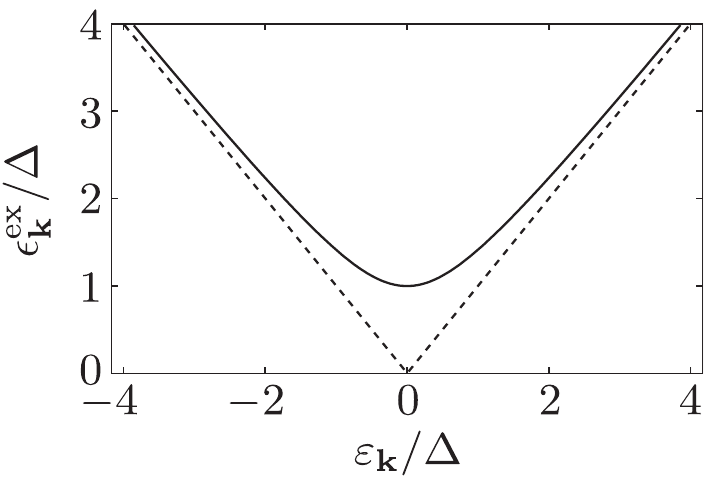
\includegraphics[width=0.5\textwidth]{immagini/Energia_eccitazione.png}
\end{figure}
\hspace{-0.6cm}Come possiamo vedere, se $\Delta=0$ si avrebbe una dispersione lineare. Se invece è presente l'interazione e quindi la superconduttività, l'energia delle eccitazioni è vicina a quella degli elettroni liberi quando $\xi_{\vb{k}} \gg \Delta$. Tuttavia, nella regione in cui $\xi_{\vb{k}} \ll \Delta$, cioè vicino allo zero dell'asse delle ascisse, il comportamento diventa completamente diverso: l'andamento è quadratico e, soprattutto, l'energia non si annulla mai. Esiste infatti un'energia minima necessaria per creare un'eccitazione, ed essa è proprio il gap energetico.\\
Più precisamente, se vogliamo rompere una coppia di Cooper, dobbiamo creare due stati eccitati, perché i due elettroni non vengono distrutti ma semplicemente trasformati in nuovi stati. Per questo motivo, quando parliamo di rottura di una coppia di Cooper, il costo energetico non è $\Delta$, bensì $2\Delta$, poiché è necessario separare entrambi gli elettroni della coppia.\\
Possiamo anche osservare come si comportino tutte le energie eccitate in funzione di $\vb{k}$:
\begin{figure}[H]
   \centering
   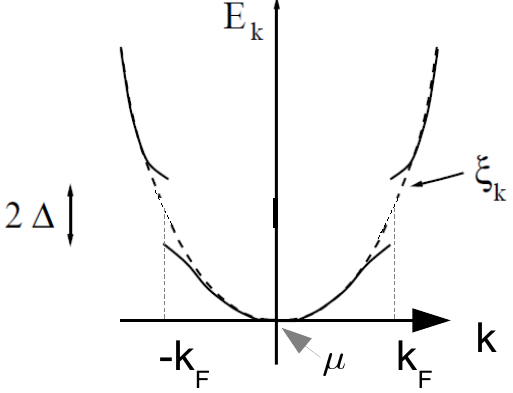
\includegraphics[width=0.5\textwidth]{immagini/Energia_eccitazione_rispetto_a_k.png}
\end{figure}
\hspace{-0.6cm}La linea tratteggiata rappresenta l'energia degli elettroni liberi, cioè l'energia degli elettroni in assenza di interazione:
\begin{equation*}
   E_{\vb{k}}
   =
   |\xi_{\vb{k}}|
   =
   \qty|
   \frac{\hbar^2 k^2}{2m}
   -
   \mu
   |
\end{equation*}
La linea continua rappresenta invece l'energia delle eccitazioni nello stato superconduttivo:
\begin{equation*}
   E_{\vb{k}}
   =
   \sqrt{
      \xi_{\vb{k}}^2
      +
      |\Delta|^2
   }
\end{equation*}
Osserviamo che in prossimità del vettore d'onda di Fermi compare un gap pari a $2\Delta$, perché gli elettroni che partecipano principalmente alla superconduttività sono proprio quelli vicini al livello di Fermi.\\
Abbiamo parlato di box di Nambu indipendenti; ciò significa che questi processi di eccitazione avvengono indipendentemente nei diversi box di Nambu. In questo senso possiamo interpretare tali eccitazioni come quasiparticelle non interagenti: ciascuna quasiparticella associata a un determinato box di Nambu non è direttamente collegata alle altre. Possiamo quindi usare il linguaggio delle quasiparticelle indipendenti nel senso che le eccitazioni presenti nei singoli box di Nambu risultano indipendenti tra loro.
\subsection{Condizione di autoconsistenza e gap energetico dipendente dalla temperatura}
Se vogliamo descrivere le proprietà che emergono da queste eccitazioni, cioè valutare le proprietà termodinamiche del sistema, dobbiamo considerare il fatto che tale sistema, nel quale sono presenti eccitazioni, si trova a temperatura finita. Il motivo per cui stiamo introducendo le eccitazioni è infatti capire cosa accade in un superconduttore a temperatura finita. Questo significa che dobbiamo determinare quale sia lo stato del sistema quando è presente una popolazione termica delle eccitazioni.\\
In generale, ciò viene descritto introducendo una matrice densità, esattamente nello stesso modo in cui si descrive un gas di Fermi normale a temperatura finita. Nel caso di un gas di Fermi normale, diciamo che le eccitazioni hanno energia $\varepsilon_{\vb{k}}$, e che il corrispondente stato è popolato con una probabilità legata all'occupazione termica; l'occupazione media è quindi espressa tramite la funzione di Fermi. Se vogliamo descrivere lo stato di tali particelle, dobbiamo considerare lo stato antisimmetrico rispetto allo scambio delle eccitazioni in equilibrio termico.\\
Qui dobbiamo fare esattamente la stessa cosa per queste quasiparticelle, poiché abbiamo visto che esse si comportano come gradi di libertà fermionici indipendenti in ciascun sottospazio. Se quindi vogliamo scrivere lo stato termico di queste particelle, dobbiamo introdurre una matrice densità della forma
\begin{equation*}
   W(T)
   =
   \frac{
      e^{-(H_{\rm MF}-\mu N_{\rm op})/k_B T}
   }{
      Z_{\rm MF}
   }
\end{equation*}
dove $Z_{\rm MF}$ è la funzione di partizione del sistema.\\
La probabilità di avere un'eccitazione è semplicemente data dalla funzione di Fermi, esattamente come nel caso di un normale gas di Fermi:
\begin{equation*}
   f(E^{\rm exc}_{\vb{k}})
   =
   \qty[
      1+
      e^{E^{\rm exc}_{\vb{k}}/k_B T}
   ]^{-1}
\end{equation*}
Quando abbiamo derivato lo stato fondamentale BCS, abbiamo ottenuto una condizione di autoconsistenza per $\Delta$ dalla quale abbiamo ricavato il modo in cui $\Delta$, cioè il gap a temperatura nulla, dipende dall'intensità dell'interazione. Quella era una condizione di autoconsistenza in cui il valor medio era calcolato rispetto allo stato fondamentale BCS.\\
Adesso abbiamo una nuova condizione di autoconsistenza. Essa emerge matematicamente dal sistema di equazioni lineari che abbiamo appena derivato per esprimere l'energia delle eccitazioni. Si tratta sostanzialmente dello stesso tipo di condizione di autoconsistenza; l'unica differenza è che ora i valori medi sui due membri dell'equazione vengono valutati rispetto allo stato di equilibrio termico che tiene conto delle eccitazioni.\\
Questo significa che il valor medio di $Z$ non è altro che il valor medio della combinazione di operatori che lo definisce. Poiché $Z$ è una combinazione di due operatori di creazione, dobbiamo esprimere tali operatori in termini dei nuovi operatori fermionici e poi valutare il valor medio di questa combinazione nello stato di equilibrio termico. Scriviamo quindi
\begin{equation*}
   \Delta(T)
   =
   V
   \sum_{\vb{k}}
   u^*_{\vb{k}}
   \nu_{\vb{k}}
   \expval*{Z_{\vb{k}}}
\end{equation*}
ossia\mn{Quello che stiamo facendo implicitamente è sostituire $Z_{\vb{k}}$ con la sua espressione in termini degli operatori di creazione e annichilazione, e poi esprimere questi ultimi in termini dei nuovi operatori fermionici $b$ invertendo la trasformazione di Bogoliubov--Valatin, trascurando i termini del tipo $b b$ e $b^\dag b^\dag$.}
\begin{equation*}
   \Delta(T) = V \sum_{\vb{k}} u^*_{\vb{k}} \nu_{\vb{k}} \expval*{ \bigl(1 - b^{\dag}_{\vb{k},\uparrow} b^{\vphantom{\dag}}_{\vb{k},\uparrow} -  b^{\dag}_{-\vb{k},\downarrow} b^{\vphantom{\dag}}_{-\vb{k},\downarrow} \bigr) }
\end{equation*}
I valori medi di queste combinazioni di operatori, $\expval*{b^{\dag}_{\vb{k},\uparrow} b^{\vphantom{\dag}}_{\vb{k},\uparrow}}$ e $\expval*{b^{\dag}_{-\vb{k},\downarrow} b^{\vphantom{\dag}}_{-\vb{k},\downarrow}}$, sono legati alla probabilità di trovare l'eccitazione rispettivamente negli stati $(\vb{k},\uparrow)$ e $(-\vb{k},\downarrow)$. Poiché tali quasiparticelle obbediscono alla statistica di Fermi-Dirac, si ha 
\begin{equation*}
   \expval*{b^{\dag}_{\vb{k},\uparrow} b^{\vphantom{\dag}}_{\vb{k},\uparrow}}
   =\expval*{b^{\dag}_{-\vb{k},\downarrow} b^{\vphantom{\dag}}_{-\vb{k},\downarrow}}
   =f(E_{\vb{k}})
\end{equation*}
Pertanto, la condizione di autoconsistenza per $\Delta$ assume la forma
\begin{equation*}
   \Delta(T)
   = V \sum_{\vb{k}} u^*_{\vb{k}} \nu_{\vb{k}} \bigl[ 1 - 2f(E_{\vb{k}}) \bigr]
   = V \sum_{\vb{k}} u^*_{\vb{k}} \nu_{\vb{k}} \tanh \qty( \frac{\beta E^{\rm exc}_{\vb{k}}}{2} )
\end{equation*}
Se adesso utilizziamo la relazione
\begin{equation*}
   u^*_{\vb{k}}
   \nu_{\vb{k}}
   =
   \frac{1}{2}
   \frac{
      \Delta
   }{
      \sqrt{
         \xi^2_{\vb{k}}
         +
         |\Delta|^2
      }
   }
\end{equation*}
la condizione di autoconsistenza per $\Delta$ assume la forma
\begin{equation*}
   \Delta(T)
   =
   \frac{|V|}{2}
   \sum_{\vb{k}}
   \frac{
      \Delta(T)
   }{
      \sqrt{
         \xi^2_{\vb{k}}
         +
         |\Delta|^2
      }
   }
   \tanh \qty[
      \frac{
         \beta
         \sqrt{
            \xi^2_{\vb{k}}
            +
            \Delta(T)^2
         }
      }{2}
   ]
\end{equation*}
Questa equazione è sostanzialmente la stessa ottenuta nel caso a temperatura nulla, tranne per il contributo aggiuntivo dipendente dalla temperatura.\\
Anche in questo caso la condizione può essere espressa come un integrale sull'energia, passando al limite del continuo e introducendo la densità degli stati:
\begin{equation*}
   1
   =
   \frac{|V|N(0)}{2}
   \int
   \dd{\xi}
   \frac{
      \tanh \qty(
         \beta
         \sqrt{
            \xi^2+\Delta(T)^2
         }/2
      )
   }{
      \sqrt{
         \xi^2+|\Delta|^2
      }
   }
\end{equation*}
A temperatura nulla otteniamo ciò che avevamo già trovato:
\begin{equation*}
   \Delta(0)
   =
   2\hbar\omega_D
   e^{-1/|V|N(0)}
\end{equation*}
mentre alla temperatura critica accade che $\Delta(T)\to0$. In questo caso, $E_{\vb{k}} \to |\xi_{\vb{k}}|$ e lo spettro delle eccitazioni diventa uguale a quello dello stato normale. Di conseguenza, $T_c$ si ottiene sostituendo $E_{\vb{k}}$ con $|\xi_{\vb{k}}|$ nell'equazione precedente:
\begin{equation}
   \frac{1}{|V|}
   =
   \frac{N(0)}{2}
   \int_{-\hbar\omega_D}^{\hbar\omega_D}
   \dd{\xi}
   \,
   \tanh\qty(
      \frac{\xi}{2k_B T_c}
   )
   \frac{1}{\xi}
   \label{eq:critical_temperature_integral}
\end{equation}
Questo integrale può essere risolto analiticamente. In particolare si può mostrare che
\begin{equation*}
   \frac{1}{|V|}
   =
   N(0)
   \ln\qty(
      2e^{\gamma}
      \frac{
         \hbar\omega_D
      }{
         \pi k_B T_c
      }
   )
\end{equation*}
e ciò permette di collegare la temperatura critica ai parametri che caratterizzano il superconduttore, in particolare l'intensità dell'interazione, la densità degli stati e l'energia di Debye. Invertendo questa relazione otteniamo
\begin{equation*}
   k_B T_c
   =
   \frac{
      2e^{\gamma}
   }{
      \pi
   }
   \hbar\omega_D
   e^{-1/N(0)|V|}
\end{equation*}
Possiamo ora confrontare il gap energetico a temperatura nulla con l'espressione della temperatura critica. Confrontando le due formule si trova infatti una relazione diretta tra queste quantità:
\begin{equation*}
   \Delta(0)
   \sim
   \frac{2}{A}
   k_B T_c
   \sim
   1.764\,k_B T_c
\end{equation*}
Il coefficiente numerico dipende dalle proprietà del materiale, ma per la maggior parte dei superconduttori di tipo I assume proprio questo valore.\\
Vediamo ora l'andamento del gap in funzione della temperatura. La quantità $\Delta(T)$ può essere calcolata numericamente a partire dall'\eqrefcustom{eq:critical_temperature_integral}. Per i superconduttori in regime di accoppiamento debole, nei quali $\hbar\omega_c/k_B T_c \gg 1$, il rapporto $\Delta(T)/\Delta(0)$ è una funzione universale di $T/T_c$ che decresce monotonicamente da $1$ a $T=0$ fino a $0$ a $T=T_c$, come mostrato nella figura seguente:
\begin{figure}[H]
   \centering
   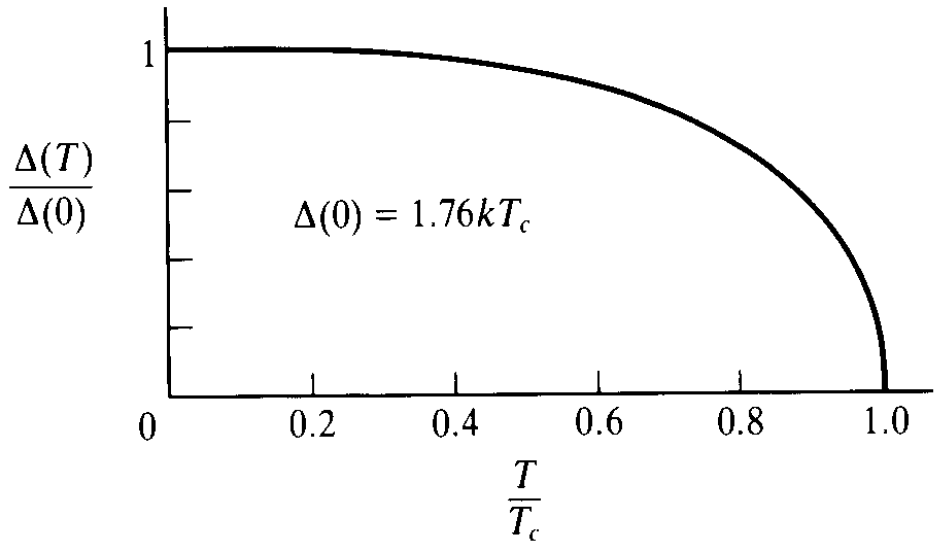
\includegraphics[width=0.6\textwidth]{immagini/Gap_temperature_dependence.png}
\end{figure}
\hspace{-0.6cm}Vicino a $T=0$, la variazione con la temperatura è esponenzialmente lenta, poiché $e^{-\Delta/k_B T} \approx 0$, così che la tangente iperbolica è praticamente uguale a $1$ e quasi indipendente dalla temperatura. Dal punto di vista fisico, ciò significa che $\Delta$ rimane quasi costante finché un numero significativo di quasiparticelle non viene eccitato termicamente.\\
Al contrario, per $T\simeq T_c$, il gap $\Delta(T)$ si annulla con tangente verticale, approssimativamente secondo la legge
\begin{equation*}
   \frac{\Delta(T)}{\Delta(0)}
   \approx 1.74 \qty( 1-\frac{T}{T_c} )^{1/2}
\end{equation*}
La dipendenza del parametro d'ordine $\Delta$ dalla radice quadrata di $(T_c-T)$ è una caratteristica generale di tutte le teorie di campo medio.
\subsection{Quantità termodinamiche}
Passiamo adesso alle proprietà termodinamiche. Abbiamo ormai tutti gli ingredienti necessari, poiché conosciamo $\Delta$, che dipende dalla temperatura.\\
Prima di procedere facciamo un passo indietro. Quando in meccanica quantistica abbiamo un'Hamiltoniana e la diagonalizziamo, otteniamo gli autostati e le autenergie $E_n$, che dipendono soltanto dai parametri dell'Hamiltoniana. Sappiamo poi che, a temperatura finita, la probabilità di trovare, ad esempio nel caso di una singola particella, il sistema in un autostato di energia $E_n$ è legata a $e^{-\beta E_n}$ nella combinazione appropriata, a seconda che le particelle siano fermioniche oppure bosoniche. Il punto importante è quindi che le autenergie dipendono soltanto dai parametri dell'Hamiltoniana.\\
Qui però abbiamo qualcosa di più sottile. Infatti, è vero che nel box di Nambu $\vb{k}$ abbiamo ottenuto delle energie $E_{\vb{k}}$ che dipendono da $\xi_{\vb{k}}$ e da $\Delta$, cioè da quantità legate ai parametri originari dell'Hamiltoniana; tuttavia, quando abbiamo imposto la condizione di autoconsistenza, abbiamo ottenuto un $\Delta$ dipendente dalla temperatura. Questo significa che ora le energie di eccitazione dipendono anch'esse dalla temperatura.\\
Il motivo per cui stiamo considerando energie di eccitazione dipendenti dalla temperatura è che dobbiamo includere questo parametro $\Delta(T)$, il quale dipende dalla temperatura proprio perché deve soddisfare la condizione di autoconsistenza derivante dall'approssimazione di campo medio introdotta in precedenza.\\
Le proprietà termodinamiche che vogliamo descrivere includono quindi un gap dipendente dalla temperatura direttamente nelle autenergie. Esse derivano essenzialmente dal considerare un gas di quasiparticelle fermioniche con numeri di occupazione dati dalla funzione di Fermi:
\begin{equation*}
   f_{\vb{k}}
   =\bigl[ 1+e^{\beta E_{\vb{k}}} \bigr]^{-1}
   \qq{dove}
   E_{\vb{k}}
   =
   \sqrt{ \xi_{\vb{k}}^2 + |\Delta(T)|^2 }
\end{equation*}
La peculiarità è che la temperatura non compare soltanto in $\beta$, ma entra anche direttamente nell'energia attraverso $\Delta(T)$.\\
Una volta compreso come trattare queste eccitazioni, possiamo utilizzare le usuali relazioni termodinamiche valide per un gas fermionico, espresse in termini dei numeri di occupazione. L'unica differenza è che tali numeri di occupazione dipendono dalle energie di eccitazione che abbiamo derivato, e che determinano a loro volta l'entropia elettronica nel modo usuale per un gas fermionico:
\begin{equation}
   S_{es}=-2k_B \sum_{\vb{k}} \Big[ (1-f_{\vb{k}}) \ln(1-f_{\vb{k}}) + f_{\vb{k}} \ln f_{\vb{k}} \Big]
   \label{eq:entropy}
\end{equation}
Una volta nota $S_{es}(T)$, il calore specifico può essere scritto come
\begin{equation}
   C_{es}
   =
   T\dv{S_{es}}{T}
   =
   -\beta\dv{S_{es}}{\beta}
   \label{eq:specific_heat_def}
\end{equation}
Usando l'\eqrefcustom{eq:entropy}, otteniamo
\begin{equation}
   \begin{split}
      C_{es}
      &= 2\beta k_B \sum_{\vb{k}} \pdv{f_{\vb{k}}}{\beta} \ln\qty( \frac{f_{\vb{k}}}{1 - f_{\vb{k}}} )\\
      &= -2\beta^2 k_B \sum_{\vb{k}} E_{\vb{k}} \pdv{f_{\vb{k}}}{\beta}
      \\
      &=
      -2\beta^2 k_B
      \sum_{\vb{k}}
      E_{\vb{k}}
      \frac{
         df_{\vb{k}}
      }{
         d(\beta E_{\vb{k}})
      }
      \qty(
         E_{\vb{k}}
         +
         \beta
         \frac{dE_{\vb{k}}}{d\beta}
      )
      \\
      &=
      2\beta k_B
      \sum_{\vb{k}}
      \frac{\partial f_{\vb{k}}}{\partial E_{\vb{k}}}
      \qty(
         E_{\vb{k}}^2
         +
         \frac{1}{2}
         \beta
         \frac{d\Delta^2}{d\beta}
      )
   \end{split}
   \label{eq:specific_heat_final}
\end{equation}
Il primo termine è quello usuale e deriva dalla ridistribuzione delle quasiparticelle tra i vari livelli energetici al variare della temperatura. Il secondo termine è invece più particolare e descrive l'effetto della dipendenza del gap dalla temperatura nel modificare direttamente i livelli energetici stessi.\\
Consideriamo ora questa espressione in due limiti. Il primo è il caso molto vicino alla temperatura critica $T_c$, dove $\Delta(T)\to0$ ed $E_{\vb{k}}$ si riduce a $\xi_{\vb{k}}$. In questo limite, il primo termine coincide con il normale calore specifico elettronico dello stato normale, $C_{en}=\gamma T$, che è continuo in $T_c$.\\
Il secondo termine invece è finito al di sotto di $T_c$, dove $\dv*{\Delta^2}{T}$ è grande, mentre è nullo al di sopra di $T_c$. Questo dà origine a una discontinuità $\Delta C$ nel calore specifico elettronico in corrispondenza di $T_c$. Si tratta del risultato che avevamo già introdotto all'inizio, ma che ora comprendiamo a partire dalla derivazione delle energie di eccitazione e della condizione di autoconsistenza, che introduce una dipendenza dalla temperatura anche nelle energie stesse.\\
Si può mostrare che l'ampiezza della discontinuità è
\begin{equation*}
   \Delta C
   =
   9.4\,N(0)k_B^2T_c
\end{equation*}
L'andamento complessivo del calore specifico elettronico è illustrato nella figura seguente:
\begin{figure}[H]
   \centering
   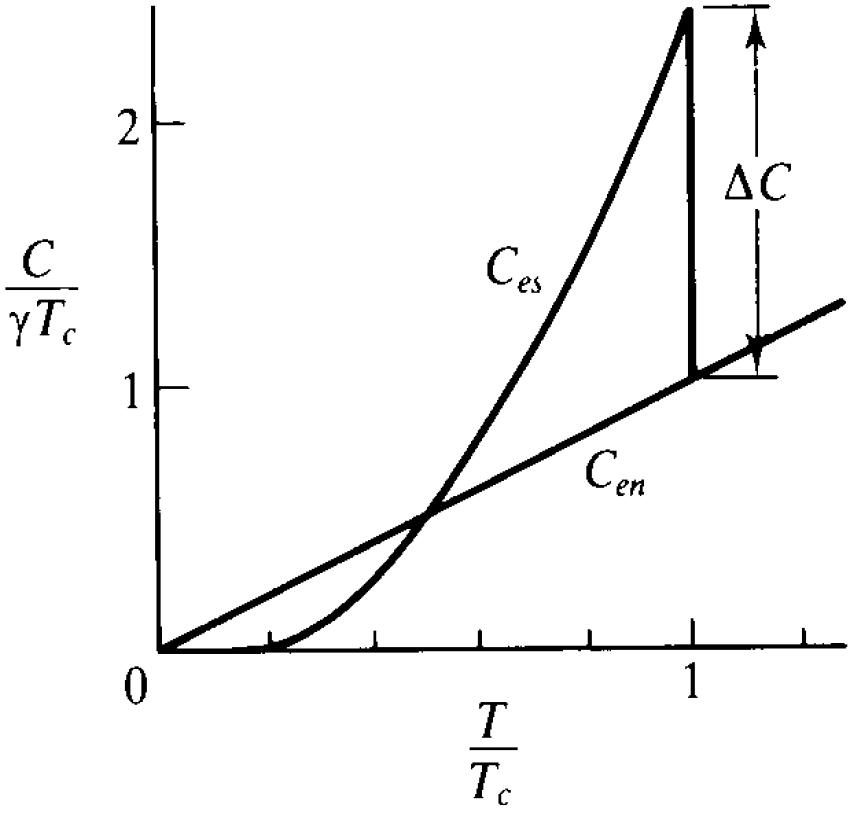
\includegraphics[width=0.5\textwidth]{immagini/Specific_heat.png}
\end{figure}
\hspace{-0.6cm}Consideriamo adesso il limite di temperature molto basse. In questo caso possiamo approssimare la funzione di Fermi con un comportamento esponenziale:
\begin{equation*}
   f_{\vb{k}}
   \approx
   e^{-E_{\vb{k}}/k_B T}
\end{equation*}
Abbiamo già osservato che a basse temperature è sempre presente un gap nello spettro, quindi possiamo descrivere le proprietà a bassa temperatura considerando il valore minimo del gap energetico, cioè $\Delta$. Inoltre abbiamo già visto che questo gap è proporzionale alla temperatura critica, quindi:
\begin{equation*}
   f_{\vb{k}}
   \approx
   e^{-\Delta/k_B T}
   =
   e^{-bT_c/T}
\end{equation*}
È evidente che, nel limite $T\ll T_c$, entrambi i termini in $C_{es}$ risultano esponenzialmente piccoli, poiché l'energia minima di eccitazione $\Delta$ è molto maggiore di $k_B T$. Questo spiega il comportamento esponenziale del calore specifico a basse temperature in un superconduttore:
\begin{equation*}
   C_{es}
   =
   \gamma T_c
   a
   e^{-bT_c/T}
\end{equation*}
Il fatto che il calore specifico sia non solo più piccolo, ma addirittura inferiore rispetto a quello di un metallo normale, deriva proprio dal comportamento della funzione di Fermi a basse temperature in presenza di un gap nello spettro. Più precisamente, tale andamento esponenziale discende direttamente dal comportamento esponenziale della funzione di Fermi.\\
Questi due regimi limite, temperatura nulla e temperatura critica, possono quindi essere compresi considerando la dipendenza delle autenergie dal gap superconduttivo e, più in generale, dalla temperatura.\\
Possiamo infine considerare anche le altre proprietà termodinamiche elettroniche, in particolare l'entropia, l'energia interna e l'energia libera di Helmholtz:
\begin{equation*}
   \begin{split}
      C_{el}
      & = T\dv{S_{es}}{T}
      = -\beta\dv{S_{es}}{\beta}
      \\
      F_{es}(T)
      & = U_{es}(T) - TS_{es}(T)
   \end{split}
\end{equation*}
\begin{figure}[H]
   \centering
   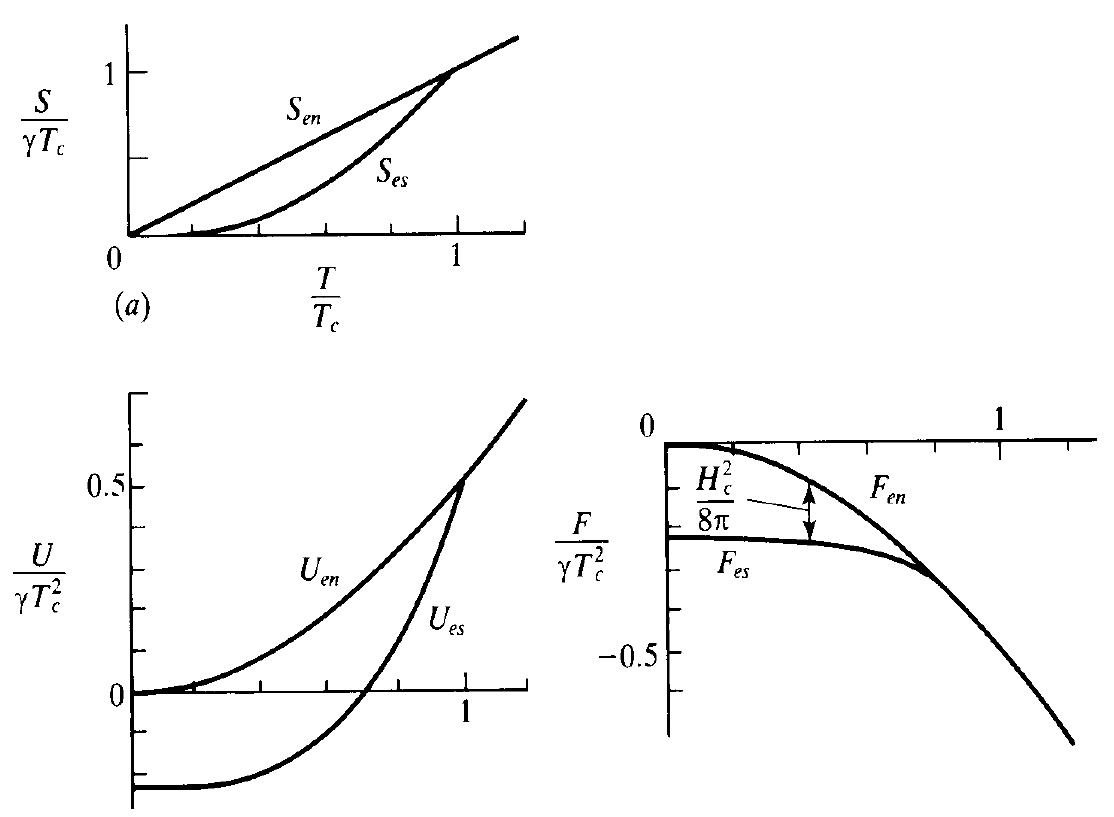
\includegraphics[width=0.9\textwidth]{immagini/Other_thermodynamic_quantities.png}
\end{figure}
\hspace{-0.6cm}Questi andamenti emergono immediatamente osservando la dipendenza dalla temperatura di tali quantità attraverso le energie di eccitazione. In particolare, in tutti questi casi non compare alcuna discontinuità, il che spiega perché la transizione superconduttiva a temperatura finita sia una transizione di fase del secondo ordine. Anche questo risultato emerge naturalmente dalla derivazione microscopica.
\subsection{Energie di eccitazione e densità degli stati}
Abbiamo visto che le energie di eccitazione assumono la forma
\begin{equation*}
   E_{\vb{k}}
   =
   \sqrt{
      \xi_{\vb{k}}^2
      +
      |\Delta|^2
   }
\end{equation*}
e che, per piccoli valori di $\xi_{\vb{k}}$, la dipendenza dall'energia è quadratica. Inoltre, per $\xi_{\vb{k}}=0$ compare un intervallo energetico nel quale le eccitazioni non possono esistere, cioè il gap che abbiamo già introdotto.\\
Abbiamo anche visto che tali eccitazioni vengono create e distrutte dagli operatori fermionici $b_{\vb{k},\uparrow}$ e $b^{\dag}_{\vb{k},\uparrow}$, che sono in corrispondenza biunivoca con gli operatori di creazione e distruzione degli elettroni ordinari $c_{\vb{k},\uparrow}$ e $c^{\dag}_{\vb{k},\uparrow}$, nel senso che sono legati a essi tramite trasformazioni lineari.\\
Questa corrispondenza implica che, se vogliamo valutare la densità degli stati di queste eccitazioni, possiamo assumere che esse abbiano una densità $N_s(E)$ tale che il numero di eccitazioni comprese nell'intervallo energetico $\dd{E}$, cioè $N_s(E)\dd{E}$, corrisponda esattamente al numero di stati elettronici normali con energia compresa nell'intervallo $\dd{\xi}$. In altre parole, dobbiamo uguagliare il numero di stati del superconduttore al numero di stati del metallo normale:
\begin{equation*}
   N_s(E)\dd{E}=N_n(\xi)\dd{\xi}
\end{equation*}
Questi numeri coincidono proprio grazie alla corrispondenza tra gli operatori fermionici dei due problemi.\\
Questa identità permette di ricavare molto facilmente la densità degli stati del superconduttore. Infatti possiamo riscriverla come
\begin{equation*}
   \frac{ N_s(E) }{
      N_n(\xi)
   }
   =
   \dv{\xi}{E}
\end{equation*}
Poiché siamo interessati principalmente a energie $\xi$ che differiscono dal livello di Fermi solo di pochi meV, possiamo approssimare la densità degli stati normale come costante:
\begin{equation*}
   N_n(\xi)\approx N(0)
\end{equation*}
Inoltre, dato che conosciamo esplicitamente la dipendenza di $\xi$ da $E$, possiamo calcolare la derivata e ottenere
\begin{equation*}
   \frac{ N_s(E)}{N_n(\xi)}
   =
   \begin{dcases}
      \frac{E}{\sqrt{ E^2 -|\Delta|^2}}
      & \text{per } E>\Delta
      \\[0.3cm]
      0
      & \text{per } E<\Delta
   \end{dcases}
\end{equation*}
La densità degli stati delle eccitazioni si annulla quindi per energie inferiori al gap, come è naturale aspettarsi dato che abbiamo visto che in quella regione non esistono eccitazioni. Per energie superiori a $\Delta$, invece, la densità degli stati deriva semplicemente dalla derivata di $\xi$ rispetto a $E$.\\
Possiamo rappresentare graficamente questa densità degli stati:
\begin{figure}[H]
   \centering
   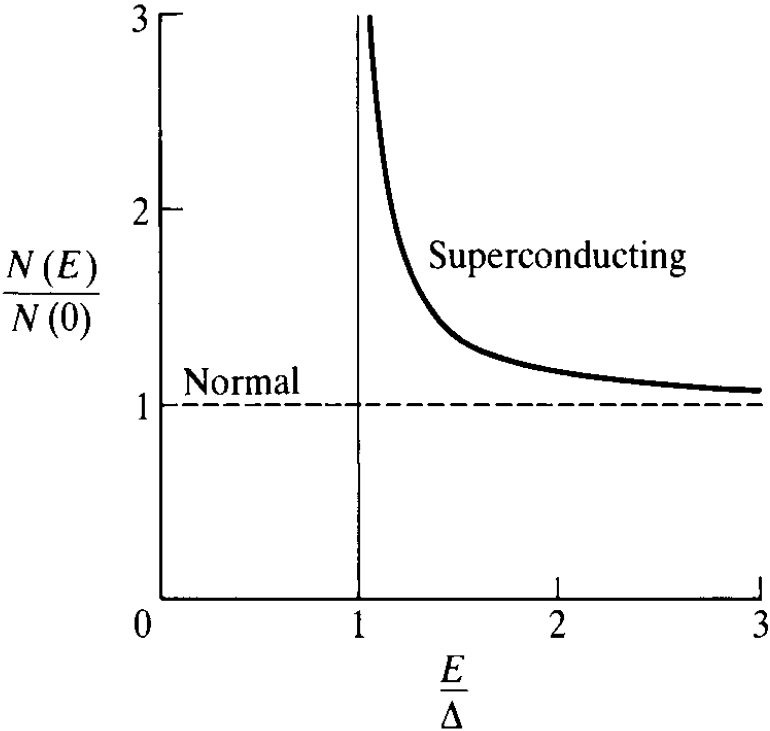
\includegraphics[width=0.5\textwidth]{immagini/Density_of_states.png}
\end{figure}
\hspace{-0.6cm}Come si vede, la densità degli stati è nulla per energie inferiori al gap, cioè per $E/\Delta<1$. Per energie molto maggiori di $\Delta$, essa tende invece al valore del metallo normale. Infatti, nel limite $E\gg\Delta$, si ha
\begin{equation*}
   \frac{
      E
   }{
      \sqrt{
         E^2-|\Delta|^2
      }
   }
   \approx
   \frac{
      E
   }{
      \sqrt{E^2}
   }
   =
   1
\end{equation*}
Nel limite $E\to\Delta$, cioè quando $E/\Delta \to 1$, il denominatore tende a zero e compare quindi una divergenza della densità degli stati in prossimità del gap.\\
La densità degli stati di un superconduttore presenta quindi tre caratteristiche fondamentali:
\begin{itemize}[leftmargin=0.5cm]
   \item è nulla per energie inferiori al gap;
   \item tende alla densità degli stati del metallo normale per energie molto maggiori del gap;
   \item presenta una divergenza in corrispondenza del bordo del gap.
\end{itemize}
Quest'ultimo comportamento riflette il fatto che, vicino al gap, gli stati di eccitazione si accumulano fortemente.
\subsection{Elettrodinamica dei superconduttori BCS}
Vediamo ora quali siano le conseguenze di questa densità degli stati.\\
Consideriamo la risposta a un campo magnetico statico. Supponiamo quindi di avere un campo magnetico $\vb{B}$ generato da un potenziale vettore $\vb{A}$.\\
Quello che vogliamo capire è innanzitutto quale sia l'effetto della presenza di un campo magnetico sull'Hamiltoniana complessiva del sistema, dato che finora abbiamo considerato l'Hamiltoniana BCS in assenza di campo magnetico. Come facciamo? Dobbiamo considerare il modo in cui il campo magnetico influenza il sistema elettronico.\\
Sappiamo che, in generale, per particelle con momento $\vb{p}$ e carica $e$, il momento viene sostituito con il momento gauge-invariante:
\begin{equation*}
   \vb{p}
   \to
   \vb{p}
   -
   \frac{e}{c}\vb{A}
\end{equation*}
Questo significa che il termine cinetico dell'Hamiltoniana viene modificato nel modo seguente:
\begin{equation*}
   \frac{\vb{p}^2}{2m}
   \to
   \frac{1}{2m}
   \qty(
      \vb{p}
      -
      \frac{e}{c}\vb{A}
   )^2
\end{equation*}
ossia
\begin{equation*}
   \frac{1}{2m}
   \qty(
      \vb{p}
      -
      \frac{e}{c}\vb{A}
   )^2
   =
   \frac{1}{2m}
   \qty(
      \vb{p}^2
      +
      \frac{e^2}{c^2}\vb{A}^2
      -
      \frac{e}{c}\vb{p}\vdot\vb{A}
      -
      \frac{e}{c}\vb{A}\vdot\vb{p}
   )
\end{equation*}
Poiché siamo interessati soltanto alla risposta lineare a campi deboli, manteniamo solo i termini lineari in $\vb{A}$ e trascuriamo quindi il termine proporzionale a $\vb{A}^2$.\\
Esprimendo l'operatore $\vb{p}$ come $-i\hbar\grad$,il termine cinetico diventa
\begin{equation*}
   \frac{1}{2m}
   \qty(
      \vb{p}
      -
      \frac{e}{c}\vb{A}
   )^2
   =
   \frac{\vb{p}^2}{2m}
   +
   i\hbar\frac{e}{2mc}\div{\vb{A}}
   +
   i\hbar\frac{e}{2mc}\vb{A}\vdot\grad
\end{equation*}
Se scegliamo la gauge di London, per cui
\[
\div{\vb{A}}=0,
\]
il secondo termine si annulla e rimane\mn{Sono abbastanza convinto che questa parte sia sbagliata e che in realtà i due termini si possano sommare.}
\begin{equation*}
   \frac{1}{2m}
   \qty(
      \vb{p}
      -
      \frac{e}{c}\vb{A}
   )^2
   =
   \frac{\vb{p}^2}{2m}
   +
   i\frac{e\hbar}{mc}\vb{A}\vdot\grad
\end{equation*}
Il passo successivo consiste nel capire come questo termine perturbativo possa essere scritto in seconda quantizzazione, cioè esplicitamente in termini di operatori di creazione e distruzione elettronici.\\
Per farlo dobbiamo vedere come tale termine agisce sulle onde piane corrispondenti a uno stato con momento $\vb{k}$. Abbiamo
\begin{equation*}
   \vb{A}\vdot\grad
   e^{i\vb{k}\vdot\vb{r}}
   =
   i\vb{A}\vdot\vb{k}
   e^{i\vb{k}\vdot\vb{r}}
\end{equation*}
Questo significa che, se vogliamo trovare la rappresentazione di questo termine di interazione nella base delle onde piane, dobbiamo utilizzare l'azione del gradiente sulle onde piane. Inoltre, conviene espandere il potenziale vettore in trasformata di Fourier:
\begin{equation*}
   \vb{A}(\vb{r})
   =
   \sum_{\vb{q}}
   \vb{a}(\vb{q})
   e^{i\vb{q}\vdot\vb{r}}
\end{equation*}
Il termine di interazione assume allora la forma
\begin{equation*}
   V
   =
   i\frac{e \hbar}{mc}
   \sum_{\vb{k}}
   \sum_{\vb{q}}
   \vb{a}(\vb{q})
   \vdot
   i\vb{k}
   e^{i(\vb{q}+\vb{k})\vdot\vb{r}}
\end{equation*}
Cerchiamo di capire il significato fisico di questa espressione. L'idea è che, se questo termine di interazione agisce su un'elettrone con momento $\vb{k}$, esso ne modifica il momento in $\vb{k}+\vb{q}$.\\
Questo significa che l'interazione descrive un processo di scattering in cui un elettrone con momento $\vb{k}$ viene trasformato in uno stato con momento $\vb{k}+\vb{q}$ senza modificarne lo spin.\\
Di conseguenza, l'operatore di seconda quantizzazione che descrive tale processo deve distruggere un elettrone con momento $\vb{k}$ e crearne uno con momento $\vb{k}+\vb{q}$. Si ottiene quindi
\begin{equation*}
   V
   =
   -
   \frac{e \hbar}{mc}
   \sum_{\vb{k}}
   \sum_{\vb{q}}
   \sum_{\sigma}
   \vb{a}(\vb{q})
   \vdot
   \vb{k}
   \,
   c^{\dag}_{\vb{k}+\vb{q},\sigma}
   c^{\vphantom{\dag}}_{\vb{k},\sigma}
\end{equation*}
Questa è quindi la forma del termine aggiuntivo che deve essere incluso nell'Hamiltoniana BCS quando si considera l'azione di un campo magnetico esterno.\\
A questo punto introduciamo un'approssimazione. Finora $\vb{a}(\vb{q})$ contiene tutti i possibili momenti, cioè stiamo considerando un potenziale vettore completamente generico. L'idea ora è quella di considerare il regime in cui il campo magnetico è quasi uniforme all'interno del superconduttore. Questo significa che anche le variazioni spaziali del potenziale vettore sono molto lente e quindi sono rilevanti soltanto valori piccoli di $\vb{q}$.\\
Possiamo quindi sostituire
\[
\vb{a}(\vb{q})
\to
\vb{a}(0),
\]
effettuando quella che viene chiamata \emph{approssimazione a grande lunghezza d'onda}. In questa approssimazione l'interazione si semplifica ulteriormente:
\begin{equation*}
   V
   \simeq
   -
   \frac{e \hbar}{mc}
   \sum_{\vb{k}}
   \sum_{\sigma}
   \vb{a}(0)\vdot\vb{k}
   \,
   c^{\dag}_{\vb{k},\sigma}
   c^{\vphantom{\dag}}_{\vb{k},\sigma}
\end{equation*}
Ricordiamo ora che gli operatori $c_{\vb{k},\sigma}$ sono legati agli operatori $b_{\vb{k},\uparrow}$ e $b_{-\vb{k},\downarrow}$ attraverso la trasformazione di Bogoliubov. Possiamo quindi riscrivere il termine di interazione in funzione degli operatori che creano e distruggono le eccitazioni del superconduttore. Invertendo l'\eqrefcustom{eq:Bogoliubov_Valatin_transformation_explicit}, si ottiene
\begin{equation*}
   V = - \frac{e \hbar}{2mc} \sum_{\vb{k}} \vb{a}(0)\vdot\vb{k} \qty[ b^{\dag}_{\vb{k},\uparrow} b^{\vphantom{\dag}}_{\vb{k},\uparrow} - b^{\dag}_{-\vb{k},\downarrow} b^{\vphantom{\dag}}_{-\vb{k},\downarrow} ]
\end{equation*}
L'Hamiltoniana BCS complessiva diventa quindi
\begin{equation*}
   H_{\rm BCS} = \sum_{\vb{k},\sigma} E_{\vb{k}} b^{\dag}_{\vb{k},\sigma} b^{\vphantom{\dag}}_{\vb{k},\sigma} - \frac{e \hbar}{2mc} \sum_{\vb{k}} \vb{a}(0)\vdot\vb{k} \qty[ b^{\dag}_{\vb{k},\uparrow} b^{\vphantom{\dag}}_{\vb{k},\uparrow} - b^{\dag}_{-\vb{k},\downarrow} b^{\vphantom{\dag}}_{-\vb{k},\downarrow} ]
\end{equation*}
Osserviamo che questa Hamiltoniana è ancora diagonale. Possiamo quindi scriverla come
\begin{equation*}
   H_{\rm BCS}
   =
   \sum_{\vb{k},\sigma}
   \tilde{E}_{\vb{k}}
   b^{\dag}_{\vb{k},\sigma}
   b^{\vphantom{\dag}}_{\vb{k},\sigma}
\end{equation*}
dove
\begin{equation*}
   \begin{split}
      \tilde{E}_{\vb{k},\uparrow}
      &=
      E_{\vb{k},\uparrow}
      -
      \frac{e\hbar}{mc}
      \vb{a}(0)\vdot\vb{k}
      =
      E_{\vb{k},\uparrow}
      -
      \delta
      \\[0.2cm]
      \tilde{E}_{-\vb{k},\downarrow}
      &=
      E_{-\vb{k},\downarrow}
      +
      \frac{e\hbar}{mc}
      \vb{a}(0)\vdot\vb{k}
      =
      E_{-\vb{k},\downarrow}
      +
      \delta
   \end{split}
\end{equation*}
Una volta scritta esplicitamente l'Hamiltoniana modificata, vogliamo determinare la risposta elettromagnetica del superconduttore, cioè la densità di corrente. L'obiettivo finale è ottenere una relazione tra la corrente e il potenziale vettore e recuperare eventualmente l'equazione di London con una forma esplicita della lunghezza di penetrazione.\\
Il punto di partenza è scrivere la densità di corrente:
\begin{equation*}
   \vb{J}
   =
   \frac{ne}{m}\vb{p}
   -
   \frac{ne^2}{mc}\vb{A}
   =
   \vb{J}_1+\vb{J}_2
\end{equation*}
Il termine $\vb{J}_1$ è detto termine paramagnetico, mentre $\vb{J}_2$ è il termine diamagnetico.\\
Scriviamo esplicitamente $\vb{J}_1$. Sostituendo
\[
\vb{p}\to -i\hbar\grad
\]
e considerando l'azione sulle onde piane:
\begin{equation*}
   \vb{p}
   e^{i\vb{k}\vdot\vb{r}}
   =
   -i\hbar
   \grad
   e^{i\vb{k}\vdot\vb{r}}
   =
   \hbar\vb{k}
   e^{i\vb{k}\vdot\vb{r}}
\end{equation*}
Otteniamo quindi
\begin{equation*}
   \vb{J}_1
   =
   \frac{ne\hbar}{m}
   \sum_{\vb{k},\sigma}
   \vb{k}
   c^{\dag}_{\vb{k},\sigma}
   c^{\vphantom{\dag}}_{\vb{k},\sigma}
\end{equation*}
ossia
\begin{equation*}
   \vb{J}_1
   =
   \frac{ne\hbar}{m}
   \sum_{\vb{k}}
   \vb{k}
   \qty[
      b^{\dag}_{\vb{k},\uparrow}
      b^{\vphantom{\dag}}_{\vb{k},\uparrow}
      -
      b^{\dag}_{\vb{k},\downarrow}
      b^{\vphantom{\dag}}_{\vb{k},\downarrow}
   ]
\end{equation*}
Per il termine diamagnetico utilizziamo invece lo sviluppo di Fourier del potenziale vettore:
\begin{equation*}
   \vb{J}_2
   =
   -
   \frac{ne^2}{mc}
   \sum_{\vb{q}}
   \vb{a}(\vb{q})
   e^{i\vb{q}\vdot\vb{r}}
\end{equation*}
Nell'approssimazione a grande lunghezza d'onda:
\begin{equation*}
   \vb{J}_2
   \simeq
   -
   \frac{ne^2}{mc}
   \vb{a}(0)
\end{equation*}
A questo punto vogliamo valutare il valor medio termico della corrente a temperatura finita ma inferiore a $T_c$. Iniziamo con $\expval*{\vb{J}_1}$:
\begin{equation*}
   \expval*{\vb{J}_1}
   =
   \frac{ne\hbar}{m}
   \sum_{\vb{k}}
   \vb{k}
   \qty[
      \expval*{
         b^{\dag}_{\vb{k},\uparrow}
         b^{\vphantom{\dag}}_{\vb{k},\uparrow}
      }
      -
      \expval*{
         b^{\dag}_{\vb{k},\downarrow}
         b^{\vphantom{\dag}}_{\vb{k},\downarrow}
      }
   ]
\end{equation*}
Questi valori medi non sono altro che le occupazioni termiche fermioniche delle quasiparticelle, quindi
\begin{equation*}
   \expval*{
      b^{\dag}_{\vb{k},\uparrow}
      b^{\vphantom{\dag}}_{\vb{k},\uparrow}
   }
   =
   f(\tilde{E}_{\vb{k},\uparrow})
\end{equation*}
e
\begin{equation*}
   \expval*{
      b^{\dag}_{\vb{k},\downarrow}
      b^{\vphantom{\dag}}_{\vb{k},\downarrow}
   }
   =
   f(\tilde{E}_{\vb{k},\downarrow})
\end{equation*}
Espandendo la funzione di Fermi al primo ordine in $\delta$:
\begin{equation*}
   \begin{split}
      f(\tilde{E}_{\vb{k},\uparrow})
      &\approx
      f(E_{\vb{k},\uparrow})
      -
      \delta
      \eval{\pdv{f}{E}}_{\delta=0}
      \\[0.2cm]
      f(\tilde{E}_{-\vb{k},\downarrow})
      &\approx
      f(E_{-\vb{k},\downarrow})
      +
      \delta
      \eval{\pdv{f}{E}}_{\delta=0}
   \end{split}
\end{equation*}
Nel limite di piccolo $\vb{a}(0)$:
\begin{equation*}
   f(E_{\vb{k},\uparrow})
   =
   f(E_{-\vb{k},\downarrow}),
\end{equation*}
per cui
\begin{equation*}
   f(\tilde{E}_{\vb{k},\uparrow})
   -
   f(\tilde{E}_{-\vb{k},\downarrow})
   =
   -2\delta
   \eval{\pdv{f}{E}}_{\delta=0}
\end{equation*}
Segue allora
\begin{equation*}
   \expval*{\vb{J}_1}
   =
   -2
   \frac{ne\hbar}{m}
   \sum_{\vb{k}}
   \vb{k}
   \,
   \delta
   \eval{\pdv{f}{E}}_{\delta=0}
\end{equation*}
Sostituendo esplicitamente $\delta$:
\begin{equation*}
   \expval*{\vb{J}_1}
   =
   -2
   \frac{n(e\hbar)^2}{m^2c}
   \sum_{\vb{k}}
   \eval{\pdv{f}{E}}_{\delta=0}
   \vb{k}
   \,
   \vb{a}(0)\vdot\vb{k}
\end{equation*}
Osserviamo che
\begin{equation*}
   \vb{a}(0)\vdot\vb{k}
   =
   a(0)k\cos\vartheta_k
\end{equation*}
dove $\vartheta_k$ è l'angolo tra $\vb{a}(0)$ e $\vb{k}$.\\
Poiché ci aspettiamo che la corrente media sia parallela a $\vb{a}(0)$, effettuiamo la sostituzione
\begin{equation*}
   \vb{k}
   \to
   k\cos\vartheta_k
   \frac{\vb{a}(0)}{a(0)}
\end{equation*}
Otteniamo quindi
\begin{equation*}
   \expval*{\vb{J}_1}
   =
   -2
   \frac{n(e\hbar)^2}{m^2c}
   \sum_{\vb{k}}
   \eval{\pdv{f}{E}}_{\delta=0}
   (k\cos\vartheta_k)^2
   \vb{a}(0)
\end{equation*}
Aggiungendo anche il contributo diamagnetico:
\begin{equation*}
   \expval*{\vb{J}}
   =
   -2
   \frac{n(e\hbar)^2}{m^2c}
   \sum_{\vb{k}}
   \eval{\pdv{f}{E}}_{\delta=0}
   (k\cos\vartheta_k)^2
   \vb{a}(0)
   -
   \frac{ne^2}{mc}
   \vb{a}(0)
\end{equation*}
Facendo la media angolare:
\begin{equation*}
   \expval*{
      (k\cos\vartheta_k)^2
   }
   =
   \frac13
   \expval*{k_F^2}
\end{equation*}
e usando
\begin{equation*}
   k_F^2
   =
   \frac{2mE_F}{\hbar^2},
\end{equation*}
si ottiene
\begin{equation*}
   \expval*{\vb{J}}
   =
   \frac{
      4ne^2E_F
   }{
      3mc
   }
   \sum_{\vb{k}}
   \qty(
      -
      \eval{\pdv{f}{E}}_{\delta=0}
   )
   \vb{a}(0)
   -
   \frac{ne^2}{mc}
   \vb{a}(0)
\end{equation*}
Sostituendo la somma con un integrale:
\begin{equation*}
   \expval*{\vb{J}}
   =
   \frac{
      4ne^2E_F
   }{
      3mc
   }
   \int_{-\infty}^{+\infty}
   \dd{\xi}
   N(\xi)
   \qty(
      -
      \eval{\pdv{f}{E}}_{\delta=0}
   )
   \vb{a}(0)
   -
   \frac{ne^2}{mc}
   \vb{a}(0)
\end{equation*}
Riconosciamo ora la stessa struttura della teoria di London:
\begin{equation*}
   \vb{J}
   =
   -
   \frac{c}{4\pi}
   \frac{\vb{A}}{\lambda^2(T)}
\end{equation*}
Definendo la lunghezza di penetrazione a temperatura nulla come\mn{La ragione per cui questa è la lunghezza di penetrazione a temperatura nulla è che a $T=0$ la derivata della funzione di Fermi è nulla.}
\begin{equation*}
   \frac{1}{\lambda^2(0)}
   =
   \frac{4\pi ne^2}{mc^2},
\end{equation*}
otteniamo infine
\begin{equation*}
   \frac{
      \lambda^2(0)
   }{
      \lambda^2(T)
   }
   =
   \frac{4E_F}{3}
   \int_{-\infty}^{+\infty}
   \dd{\xi}
   N(\xi)
   \eval{\pdv{f}{E}}_{\delta=0}
   +
   1
\end{equation*}
Possiamo rappresentare questo risultato in funzione di $T/T_c$:
\begin{figure}[H]
   \centering
   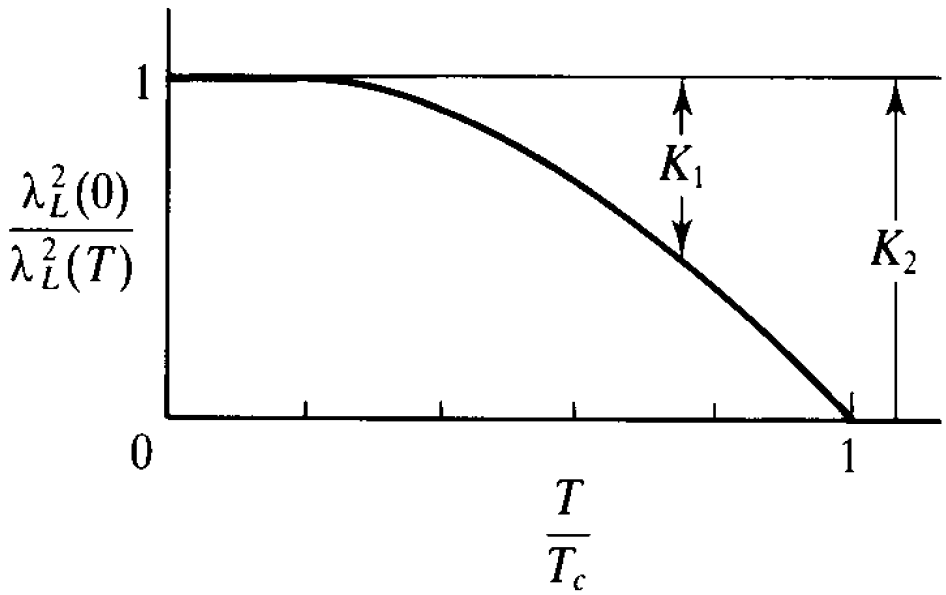
\includegraphics[width=0.5\textwidth]{immagini/Penetration_depth_BCS.png}
\end{figure}
\hspace{-0.6cm}A temperatura nulla il termine integrale si annulla e la lunghezza di penetrazione coincide con $\lambda(0)$. A temperatura finita, invece, la lunghezza di penetrazione aumenta e diverge quando ci si avvicina alla temperatura critica.\\
Possiamo inoltre valutare esplicitamente l'integrale usando la densità degli stati del superconduttore:
\begin{equation*}
   \begin{split}
      \frac{
         \lambda_L^2(0)
      }{
         \lambda_L^2(T)
      }
      &=
      1
      -
      \int_{-\infty}^{+\infty}
      \dd{\xi}
      \frac{
         N_s(E)
      }{
         N_s(0)
      }
      \qty(
         -
         \eval{\pdv{f}{E}}_{\delta=0}
      )
      \\[0.3cm]
      &=
      1
      -
      2
      \int_{\Delta}^{+\infty}
      \dd{E}
      \frac{
         E
      }{
         \sqrt{
            E^2-|\Delta|^2
         }
      }
      \qty(
         -
         \eval{\pdv{f}{E}}_{\delta=0}
      )
   \end{split}
\end{equation*}
Otteniamo così una forma esplicita della lunghezza di penetrazione in funzione della temperatura, espressa in termini della densità degli stati derivata dalle eccitazioni del superconduttore.\\
Questo mostra come sia possibile utilizzare la teoria microscopica BCS, e in particolare le eccitazioni rispetto allo stato fondamentale BCS, per derivare proprietà macroscopiche del superconduttore a temperatura finita, ottenendo una descrizione quantitativa della lunghezza di penetrazione e della risposta elettromagnetica del sistema.